\begin{bt}%[2H5V2-4]
% nguon: Archive/SP_SauLuoi_2024-2025/Sp_GHKII/data/GHKII/1-TN-DS-TLN-THPT-NgocLac-ThanhHoa-GHKII-NH24-25.tex #344
%[KNTT - Lớp 11 - Ôn tập giữa học kì 2 -THPT Ngọc Lạc - Thanh Hoá]%[TheHung Nguyễn]
	Cho tứ diện $S.ABC$ trong đó $SA \perp (ABC)$, tam giác $ABC$ vuông tại $A$ và $SA = 1$, $AB = 2$, $AC = 3$. Gọi $K$ là trực tâm của tam giác $SBC$. Tính độ dài $AK$.	
	\loigiai{\immini{	Chọn hệ tọa độ vuông góc $Oxyz$ sao cho $A$ là gốc tọa độ $A(0; 0; 0)$. Vì tam giác $ABC$ vuông tại $A$, ta có thể đặt các cạnh $AB$ và $AC$ nằm trên các trục $Ox$ và $Oy$ tương ứng. Vì $SA \perp (ABC)$, cạnh $SA$ nằm trên trục $Oz$.\\
			Khi đó 	$A(0; 0; 0)$,  $B(2; 0; 0)$, $C(0; 3; 0)$, $S(0; 0; 1)$, $\vec{BC}(-2; 3; 0)$, $\vec{SC}(0; 3; -1)$.
		}{\begin{tikzpicture}[scale=.75, font=\footnotesize, line join=round, line cap=round, >=stealth]
				\def\h{3}
				\path
				(0,0) coordinate (A)
				(0:4) coordinate (B)
				--++(-160:3) coordinate (C)
				(90:3)coordinate (S);			
				\coordinate (H) at ($(C)!1/3!(B)$);
				\coordinate (L) at ($(C)!1/3!(S)$);
				\coordinate (x) at ($(A)!1.45!(C)$);
				\coordinate (y) at ($(A)!1.45!(B)$);
				\coordinate (z) at ($(A)!1.45!(S)$);
				\path(intersection of S--H and B--L) coordinate (K);
				 	\draw [->] (B)--(y) node[below]{$y$} ;
				 	\draw [->] (C)--(x) node[below]{$x$} ;
					\draw [->] (S)--(z) node[left]{$z$} ;
				\draw (C)--(A)--(S)--(B) (S)--(C)--(B) (S)--(H) (B)--(L) ;
				\draw[dashed] (A)--(B);			
				\foreach \x/\g in {B/-90,S/45,A/180,C/200,H/-90,L/180,K/45}  \fill (\x) circle (1pt)+(\g:.35)node {$\x$};	
				\draw pic[angle radius=3mm,draw=blue,fill=green!50,opacity=.5,angle eccentricity=2] {right angle = S--A--C};
				\draw pic[angle radius=3mm,draw=blue,fill=green!50,opacity=.5,angle eccentricity=2] {right angle = S--H--B};			
		\end{tikzpicture}}
		Phương trình đường thẳng $BC\colon\heva{&x=2-2t\\&y=3t\\&z=0}$ và $SC\colon\heva{&x=0\\&y=3u\\&z=1-u.}$\\
		Gọi $H(2-2t;3t;0)$ là chân đường cao kẻ từ $S$ tới $BC$. Suy ra $\vec{SH} = (2 - 2t; 3t; -1)$.\\
		Ta có 
		$\vec{SH} \cdot \vec{BC} = 0\Leftrightarrow
		(2 - 2t)(-2) + (3t)(3) + (-1)(0) = 0 \Rightarrow t = \dfrac{4}{13}$.
		Do đó $H\left(\dfrac{18}{13}; \dfrac{12}{13}; 0\right)$.
		Tương tự $L$ là chân đường cao kẻ từ $B$ tới $SC$. Suy ra $L\left(0, \dfrac{3}{10}, \dfrac{9}{10}\right)$.\\
		Ta có $\vec{SH}=\left(\dfrac{18}{13};\dfrac{12}{13}; -1\right)$ và $\vec{BL}=\left(-2;\dfrac{3}{10};\dfrac{9}{10}\right) $.\\
		Phương trình đường thẳng $SH\colon\heva{&x=\dfrac{18}{13}t\\&y=\dfrac{12}{13}t\\&z=1-t}$ và $BL\colon \heva{&x=2-2u\\&y=\dfrac{3}{10}u\\&z=\dfrac{9}{10}u.}$\\
		Gọi $K$ là trực tâm $\triangle SBC$ nên $K$ là giao điểm của $SH$ và $BL$.\\
		Khi đó tọa độ điểm $K$ là nghiệm của hệ phương trình $\heva{&x=\dfrac{18}{13}t\\&y=\dfrac{12}{13}t\\&z=1-t\\&x=2-2u\\&y=\dfrac{3}{10}u\\&z=\dfrac{9}{10}u}\Leftrightarrow \heva{&t=\dfrac{13}{49}\\&u=\dfrac{40}{49}}.$\\
		Vậy tọa độ điểm $K\left(\dfrac{18}{49};\dfrac{12}{49};\dfrac{36}{49}.\right)$\\
		Suy ra $\vec{AK}=\left(\dfrac{18}{49};\dfrac{12}{49};\dfrac{36}{49}\right)\Rightarrow AK=\sqrt{\left(\dfrac{18}{49}\right)^2 + \left(\dfrac{12}{49}\right)^2 + \left(\dfrac{36}{49}\right)^2}=\dfrac{6}{7}$.\\
		Vậy độ dài $AK = \dfrac{6}{7}$.
	}
	
\end{bt}

\begin{bt}%[2H5V1-7]
% nguon: Archive/2024/0. [LVH] BG - 12 New - 4in1-20240625T224301Z-001/0. [LVH] BG - 12 New - 4in1/data/data_C5/Bai1-Dang8-Bai-toan-thuc-te-cuc-tri.tex #1201
%[Bài giảng 12 New - 4in1, Đoàn Hùng]
	[KNTT]
	Một vật thể chuyển động trong không gian $Oxyz$. Tại mỗi thời điểm $t$, vật thể ở vị trí $M(\cos t-\sin t;\cos t+\sin t;\cos t)$.
	\begin{enumerate}
		\item Xác định tọa độ của vị trí $M_1$, $M_2$, $M_3$ của vật tương ứng với các thời điểm $t=0$, $t=\dfrac{\pi}{2}$, $t=\pi$.
		\item Chứng minh rằng $M_1$, $M_2$, $M_3$ không thẳng hàng và viết phương trình mặt phẳng $(M_1M_2M_3)$.
		\item Vị trí $M(\cos t-\sin t;\cos t+\sin t;\cos t)$ có luôn thuộc mặt phẳng $(M_1M_2M_3)$ hay không?
	\end{enumerate}
	\loigiai{
		\begin{enumerate}
			\item Tại thời điểm $t=0$, ta có $M_1=(\cos 0-\sin 0;\cos 0+\sin 0;\cos 0)=(1;1;1)$.\\
			Tại thời điểm $t=\dfrac{\pi}{2}$, ta có $M_2=\left(\cos \dfrac{\pi}{2}-\sin \dfrac{\pi}{2};\cos \dfrac{\pi}{2}+\sin \dfrac{\pi}{2};\cos \dfrac{\pi}{2}\right)=(-1;1;0)$.\\
			Tại thời điểm $t=\pi$, ta có $M_3=(\cos \pi-\sin \pi;\cos \pi+\sin \pi;\cos \pi)=(-1;-1;-1)$.
			\item Hai véc-tơ $\vec{M_1M_2}=(-2;0;-1)$, $\vec{M_1M_3}=(-2;-2;-2)$ không cùng phương nên ba điểm $M_1$, $M_2$, $M_3$ không thẳng hàng.\\
			Mặt phẳng $(M_1M_2M_3)$ có cặp véc-tơ chỉ phương $\vec{M_1M_2}=(-2;0;-1)$, $\vec{M_1M_3}=(-2;-2;-2)$ nên có véc-tơ pháp tuyến $\vec n=[\vec{M_1M_2},\vec{M_1M_3}]=(-2;-2;4)$.\\
			Mặt phẳng $(M_1M_2M_3)$ đi qua $M_1(1;1;1)$ và có véc-tơ pháp tuyến $\vec n=(-2;-2;4)$ nên có phương trình
			$$-2(x-1)-2(y-1)+4(z-1)=0\Leftrightarrow x+y-2z=0.$$
			\item Ta có $(\cos t-\sin t)+(\cos t+\sin t)-2\cos t=0$ nên điểm $M(\cos t-\sin t;\cos t+\sin t;\cos t)$ luôn thuộc mặt phẳng $(M_1M_2M_3)$.
		\end{enumerate}
	}	
\end{bt}

\begin{bt}%[2H5V1-7]
% nguon: Archive/2024/0. [LVH] BG - 12 New - 4in1-20240625T224301Z-001/0. [LVH] BG - 12 New - 4in1/data/data_C5/Bai1-Dang8-Bai-toan-thuc-te-cuc-tri.tex #1204
%[Bài giảng 12 New - 4in1, Đoàn Hùng]
	[KNTT]
	Trong một kì thi tuyển sinh có ba môn thi Toán, Văn, Tiếng Anh. Trong không gian $Oxyz$, người ta biểu diễn kết quả thi của mỗi thí sinh bởi điểm có hoành độ, tung độ, cao độ tương ứng là điểm Toán, Văn, Tiếng Anh của thí sinh đó.
	\begin{enumerate}[a)]
		\item  Chứng minh rằng các điểm biểu diễn tương ứng với các thi sinh có tổng số điểm ba môn thi bằng $27$ (nếu có) cùng thuộc mặt phẳng có phương trình $x+y+z-27=0$.
		\item  Chứng minh rằng tồn tại một số mặt phẳng đôi một song song với nhau sao cho hai điểm biểu diễn ứng với hai thí sinh có tổng số điểm thi bằng nhau thì cùng thuộc một mặt phẳng trong số các mặt phẳng đó.		 
	\end{enumerate}
	\loigiai
	{
		Gọi $x,y,z$ lần lượt là điểm thi ba môn Toán, Văn, Tiếng Anh. 
		\begin{enumerate}[a)]
			\item Các thí sinh có tổng số điểm ba môn bằng $27$ tức là $x+y+z=27 \Leftrightarrow x+y+z-27=0$. Do đó các điểm biểu diễn này cùng thuộc mặt phẳng có phương trình $x+y+z-27=0$.
			\item Nếu tổng điểm ba môn của một thí sinh là $m$ thì điểm biểu diễn số điểm của thí sinh đó thuộc mặt phẳng $(P_m)\colon x+y+z-m=0$. Nếu tổng điểm ba môn của một thí sinh là $n$ thì điểm biểu diễn số điểm của thí sinh đó thuộc mặt phẳng $(P_n)\colon x+y+z-n=0$.\\
			Nếu $m\ne n$ thì ta có $(P_m)\parallel (P_n)$.
		\end{enumerate}
	}
\end{bt}

\begin{bt}%[2H5H1-7]
% nguon: Archive/2024/0. [LVH] BG - 12 New - 4in1-20240625T224301Z-001/0. [LVH] BG - 12 New - 4in1/data/data_C5/Bai1-Dang8-Bai-toan-thuc-te-cuc-tri.tex #1205
%[Bài giảng 12 New - 4in1, Đoàn Hùng]
	[KNTT]
	Trong không gian $Oxyz$, một ngôi nhà có sàn nhà thuộc mặt phẳng $Oxy$, trần nhà tầng $1$ thuộc mặt phẳng $z-1=0$, mái nhà tầng $2$ thuộc mặt phẳng $x+y+50z-100=0$. Hỏi trong ba mặt phẳng tương ứng chứa sàn nhà, trẩn tầng $1$, mái tầng $2$, hai mặt phẳng nào song song với nhau?
	\loigiai{
		Mặt phẳng $Oxy$ có phương trình $z=0$. Do đó trần nhà và sàn nhà song song với nhau.
	}
\end{bt}

\begin{bt}%[2H5V1-7]
% nguon: Archive/2024/0. [LVH] BG - 12 New - 4in1-20240625T224301Z-001/0. [LVH] BG - 12 New - 4in1/data/data_C5/Bai1-Dang8-Bai-toan-thuc-te-cuc-tri.tex #1209
%[Bài giảng 12 New - 4in1, Đoàn Hùng]
	[CD]
	Hình $17$ minh hoạ hình ảnh hai mái nhà của một nhà kho trong không gian với hệ toạ độ $Oxyz$ (đơn vị trên mỗi trục toạ độ là mét). Các bức tường của nhà kho đều được xây vuông góc với mặt đất.
	\begin{center}
		\begin{tikzpicture}[line join = round, line cap = round,>=stealth,font=\footnotesize,scale=.3,declare function={gx=30;gy=140;gop=atan(6/5);op=sqrt(5^2+6^2);}]
			\path 
			(0,0) coordinate (O)
			(0,9) coordinate (D)
			(gx:5) coordinate (P1)
			($(P1)+(0,6)$) coordinate (P)
			(gx:11) coordinate (A1)
			($(A1)+(0,9)$) coordinate (A)
			(gy:14) coordinate (C1)
			($(C1)+(0,9)$) coordinate (C)
			($(C)-(D)+(P)$) coordinate (Q)
			($(Q)-(P)+(A)$) coordinate (B)
			($(B)-(0,9)$) coordinate (B1)
			(gx:13) coordinate (x)
			(gy:17) coordinate (y)
			(0,20) coordinate (z)
			;
			\draw[->,>=stealth] (O)node[below]{$O$}--(x)node[below]{$x$};
			\draw[->,>=stealth] (O)--(y)node[left]{$y$};
			\draw[->,>=stealth] (O)--(z)node[right]{$z$};
			\draw (C1)--(C)node[above]{$C(0;20;10)$}--(Q)--(B)node[above]{$B(10;20;10)$}--(A)--(P)--(D)node[below left]{$D(0;0;9)$}--(C) (A)node[right]{$A(10;0;9)$}--(A1) (Q)--(P)node[shift={(-0.2,-0.4)}]{$P\left(5;0;6\right)$};
			\draw[dashed] (C1)--(B1)--(A1) (B)--(B1);
			\foreach \x/\gm in {D/180,P/90,A/0,C/90,Q/0,B/90,O/-90} \fill (\x) circle (3pt);
		\end{tikzpicture}
	\end{center}
	\begin{enumerate}[a)]
		\item Lập phương trình của hai mặt phẳng tương ứng mỗi mái nhà.
		\item Tìm tọa độ của điểm $Q$.
		\item Tìm toạ độ của véc-tơ $\vec{PQ}$.
	\end{enumerate} 
	\loigiai{
		\begin{enumerate}[a)]
			\item Hai mặt phẳng tương ứng mỗi mái nhà là $(ABP)$ và $(CDP)$.
			\begin{itemize}
				\item Do mặt phẳng $(ABP)$ có cặp véc-tơ chỉ phương là $\vec{AB}=(0;20;1)$, $\vec{AP}=(-5;0;-3)$ nên có một véc-tơ pháp tuyến là
				\[\left[\overrightarrow{AB},\overrightarrow{AP}\right]=\left(\begin{vmatrix}
					20 & 1\\
					0 & -3
				\end{vmatrix};
				\begin{vmatrix}
					1 & 0\\
					-3 & -5
				\end{vmatrix};
				\begin{vmatrix}
					0 & 20\\
					-5 & 0
				\end{vmatrix}
				\right)=\left(-60;-5;100\right)\]	
				Mà mặt phẳng $(ABP)$ đi qua điểm $A(10;0;9)$ nên có phương trình là
				$$-60(x-10)-5(y-0)+100(z-9)=0 \Leftrightarrow 12x+y-20z+60=0.$$
				\item Do mặt phẳng $(CDP)$ có cặp véc-tơ chỉ phương là $\vec{DP}=(5;0;-3)$, $\vec{DC}=(0;20;1)$ nên có một véc-tơ pháp tuyến là
				$$[\vec{DP},\vec{DC}]=\left(\left|\begin{array}{cc}
					0 & -3\\
					20 & 1
				\end{array}\right|;\left|\begin{array}{cc}
					-3 & 5\\
					1 & 0
				\end{array}\right|;\left|\begin{array}{cc}
					5 & 0\\
					0 & 20
				\end{array}\right|\right)=(60;-5;100).$$
				Mà mặt phẳng $(CDP)$ đi qua điểm $D(0;0;9)$ nên có phương trình là
				$$60(x-0)-5(y-0)+100(z-9)=0 \Leftrightarrow 12x-y+20z-180=0.$$
			\end{itemize}
			\item Vì các bức tường của nhà kho đều được xây vuông góc với mặt đất nên với hệ tọa độ trên ta có $Q(x;20;z)$.\\
			Do điểm $Q$ thuộc mặt phẳng $(ABP)$ nên tọa độ của điểm $Q$ thoả mãn $12x+20-20z+60=0$ tức là $3x-5z=-20$.\\
			Do điểm $Q$ thuộc mặt phẳng $(CDP)$ nên tọạ độ của điểm $Q$ thoả mãn $12x-20+20z-180=0$, tức là $3x+5z=50$.\\
			Ta có hệ phương trình $\heva{&3x-5z=-20\\&3x+5z=50} \Leftrightarrow \heva{&x=5\\&z=7.}$\\
			Vậy $Q(5;20;7)$.
			\item Với $P(5;0;6)$ và $Q(5;20;7)$ ta có $\vec{PQ}=(0;20;1)$.
		\end{enumerate}
	}
\end{bt}

\begin{bt}%[2H5N2-2]
% nguon: Archive/2024/0. [LVH] BG - 12 New - 4in1-20240625T224301Z-001/0. [LVH] BG - 12 New - 4in1/data/data_C5/Bai2-Dang5.tex #1221
[CTST,Mức độ 1]%[BG12, Hữu Bình]
	Cho đường thẳng $d$ có phương trình tham số $\left\{ \begin{array}{l}
		x=-2+6t\\
		y=11+2t\\
		z=4t
	\end{array}\right. \left( t \in \mathbb{R}\right)$.
	\begin{enumerate}
		\item Tìm hai vectơ chỉ phương của $d$.
		\item Tìm các điểm trên $d$ ứng với $t$ lần lượt bằng $0;2;-3$.
	\end{enumerate}
	\loigiai{
		\begin{enumerate}
			\item Từ phương trình tham số, ta có $\overrightarrow{a}=\left( 6;2;4 \right)$ là một vectơ chỉ phương của $d$.\\
			Chọn $\overrightarrow{b}=\dfrac{1}{2}\overrightarrow{a}=\left( 3;1;2 \right)$, ta có $\overrightarrow{b}$ cũng là một vectơ chỉ phương của $d$.
			\item Thay $t=0$ vào phương trình tham số của $d$, ta được:\\
			\begin{center}
				$\left\{ \begin{array}{l}
					x=-2+6 \cdot 0\\
					y= 11+2 \cdot 0\\
					z=4 \cdot 0
				\end{array}\right.$ hay $\left\{ \begin{array}{l}
					x=-2\\
					y= 11\\
					z=0.
				\end{array}\right.$
			\end{center}
			Vậy $A\left( -2;11;0 \right)$.\\
			Tương tự, với $t=2$ thì $B\left( 10;15;8 \right)$, với $t=-3$ thì $C\left( -20;5;-12 \right)$.
		\end{enumerate}
	}
\end{bt}

\begin{bt}%[2H5N2-3]
% nguon: Archive/2024/0. [LVH] BG - 12 New - 4in1-20240625T224301Z-001/0. [LVH] BG - 12 New - 4in1/data/data_C5/Bai2-Dang5.tex #1222
[CKP, Mức độ 1]%[BG12, Hữu Bình]
	Trong không gian $Oxyz$, cho đường thẳng $d$ đi qua điểm $M(2;-2;1)$ và có vectơ chỉ phương
	là $\overrightarrow{a} = (1;-1; 2)$.
	\begin{listEX}
		\item  Viết phương trình tham số của đường thẳng $d$.
		\item  Trong hai điểm $A (3; -3; 3)$ và $B (1;-1; 1)$ điểm nào thuộc $d$?
	\end{listEX}
	\loigiai{
		\begin{listEX}
			\item  Phương trình tham số của $d$ là $\heva{&x=2+t\\&y=-2-t\\&z=1+2t} (t\in \mathbb{R}).$
			\item Điểm $M_\circ(x_\circ ; y_\circ ; z_\circ)$ thuộc đường thẳng $d$ khi và chỉ khi có giá trị $t$ thoả mãn hệ
			phương trình $\heva{&x_\circ = 2 + t\\&y_\circ = -2 - t\\&z_\circ=1+2t.}$\\
			Ta có:
			\begin{itemize}
				\item Với $A(3; -3; 3)$, ta xét $\heva{&3 = 2 + t\\&-3 = -2 - t\\&3=1+2t.}$\\
				Hệ phương trình này có nghiệm duy nhất $t = 1$ nên $A$ thuộc $d$ ứng với $t = 1$.
				\item Với $B(1;-1; 1)$, ta xét $\heva{&1 = 2 + t\\&-1 = -2 - t\\&1=1+2t.}$\\
				Hệ phương trình này vô nghiệm nên $B$ không thuộc $d$.
			\end{itemize}
		\end{listEX}
	}
\end{bt}

\begin{bt}%[2H5N2-2]
% nguon: Archive/2024/0. [LVH] BG - 12 New - 4in1-20240625T224301Z-001/0. [LVH] BG - 12 New - 4in1/data/data_C5/Bai2-Dang5.tex #1223
[CKP, Mức độ 1]%[BG12, Hữu Bình]
	Trong không gian $Oxyz$, cho đường thẳng $d$ có phương trình chính tắc \[\dfrac{x - 3}{2} = \dfrac{y + 2}{3} =\dfrac{z}{6}.\]
	\begin{listEX}
		\item  Tìm toạ độ một vectơ chỉ phương  của $d$.
		\item  Trong hai điểm $A (1; -5; -6)$ và $B (3; -2; 1)$, điểm nào thuộc $d$?
	\end{listEX}
	\loigiai{
		\begin{listEX}
			\item  Một vectơ chỉ phương  của $d$ là $\overrightarrow{a} = (2; 3; 6).$
			\item  Một điểm thuộc $d$ khi toạ độ của điểm đó thoả mãn phương trình chính tắc của $d$:
			\[\dfrac{x - 3}{2}=\dfrac{y + 2}{3}=\dfrac{z}{6}\quad (\ast)\]
			Thay toạ độ của các điểm $A, B$ vào phương trình chính tắc $(\ast)$. Ta có:
			\begin{itemize}
				\item Điểm $A (1; -5; -6)$ thoả mãn $(\ast)$ vì $\dfrac{1-3}{2}=\dfrac{-5+2}{3}=\dfrac{-6}{6}$  nên $A$ thuộc $d$.
				\item Điểm $B (3; -2; 1)$ không thoả mãn $(\ast)$ vì $\dfrac{3-3}{2}=\dfrac{-2+2}{3} \ne \dfrac{1}{6}$ nên $B$ không thuộc $d$.
			\end{itemize}
		\end{listEX}
	}
\end{bt}

\begin{bt}%[2H5N2-3]
% nguon: Archive/2024/0. [LVH] BG - 12 New - 4in1-20240625T224301Z-001/0. [LVH] BG - 12 New - 4in1/data/data_C5/Bai2-Dang5.tex #1224
[CTST, Mức độ 1]%[BG12, Hữu Bình]
	Viết phương trình tham số của đường thẳng $d$ đi qua điểm $M_0\left( 1;2;3 \right)$ và nhận $\overrightarrow{a}=\left( 4;5;-7 \right)$ làm vectơ chỉ phương. Đường thẳng $d$ có đi qua điểm $A\left( 1;1;5 \right)$ không?
	\loigiai{
		Ta có phương trình tham số của $d$ là:
		$$\left\{ \begin{array}{l}
			x=1+4t\\
			y=2+5t\\
			z=3-7t.
		\end{array}\right.$$
		Thay $x=1$ vào phương trình $x=1+4t$, ta được $1=1+4t$, suy ra $t=0$.\\
		Thay $y=1$ và $t=0$ vào phương trình $y=2+5t$, ta thấy phương trình không 	thoả mãn. Suy ra đường thẳng $d$ không đi qua điểm $A$.
	}
\end{bt}

\begin{bt}%[2H5H2-7]
% nguon: Archive/2024/0. [LVH] BG - 12 New - 4in1-20240625T224301Z-001/0. [LVH] BG - 12 New - 4in1/data/data_C5/Bai2-Dang4.tex #1225

	Tính góc giữa hai đường thẳng $d$ và $d'$ trong mỗi trường hợp sau
	\begin{enumerate}
		\item $d\colon\dfrac{x-1}{1}=\dfrac{y+2}{2}=\dfrac{z-1}{1}$ và $d'\colon\dfrac{x-1}{1}=\dfrac{y+2}{1}=\dfrac{z-1}{2}$;
		\item $d\colon\dfrac{x+2}{1}=\dfrac{y+4}{2}=\dfrac{z+1}{2}$ và $d'\colon\heva{& x=2-2t\\&y=2-2t\\&z=1+t; }$
		\item $d\colon\heva{& x=1+t\\&y=-1+2t\\&z=-2-t }$ và $d'\colon\heva{& x=2+2t'\\&y=3+4t'\\&z=10t'. }$
	\end{enumerate}
	\loigiai
	{
		\begin{enumerate}
			\item $d$ và $d'$ có vectơ chỉ phương lần lượt là $\overrightarrow{a}=(1;2;1)$ và $\overrightarrow{a}'=(1;1;2)$.\\
			Ta có $\cos (d,d')=\dfrac{\left |1\cdot 1+2\cdot 1+1\cdot 2 \right |}{\sqrt{1^2+2^2+1^2}\cdot\sqrt{1^2+1^2+2^2}}=\dfrac{5}{6}$.\\
			Suy ra $(d,d')\approx 33^{\circ}33'$.
			\item $d$ và $d'$ có vectơ chỉ phương lần lượt là $\overrightarrow{a}=(1;2;2)$ và $\overrightarrow{a}'=(-2;-2;1)$.\\
			Ta có $\cos (d,d')=\dfrac{\left |1\cdot (-2)+2\cdot (-2)+2\cdot 1 \right |}{\sqrt{1^2+2^2+2^2}\cdot\sqrt{(-2)^2+(-2)^2+1^2}}=\dfrac{4}{9}$.\\
			Suy ra $(d,d')\approx 63^{\circ}36'$.
			\item $d$ và $d'$ có vectơ chỉ phương lần lượt là $\overrightarrow{a}=(1;2;-1)$ và $\overrightarrow{a}'=(2;4;10)$.\\
			Ta có $\cos (d,d')=\dfrac{\left |1\cdot 2+2\cdot 4+(-1)\cdot 10 \right |}{\sqrt{1^2+2^2+(-1)^2}\cdot\sqrt{2^2+4^2+10^2}}=0$.\\
			Suy ra $(d,d')=90^{\circ}$.
		\end{enumerate}
	}
\end{bt}

\begin{bt}%[2H5H2-7]
% nguon: Archive/2024/0. [LVH] BG - 12 New - 4in1-20240625T224301Z-001/0. [LVH] BG - 12 New - 4in1/data/data_C5/Bai2-Dang4.tex #1226

	Tính góc giữa đường thẳng $d$ và mặt phẳng $(P)$ trong mỗi trường hợp sau
	\begin{enumerate}
		\item $d\colon\dfrac{x+2}{2}=\dfrac{y+4}{2}=\dfrac{z+1}{1}$ và $(P)\colon x+z+24=0$;
		\item $d\colon\heva{& x=1+t\\&y=-1+2t\\&z=-2-t }$ và $(P)\colon 2x+4y-2z+23=0$.
	\end{enumerate}
	\loigiai
	{
		\begin{enumerate}
			\item Đường thẳng $d$ có vectơ chỉ phương $\overrightarrow{a}=(2;2;1)$. Mặt phẳng $(P)$ có vectơ pháp tuyến $\overrightarrow{n}=(1;0;1)$.\\
			Ta có $\sin (d,(P))=\dfrac{\left |2\cdot 1+2\cdot 0+1\cdot 1 \right |}{\sqrt{2^2+2^2+1^2}\cdot\sqrt{1^2+0^2+1^2}}=\dfrac{1}{\sqrt{2}}$.\\
			Suy ra $(d,(P))=45^{\circ}$.
			\item Đường thẳng $d$ có vectơ chỉ phương $\overrightarrow{a}=(1;2;-1)$. Mặt phẳng $(P)$ có vectơ pháp tuyến $\overrightarrow{n}=(2;-4;-2)$.\\
			Ta có $\sin (d,(P))=\dfrac{\left |1\cdot 2+2\cdot 4+(-1)\cdot (-2) \right |}{\sqrt{1^2+2^2+(-1)^2}\cdot\sqrt{2^2+4^2+(-2)^2}}=1$.\\
			Suy ra $(d,(P))=90^{\circ}$.
		\end{enumerate}
	}
\end{bt}

\begin{bt}%[2H5H1-6]
% nguon: Archive/2024/0. [LVH] BG - 12 New - 4in1-20240625T224301Z-001/0. [LVH] BG - 12 New - 4in1/data/data_C5/Bai2-Dang4.tex #1227

	Tính góc giữa hai mặt phẳng $(P)$ và $(P')$ trong mỗi trường hợp sau
	\begin{enumerate}
		\item $(P)\colon x+y-2z+9=0$ và $(P')\colon 3x-5y+z+2024=0$;
		\item $(P)\colon x+y+24=0$ và $(P')\colon y+z+24=0$;
		\item $(P)\colon 2x+4y-z+23=0$ và $(P')\colon 3x+5y+26z+2025=0$.
	\end{enumerate}
	\loigiai
	{
		\begin{enumerate}
			\item $(P)$ và $(P')$ có vectơ pháp tuyến lần lượt là $\overrightarrow{n}=(1;1;-2)$, $\overrightarrow{n}'=(3;-5;1)$.\\
			Ta có $\cos\left ((P),(P') \right )=\dfrac{\left |1\cdot 3+1\cdot (-5)+(-2)\cdot 1 \right |}{\sqrt{1^2+1^2+(-2)^2}\cdot\sqrt{3^2+(-5)^2+1^2}}=\dfrac{4}{\sqrt{210}}$.\\
			Suy ra $((P),(P'))\approx 73^{\circ}59'$.
			\item $(P)$ và $(P')$ có vectơ pháp tuyến lần lượt là $\overrightarrow{n}=(1;1;0)$, $\overrightarrow{n}'=(0;1;1)$.\\
			Ta có $\cos\left ((P),(P') \right )=\dfrac{\left |1\cdot 0+1\cdot 1+0\cdot 1 \right |}{\sqrt{1^2+1^2+0^2}\cdot\sqrt{0^2+1^2+1^2}}=\dfrac{1}{2}$.\\
			Suy ra $((P),(P'))=60^{\circ}$.
			\item $(P)$ và $(P')$ có vectơ pháp tuyến lần lượt là $\overrightarrow{n}=(2;4;-1)$, $\overrightarrow{n}'=(3-5;26)$.\\
			Ta có $\cos\left ((P),(P') \right )=\dfrac{\left |2\cdot 3+4\cdot 5+(-1)\cdot 26 \right |}{\sqrt{2^2+4^2+(-1)^2}\cdot\sqrt{3^2+5^2+26^2}}=0$.\\
			Suy ra $((P),(P'))=90^{\circ}$.
		\end{enumerate}
	}
\end{bt}

\begin{bt}%[2H5V2-7]
% nguon: Archive/2024/0. [LVH] BG - 12 New - 4in1-20240625T224301Z-001/0. [LVH] BG - 12 New - 4in1/data/data_C5/Bai2-Dang4.tex #1228

	Cho hình chóp $S.ABCD$ có đáy $ABCD$ là hình chữ nhật và $SA\perp (ABCD)$. Cho biết $AB=2a$, $AD=3a$ và $SA=2a$. Tính góc giữa:
	\begin{enumerate}
		\item Hai đường thẳng $SC$ và $BD$;
		\item Mặt phẳng $(SBD)$ và mặt đáy;
		\item Đường thẳng $SC$ và mặt phẳng $(SBD)$.
	\end{enumerate}
	\loigiai
	{
		\immini{
			Chọn hệ tọa độ $Oxyz$ sao cho các điểm có tọa độ như sau: $A(0;0;0)$, $B(2a;0;0)$, $D(0;3a;0)$, $S(0;0;2a)$. \\Trong không gian $Oxyz$ vừa chọn, ta có $C(2a;3a;0)$, $\overrightarrow{SC}=(2a;3a;-2a)$, $\overrightarrow{BD}=(-2a;3a;0)$.
			\begin{listEX}[1]
				\item Hai đường thẳng $SC$ và $BD$ có vectơ chỉ phương lần lượt là $\overrightarrow{u}=(2;3;-2)$, $\overrightarrow{v}=(-2;3;0)$.\\
				Ta có 
				\begin{eqnarray*}
					\cos (SC,BD)=\dfrac{\left |2\cdot (-2)+3\cdot 3+(-2)\cdot 0 \right |}{\sqrt{2^2+3^2+(-2)^2}\cdot\sqrt{(-2)^2+3^2+0^2}}=\dfrac{5}{\sqrt{221}}.
				\end{eqnarray*}
			\end{listEX}
		}{
			\begin{tikzpicture}[line cap=round,line join=round,scale=.7,>=stealth,font=\footnotesize ]
				\coordinate (A) at (0,0);
				\coordinate (S) at (0,3);
				\coordinate (z) at (0,4);
				\coordinate (D) at (3,0);
				\coordinate (y) at (4,0);
				\coordinate (C) at (2,-2);
				\coordinate (B) at (-1,-2);
				\coordinate (x) at ($(A)!1.5!(B)$);
				\draw[dashed](S)--(A)--(B)--(D)--(A);
				\draw (D)--(C)--(B)--(S)--(C)(S)--(D);
				\draw[->](B)--(x);
				\draw[->](S)--(z);
				\draw[->](D)--(y);
				\foreach \x/\g in {z/90,S/180,D/90,y/0,A/-45,B/180,x/-90,C/-90}
				\fill[black](\x) circle (1pt)
				($(\x)+(\g:3mm)$) node{\x};
			\end{tikzpicture}
		}
		Suy ra $(SC,BD)\approx 70^{\circ}21'$.
		\begin{enumerate}
			\setcounter{enumi}{1}
			\item Ta có phương trình mặt phẳng $(SBD)$ theo đoạn chắn là $\dfrac{x}{2a}+\dfrac{y}{3a}+\dfrac{z}{2a}=1$ hay $3x+2y+3z-6a=0$.\\
			Mặt phẳng $(SBD)$ có vectơ pháp tuyến $\overrightarrow{n}=(3;2;3)$, mặt đáy $(ABCD)$ có vectơ pháp tuyến $\overrightarrow{k}=(0;0;1)$. Gọi $\alpha$ là góc giữa mặt phẳng $(SBD)$ và mặt đáy.\\
			Ta có $\cos\alpha =\dfrac{\left |\overrightarrow{n}\cdot\overrightarrow{k} \right |}{\left |\overrightarrow{n} \right |\cdot\left |\overrightarrow{k} \right |}=\dfrac{\left |3\cdot 0+2\cdot 0+3\cdot 1 \right |}{\sqrt{3^2+2^2+3^2}\cdot\sqrt{0^2+0^2+1^2}}=\dfrac{3}{\sqrt{22}}$.\\
			Suy ra $\left ((SBD),(ABCD) \right )\approx 50^{\circ}14'$.
			\item Gọi $\beta$ là góc giữa đường thẳng $SC$ và mặt phẳng $(SBD)$.\\
			Ta có $\sin\beta =\dfrac{\left |\overrightarrow{u}\cdot\overrightarrow{n} \right |}{\left |\overrightarrow{u} \right |\cdot\left |\overrightarrow{n} \right |}=\dfrac{\left |2\cdot 3+3\cdot 2+(-2)\cdot 3 \right |}{\sqrt{2^2+3^2+(-2)^2}\cdot\sqrt{3^2+2^2+3^2}}=\dfrac{6}{\sqrt{374}}$.\\
			Suy ra $\left (SC,(SBD) \right )\approx 18^{\circ}4'$.
		\end{enumerate}
	}
\end{bt}

\begin{bt}%[2H5H2-7]
% nguon: Archive/2024/0. [LVH] BG - 12 New - 4in1-20240625T224301Z-001/0. [LVH] BG - 12 New - 4in1/data/data_C5/Bai2-Dang4.tex #1229

	Tính góc giữa đường thẳng $d$ và mặt phẳng $(P)$ trong mỗi trường hợp sau
	\begin{listEX}[1]
		\item $d\colon\heva{& x=11+3t\\&y=-11+t\\&z=-21-2t }$ và $(P)\colon 6x+2y-4z+7=0$;
		\item $d\colon\dfrac{x-3}{2}=\dfrac{y+4}{4}=\dfrac{z-5}{2}$ và $(P)\colon 2x+2y-4z+1=0$;
		\item $d\colon \dfrac{x+3}{4}=\dfrac{y+5}{4}=\dfrac{z+11}{2}$ và $(P)\colon 2y-4z+7=0$.
	\end{listEX}
	\loigiai
	{
		\begin{listEX}[1]
			\item Đường thẳng $d$ có vectơ chỉ phương $\overrightarrow{a}=(3;1;-2)$. Mặt phẳng $(P)$ có vectơ pháp tuyến $\overrightarrow{n}=(6;2;-4)$.\\
			Ta có $\sin (d,(P))=\dfrac{\left |3\cdot 6+1\cdot 2+(-2)\cdot (-4) \right |}{\sqrt{3^2+1^2+(-2)^2}\cdot\sqrt{6^2+2^2+(-4)^2}}=1$.\\
			Suy ra $(d,(P))=90^{\circ}$.
			\item Đường thẳng $d$ có vectơ chỉ phương $\overrightarrow{a}=(2;4;2)$. Mặt phẳng $(P)$ có vectơ pháp tuyến $\overrightarrow{n}=(2;2;-4)$.\\
			Ta có $\sin (d,(P))=\dfrac{\left |2\cdot 2+4\cdot 2+2\cdot (-4) \right |}{\sqrt{2^2+4^2+2^2}\cdot\sqrt{2^2+2^2+(-4)^2}}=\dfrac{1}{6}$.\\
			Suy ra $(d,(P))\approx 9^{\circ}36'$.
			\item Đường thẳng $d$ có vectơ chỉ phương $\overrightarrow{a}=(4;4;2)$. Mặt phẳng $(P)$ có vectơ pháp tuyến $\overrightarrow{n}=(0;2;-4)$.\\
			Ta có $\sin (d,(P))=\dfrac{\left |4\cdot 0+4\cdot 2+2\cdot (-4) \right |}{\sqrt{4^2+4^2+2^2}\cdot\sqrt{0^2+2^2+(-4)^2}}=0$.\\
			Suy ra $(d,(P))=0^{\circ}$.
		\end{listEX}
	}
\end{bt}

\begin{bt}%[2H5H1-6]
% nguon: Archive/2024/0. [LVH] BG - 12 New - 4in1-20240625T224301Z-001/0. [LVH] BG - 12 New - 4in1/data/data_C5/Bai2-Dang4.tex #1230

	Tính góc giữa hai mặt phẳng $(P)$ và $(P')$ trong mỗi trường hợp sau
	\begin{listEX}[1]
		\item $(P)\colon 3x+7y-z+4=0$ và $(P')\colon x+y-10z+2025=0$.
		\item $(P)\colon x+y-2z+2024=0$ và $(P')\colon 3x-5y+z+9=0$.
		\item $(P)\colon x+z+3=0$ và $(P')\colon 3y+3z+5=0$.
	\end{listEX}
	\loigiai
	{
		\begin{listEX}[1]
			\item $(P)$ và $(P')$ có vectơ pháp tuyến lần lượt là $\overrightarrow{n}=(3;7;-1)$, $\overrightarrow{n}'=(1;1;-10)$.\\
			Ta có $\cos\left ((P),(P') \right )=\dfrac{\left |3\cdot 1+7\cdot 1+(-1)\cdot (-10) \right |}{\sqrt{3^2+7^2+(-1)^2}\cdot\sqrt{1^2+1^2+(-10)^2}}=\dfrac{10\sqrt{6018}}{3009}$.\\
			Suy ra $((P),(P'))\approx 75^{\circ}4'$.
			\item $(P)$ và $(P')$ có vectơ pháp tuyến lần lượt là $\overrightarrow{n}=(1;1;-2)$, $\overrightarrow{n}'=(3;-5;1)$.\\
			Ta có $\cos\left ((P),(P') \right )=\dfrac{\left |1\cdot 3+1\cdot (-5)+(-2)\cdot 1 \right |}{\sqrt{1^2+1^2+(-2)^2}\cdot\sqrt{3^2+(-5)^2+1^2}}=\dfrac{4}{\sqrt{210}}$.\\
			Suy ra $((P),(P'))\approx 73^{\circ}59'$.
			\item $(P)$ và $(P')$ có vectơ pháp tuyến lần lượt là $\overrightarrow{n}=(1;0;1)$, $\overrightarrow{n}'=(0;3;3)$.\\
			Ta có $\cos\left ((P),(P') \right )=\dfrac{\left |1\cdot 0+0\cdot 3+1\cdot 3 \right |}{\sqrt{1^2+1^2}\cdot\sqrt{3^2+3^2}}=\dfrac{1}{2}$.\\
			Suy ra $((P),(P')=60^{\circ}$.
		\end{listEX}
	}
\end{bt}

\begin{bt}%[2H5N1-6]
% nguon: Archive/2024/0. [LVH] BG - 12 New - 4in1-20240625T224301Z-001/0. [LVH] BG - 12 New - 4in1/data/data_C5/Bai1-Dang6-Goc-giua-hai-mp.tex #1232
[Cánh Diều, mức độ 1]%[Hoàng Thanh Phương, dự án BG12]
	Tính góc giữa hai mặt phẳng $(P_1)\colon x+y+2z-1=0$ và $(P_2)\colon 2x-y+z-2=0$.
	\loigiai{
		$(P_1)$, $(P_2)$ lần lượt có véc-tơ pháp tuyến $\overrightarrow{n}_1=(1;1;2)$ và $\overrightarrow{n}_2=(2;-1;1)$.\\
		Ta có $\cos\left((P_1),(P_2)\right)=\dfrac{\left|\overrightarrow{n}_1\cdot\overrightarrow{n}_2\right|}{\left|\overrightarrow{n}_1\right|\cdot\left|\overrightarrow{n}_2\right|}=\dfrac{|1\cdot2+1\cdot(-1)+2\cdot1|}{\sqrt{1^2+1^2+2^2}\cdot\sqrt{2^2+(-1)^2+1^2}}=\dfrac{1}{2}$.\\
		Vậy $\left((P_1),(P_2)\right)=60^\circ$.
	}
\end{bt}

\begin{bt}%[2H5N1-6]
% nguon: Archive/2024/0. [LVH] BG - 12 New - 4in1-20240625T224301Z-001/0. [LVH] BG - 12 New - 4in1/data/data_C5/Bai1-Dang6-Goc-giua-hai-mp.tex #1233
[CKP, mức độ 1]%[Hoàng Thanh Phương, dự án BG12]
	Trong không gian $Oxyz$, tính góc giữa hai mặt phẳng $(\alpha)\colon \sqrt{3}x-y+2=0$ và các mặt phẳng tọa độ $(Oxy),(Oxz),(Oyz)$
	\loigiai{
		Mặt phẳng $(\alpha),(Oxy),(Oxz),(Oyz)$ lần lượt có véc-tơ pháp tuyến là $\overrightarrow{n}=\left(\sqrt{3};-1;0\right),\overrightarrow{n_1}=\left(0;0;1\right),\overrightarrow{n_2}=\left(0;1;0\right),\overrightarrow{n_3}=\left(1;0;0\right)$.\\
		Ta có
		\begin{eqnarray*}
			\cos((\alpha),(Oxy))&=&\dfrac{|\sqrt{3}\cdot 0+(-1)\cdot 0+0\cdot 1|}{\sqrt{(\sqrt{3})^2+(-1)^2}\cdot \sqrt{0^2+0^2+1^2}}=0.\\
			\cos((\alpha),(Oxz))&=&\dfrac{|\sqrt{3}\cdot 0+(-1)\cdot 1+0\cdot 0|}{\sqrt{(\sqrt{3})^2+(-1)^2}\cdot \sqrt{0^2+1^2+0^2}}=\dfrac{1}{2}.\\
			\cos((\alpha),(Oyz))&=&\dfrac{|\sqrt{3}\cdot 1+(-1)\cdot 0+0\cdot 0|}{\sqrt{(\sqrt{3})^2+(-1)^2}\cdot \sqrt{1^2+0^2+0^2}}=\dfrac{\sqrt{3}}{2}.
		\end{eqnarray*}
		Vậy $((\alpha),(Oxy))=90^{\circ},((\alpha),(Oxz))=60^{\circ},((\alpha),(Oyz))=30^{\circ}$.
	}
\end{bt}

\begin{bt}%[2H5N1-6]
% nguon: Archive/2024/0. [LVH] BG - 12 New - 4in1-20240625T224301Z-001/0. [LVH] BG - 12 New - 4in1/data/data_C5/Bai1-Dang6-Goc-giua-hai-mp.tex #1234
[KNTT, mức độ 1]%[Hoàng Thanh Phương, dự án BG12]
	Trong không gian $Oxyz$, tính góc giữa hai mặt phẳng $(P)\colon x+2y+2z-1=0$ và $(Q)\colon x+y-z+1=0$.
	\loigiai{\hfill
		
		\noindent Các mặt phẳng $(P)$, $(Q)$ tương ứng có các véc-tơ pháp tuyến là $\overrightarrow{n}=(1; 2; 2)$, $\overrightarrow{n'}=(1; 1;-1)$.\\
		Ta có $\cos ((P),(Q))=\dfrac{|1\cdot 1+2\cdot 1+2\cdot(-1)|}{\sqrt{1^2+2^2+2^2} \cdot \sqrt{1^2+1^2+(-1)^2}}=\dfrac{\sqrt{3}}{9}$.\\
		Do đó $((P),(Q)) \approx 78{,}9^{\circ}$.}
\end{bt}

\begin{bt}%[2H5N1-6]
% nguon: Archive/2024/0. [LVH] BG - 12 New - 4in1-20240625T224301Z-001/0. [LVH] BG - 12 New - 4in1/data/data_C5/Bai1-Dang6-Goc-giua-hai-mp.tex #1235
[CTST, mức độ 1]%[Hoàng Thanh Phương, dự án BG12]
	Tính góc giữa hai mặt phẳng $(P)$ và $(P')$ trong mỗi trường hợp sau
	\begin{enumerate}
		\item $(P)\colon x+y-2z+9=0$ và $(P')\colon 3x-5y+z+2024=0$;
		\item $(P)\colon x+y+24=0$ và $(P')\colon y+z+24=0$;
		\item $(P)\colon 2x+4y-z+23=0$ và $(P')\colon 3x+5y+26z+2025=0$.
	\end{enumerate}
	\loigiai
	{
		\begin{enumerate}
			\item $(P)$ và $(P')$ có véc-tơ pháp tuyến lần lượt là $\overrightarrow{n}=(1;1;-2)$, $\overrightarrow{n}'=(3;-5;1)$.\\
			Ta có $\cos\left ((P),(P') \right )=\dfrac{\left |1\cdot 3+1\cdot (-5)+(-2)\cdot 1 \right |}{\sqrt{1^2+1^2+(-2)^2}\cdot\sqrt{3^2+(-5)^2+1^2}}=\dfrac{4}{\sqrt{210}}$.\\
			Suy ra $((P),(P'))\approx 73^{\circ}59'$.
			\item $(P)$ và $(P')$ có véc-tơ pháp tuyến lần lượt là $\overrightarrow{n}=(1;1;0)$, $\overrightarrow{n}'=(0;1;1)$.\\
			Ta có $\cos\left ((P),(P') \right )=\dfrac{\left |1\cdot 0+1\cdot 1+0\cdot 1 \right |}{\sqrt{1^2+1^2+0^2}\cdot\sqrt{0^2+1^2+1^2}}=\dfrac{1}{2}$.\\
			Suy ra $((P),(P'))=60^{\circ}$.
			\item $(P)$ và $(P')$ có véc-tơ pháp tuyến lần lượt là $\overrightarrow{n}=(2;4;-1)$, $\overrightarrow{n}'=(3-5;26)$.\\
			Ta có $\cos\left ((P),(P') \right )=\dfrac{\left |2\cdot 3+4\cdot 5+(-1)\cdot 26 \right |}{\sqrt{2^2+4^2+(-1)^2}\cdot\sqrt{3^2+5^2+26^2}}=0$.\\
			Suy ra $((P),(P'))=90^{\circ}$.
		\end{enumerate}
	}
\end{bt}

\begin{bt}%[2H5N1-6]
% nguon: Archive/2024/0. [LVH] BG - 12 New - 4in1-20240625T224301Z-001/0. [LVH] BG - 12 New - 4in1/data/data_C5/Bai1-Dang6-Goc-giua-hai-mp.tex #1236
%[Hoàng Thanh Phương, dự án BG12]
	Tính góc giữa hai mặt phẳng $(P)$ và $(P')$ trong mỗi trường hợp sau
	\begin{enumerate}
		\item $(P)\colon 3x+7y-z+4=0$ và $(P')\colon x+y-10z+2025=0$.
		\item $(P)\colon x+y-2z+2024=0$ và $(P')\colon 3x-5y+z+9=0$.
		\item $(P)\colon x+z+3=0$ và $(P')\colon 3y+3z+5=0$.
	\end{enumerate}
	\loigiai
	{
		\begin{enumerate}
			\item $(P)$ và $(P')$ có véc-tơ pháp tuyến lần lượt là $\overrightarrow{n}=(3;7;-1)$, $\overrightarrow{n}'=(1;1;-10)$.\\
			Ta có $\cos\left ((P),(P') \right )=\dfrac{\left |3\cdot 1+7\cdot 1+(-1)\cdot (-10) \right |}{\sqrt{3^2+7^2+(-1)^2}\cdot\sqrt{1^2+1^2+(-10)^2}}=\dfrac{10\sqrt{6018}}{3009}$.\\
			Suy ra $((P),(P'))\approx 75^{\circ}4'$.
			\item $(P)$ và $(P')$ có véc-tơ pháp tuyến lần lượt là $\overrightarrow{n}=(1;1;-2)$, $\overrightarrow{n}'=(3;-5;1)$.\\
			Ta có $\cos\left ((P),(P') \right )=\dfrac{\left |1\cdot 3+1\cdot (-5)+(-2)\cdot 1 \right |}{\sqrt{1^2+1^2+(-2)^2}\cdot\sqrt{3^2+(-5)^2+1^2}}=\dfrac{4}{\sqrt{210}}$.\\
			Suy ra $((P),(P'))\approx 73^{\circ}59'$.
			\item $(P)$ và $(P')$ có véc-tơ pháp tuyến lần lượt là $\overrightarrow{n}=(1;0;1)$, $\overrightarrow{n}'=(0;3;3)$.\\
			Ta có $\cos\left ((P),(P') \right )=\dfrac{\left |1\cdot 0+0\cdot 3+1\cdot 3 \right |}{\sqrt{1^2+1^2}\cdot\sqrt{3^2+3^2}}=\dfrac{1}{2}$.\\
			Suy ra $((P),(P')=60^{\circ}$.
		\end{enumerate}
	}
\end{bt}

\begin{bt}%[2H5N1-6]
% nguon: Archive/2024/0. [LVH] BG - 12 New - 4in1-20240625T224301Z-001/0. [LVH] BG - 12 New - 4in1/data/data_C5/Bai1-Dang6-Goc-giua-hai-mp.tex #1237
[Mức độ 1]%[Hoàng Thanh Phương, dự án BG12]
	Tính góc giữa hai mặt phẳng $(P)\colon 4y+4z+1=0$ và $(P')\colon 7x+7z+2=0$.
	\loigiai
	{
		$(P)$ và $(P')$ có véc-tơ pháp tuyến lần lượt là $\overrightarrow{n}=(0;4;4)$ và $\overrightarrow{n}'=(7;0;7)$.\\
		Ta có $\cos \left ((P),(P') \right )=\dfrac{\left |0\cdot 7+4\cdot 0+4\cdot 7 \right |}{\sqrt{0^2+4^2+4^2}\cdot\sqrt{7^2+0^2+7^2}}=\dfrac{1}{2}$.\\
		Suy ra $\left ((P),(P') \right )=60^{\circ}$.
	}
\end{bt}

\begin{bt}%[2H5N1-6]
% nguon: Archive/2024/0. [LVH] BG - 12 New - 4in1-20240625T224301Z-001/0. [LVH] BG - 12 New - 4in1/data/data_C5/Bai1-Dang6-Goc-giua-hai-mp.tex #1238
[Mức độ 1]%[Hoàng Thanh Phương, dự án BG12]
	Trong không gian với hệ tọa độ $Oxyz$, tìm tập hợp tất cả các giá trị thực của tham số $m$ để góc giữa hai mặt phẳng $(P)\colon x+2y+z+2=0$ và $(Q)\colon -x+(2m^2-1)y+2z-1=0$ bằng $60^\circ$.
	\loigiai{
Ta có $\vec{n}_{(P)}=(1;2;1)$, $\vec{n}_{(Q)}=(-1;2m^2-1;2)$. 
Ta có 
\begin{eqnarray*}
	&&\cos \left((P),(Q)\right)=60^\circ \\
	&\Leftrightarrow &\dfrac{|-1+4m^2-2+2|}{\sqrt{6}\cdot \sqrt{4m^4-4m^2+6}}=\dfrac{1}{2} \\
	&\Leftrightarrow &4(4m^2-1)^2=6(4m^4-4m^2+6) \\
	&\Leftrightarrow &40m^4-8m^2-32=0 \\
	&\Leftrightarrow &\hoac{&m^2=1\\&m^2=-\dfrac{4}{5}~(\text{loại})}\Leftrightarrow m=\pm 1.
\end{eqnarray*}
Vậy với $m=1$ hoặc $m=-1$ thì góc giữa hai mặt phẳng $(P)$ và $(Q)$ bằng $60^\circ$.
}
\end{bt}

\begin{bt}%[2H5H1-6]
% nguon: Archive/2024/0. [LVH] BG - 12 New - 4in1-20240625T224301Z-001/0. [LVH] BG - 12 New - 4in1/data/data_C5/Bai1-Dang6-Goc-giua-hai-mp.tex #1239
[Mức độ 2]%[Hoàng Thanh Phương, dự án BG12]
	Tính góc giữa các cặp mặt phẳng sau
	\begin{listEX}[1]
		\item $\left(\alpha\right)\colon 3x+4y+5z-1=0$ và $\left(\beta\right)\colon 2x+y+z-3=0$.
		\item $\left(\alpha\right)\colon x-y+2z-1=0$ và $\left(\beta\right)\colon x+2y-z+3=0$.
		\item $\left(\alpha\right)\colon x+3y-2z-1$ và $\left(\beta\right)\colon 4x+2y+5z-3$.
	\end{listEX}
	\loigiai{
		\begin{listEX}[1]
			\item $\left(\alpha\right)\colon 3x+4y+5z-1=0$ và $\left(\beta\right)\colon 2x+y+z-3=0$.\\
			$\left(\alpha\right)$ có véc tơ pháp tuyến là $\vec{n_1}=\left(3;4;5\right)$ và $\left(\beta\right)$ có véc tơ pháp tuyến là $\vec{n_2}=\left(2;1;1\right)$.\\
			Ta có $\cos\left(\left(\alpha\right),\left(\beta\right)\right)
			=\dfrac{\left|\vec{n_1}\cdot\vec{n_2}\right|}{\left|\vec{n_1}\right|\cdot\left|\vec{n_2}\right|} =\dfrac{15}{\sqrt{9+16+25}\cdot{\sqrt{4+1+1}}}=\dfrac{\sqrt{3}}{2}\Rightarrow \left(\left(\alpha\right),\left(\beta\right)\right)=30^\circ$.
			\item $\left(\alpha\right)\colon x-y+2z-1=0$ và $\left(\beta\right)\colon x+2y-z+3=0$.\\
			$\left(\alpha\right)$ có véc tơ pháp tuyến là $\vec{n_1}=\left(1;-1;2\right)$ và $\left(\beta\right)$ có véc tơ pháp tuyến là $\vec{n_2}=\left(1;2;-1\right)$.\\
			Ta có $\cos\left(\left(\alpha\right),\left(\beta\right)\right)
			=\dfrac{\left|\vec{n_1}\cdot\vec{n_2}\right|}{\left|\vec{n_1}\right|\cdot\left|\vec{n_2}\right|}
			=\dfrac{\sqrt{1}}{2}\Rightarrow \left(\left(\alpha\right),\left(\beta\right)\right)=60^\circ$.
			\item $\left(\alpha\right)\colon x+3y-2z-1$ và $\left(\beta\right)\colon 4x+2y+5z-3$.\\
			$\left(\alpha\right)$ có véc tơ pháp tuyến là $\vec{n_1}=\left(1;3;-2\right)$ và $\left(\beta\right)$ có véc tơ pháp tuyến là $\vec{n_2}=\left(4;2;5\right)$.\\
			Ta có $\vec{n_1}\cdot\vec{n_2}=4+6-10=0\Rightarrow \left(\left(\alpha\right),\left(\beta\right)\right)=90^\circ$.
		\end{listEX}
	}
\end{bt}

\begin{bt}%[2H5V1-6]
% nguon: Archive/2024/0. [LVH] BG - 12 New - 4in1-20240625T224301Z-001/0. [LVH] BG - 12 New - 4in1/data/data_C5/Bai1-Dang6-Goc-giua-hai-mp.tex #1240
[Mức độ 3]%[Hoàng Thanh Phương, dự án BG12]
	Trong không gian $Oxyz$, gọi $(P)$ là mặt phẳng chứa trục $Oy$ và tạo với mặt phẳng $(Q)\colon y+z+1=0$ một góc bằng $60^\circ$. Viết phương trình của mặt phẳng $(P)$.
	\loigiai{
Gọi phương trình mặt phẳng $(P)$ là $ax+by+cz+d=0$~$(a^2+b^2+c^2\neq 0)$. \\
Vì mặt phẳng $(P)$ chứa trục $Oy$ nên $\vec{n}_{(P)}\cdot \vec{j}=0\Leftrightarrow b=0$. \\
Ta có 	
$$\cos \left((P),(Q)\right)=\dfrac{|c|}{\sqrt{a^2+c^2}\cdot \sqrt{1^2+1^2}}=\dfrac{1}{2}\Leftrightarrow a=\pm c.$$
Nếu $c=a$, với $c=1\Leftrightarrow a=1$, phương trình mặt phẳng $(P)$ cần tìm là $x+z=0$.\\
Nếu $c=-a$, với $c=1\Leftrightarrow a=-1$, phương trình mặt phẳng $(P)$ cần tìm là $x-z=0$.
}
\end{bt}

\begin{bt}%[2H5V1-6]
% nguon: Archive/2024/0. [LVH] BG - 12 New - 4in1-20240625T224301Z-001/0. [LVH] BG - 12 New - 4in1/data/data_C5/Bai1-Dang6-Goc-giua-hai-mp.tex #1241
[Mức độ 3]%[Hoàng Thanh Phương, dự án BG12]
	\immini
	{
		Để chuẩn bị cho chuyến đi dã ngoại, nhóm bạn Đức thiết kế lều cắm trại dạng hình chóp tứ giác đều có đáy là hình vuông cạnh $4$m. Theo bản vẽ thiết kế thì góc giữa hai mặt bên của lều bằng $60^{\circ}$. Bằng phương pháp tọa độ, hãy tính chiều cao của lều này.
	}
	{
		\begin{tikzpicture}[>=stealth,line join=round,line cap=round,font=\footnotesize,scale=1]
			\def \cao{3};
			\def \x{3};
			\coordinate (D) at (0,0);
			\coordinate (C) at (1,.8);
			\coordinate (A) at (\x,0);
			\coordinate (B) at ($(A)-(D)+(C)$);
			\coordinate (O) at ($(C)!.5!(A)$);
			\coordinate (S) at ($(O)+(90:\cao)$);
			\coordinate (X) at (intersection of S--O and  D--A);
			\draw (D)--(A)--(B)--(S)--cycle (S)--(A);
			\draw[dashed] (C)--(B) (S)--(C)--(D);
			\draw[dashed,red] (A)--($(A)!1.2!(C)$) (D)--(B) (S)--(X);
			\draw[->,red] (A)--($(O)!1.6!(A)$) node[right]{$x$};
			\draw[->,red] (B)--($(O)!1.4!(B)$) node[above]{$y$};
			\draw[->,red] (S)--($(O)!1.3!(S)$) node[left]{$z$};
			\draw[red] (X)--++(-90:0.7) (D)--($(O)!1.3!(D)$);
			\foreach \diem/\goc in {C/45,D/-90,A/-90,B/-30,S/45,O/-130} \fill[black](\diem) circle (1pt) ($(\diem)+(\goc:3mm)$) node{$\diem$};
		\end{tikzpicture}
	}
	\loigiai{
		Ta có $AC=BD=\sqrt{AD^2+AB^2}=\sqrt{4^2+4^2}=4\sqrt{2}$.\\
		Chọn hệ trục tọa độ $Oxyz$ với gốc tọa độ $O$ là giao điểm của hai đường chéo $AC$ và $BD$ như hình vẽ.\\
		Gọi $z$ là chiều cao của lều.\\
		Ta có $O(0;0;0),A(2\sqrt{2};0;0),B(0;2\sqrt{2};0),C(-2\sqrt{2};0;0),D(0;-2\sqrt{2};0),S(0;0;z)$, với $z>0$.\\
		Ta có $\overrightarrow{AD}=(-2\sqrt{2};-2\sqrt{2};0),\overrightarrow{AB}=(-2\sqrt{2};2\sqrt{2};0),\overrightarrow{AS}=(-2\sqrt{2};0;z)$.\\
		véc-tơ pháp tuyến của $(SAD)$ là $\overrightarrow{n_1}=[\overrightarrow{AD},\overrightarrow{AS}]=(-2z\sqrt{2};2z\sqrt{2};-8)$.\\
		véc-tơ pháp tuyến của $(SAB)$ là $\overrightarrow{n_2}=[\overrightarrow{AB},\overrightarrow{AS}]=(2z\sqrt{2};2z\sqrt{2};8)$.\\
		Ta có
		\begin{eqnarray*}
			\cos((SAD),(SAB))&=&\dfrac{|\overrightarrow{n_1}\cdot \overrightarrow{n_2}|}{|\overrightarrow{n_1}|\cdot |\overrightarrow{n_2}|}\\
			&=&\dfrac{|-2z\sqrt{2}\cdot 2z\sqrt{2}+2z\sqrt{2}\cdot 2z\sqrt{2}+8\cdot(-8)|}{\sqrt{(-2z\sqrt{2})^2+(2z\sqrt{2})^2+(-8)^2}\cdot \sqrt{(2z\sqrt{2})^2+(2z\sqrt{2})^2+8^2}}\\
			&=&\dfrac{64}{16z^2+64}.
		\end{eqnarray*}
		Vì góc giữa hai mặt bên bằng $60^{\circ}$ nên góc giữa hai mặt phẳng $(SAD)$ và $(SAB)$ bằng $60^{\circ}$.\\
		Do đó
		$$\cos 60^{\circ}=\dfrac{64}{16z^2+64} \Leftrightarrow \dfrac{1}{2}=\dfrac{64}{16z^2+64}\Leftrightarrow 16z^2+64=128\Leftrightarrow \hoac{&z=2\\&z=-2.}$$
		Vì $z>0$ nên ta có $S(0;0;2)$.\\
		Vậy chiều cao của lều là $2$ m.
	}
\end{bt}

\begin{bt}%[2H5H2-3]
% nguon: Archive/2024/0. [LVH] BG - 12 New - 4in1-20240625T224301Z-001/0. [LVH] BG - 12 New - 4in1/data/data_C5/Bai2-Dang1.tex #1257
[Mức độ 2]
	Trong không gian với hệ tọa độ $Oxyz$, cho hai mặt phẳng $(P)\colon 2x+y-z-1=0$ và $(Q)\colon x-2y+z-5=0$. Gọi $\Delta$ là giao tuyến của $(P)$ và $(Q)$. Tìm một véc-tơ chỉ phương của $\Delta$.
	\loigiai{
		Mặt phẳng $(P)$ và $(Q)$ có VTPT lần lượt là $\overrightarrow{n}_P=(2;1;-1)$ và $\overrightarrow{n}_Q=(1;-2;1)$.\\
		Vậy véc-tơ chỉ phương của đường thẳng $d$ là giao tuyến của $(P)$ và $(Q)$ là
		$\overrightarrow{u}=\left[\overrightarrow{n}_P,\overrightarrow{n}_Q\right]=(1;3;5)$.}
\end{bt}

\begin{bt}%[2H5N2-3]
% nguon: Archive/2024/0. [LVH] BG - 12 New - 4in1-20240625T224301Z-001/0. [LVH] BG - 12 New - 4in1/data/data_C5/Bai2-Dang1.tex #1259
[Mức độ 2]
	Trong không gian $Oxyz$, gọi $\Delta$ là đường thẳng đi qua điểm $A( 2\,;3\,;-5 )$ và vuông góc với mặt phẳng $( \alpha ):x+3z-4=0$. Tìm một véc-tơ chỉ phương của $\Delta$.
	\loigiai{
		Mặt phẳng $(\alpha)$ có một véc-tơ pháp tuyến $\vec{n}_\alpha=(1; 0; 3)$.\\
		Vì $\Delta \perp (\alpha)\Rightarrow$ véc-tơ chỉ phương của $\Delta$ là $\vec{u}_\Delta=\vec{n}_\alpha=(1; 0; 3)$.
	}
\end{bt}

\begin{bt}%[2H5H2-4]
% nguon: Archive/2024/0. [LVH] BG - 12 New - 4in1-20240625T224301Z-001/0. [LVH] BG - 12 New - 4in1/data/data_C5/Bai2-Dang3.tex #1271
[CTST] 
	Kiểm tra tính song song hoặc trùng nhau của các cặp đường thẳng sau:
	\begin{enumerate}
		\item $d:\heva{&x=1+t\\
			&y=2+t\\
			&z=1+2t
			&}$ và $d':\heva{&x=2+2t'\\
			&y=5+2t'\\
			&z=1+4t'
			&}$
		\item $d:\dfrac{x-1}{1}=\dfrac{y-2}{1}=\dfrac{z-1}{2}$ và $d':\dfrac{x-2}{3}=\dfrac{y-3}{3}=\dfrac{z-3}{6}$.
	\end{enumerate}
	\loigiai{
		\begin{enumerate}
			\item Đường thẳng $d$ đi qua điểm $M\left( 1;2;1 \right)$ và có vectơ chỉ phương $\overrightarrow{a}=\left( 1;1;2 \right)$.\\
			Đường thẳng $d'$ có vectơ chỉ phương $\overrightarrow{a'}=\left( 2;2;4 \right)=2\overrightarrow{a}$\\
			Thay toạ độ điểm $M$ vào phương trình của $d'$, ta được:
			$$\heva{&1=2+2t'\\
				&2=5+2t'\\
				&1=1+4t'
				&}\Leftrightarrow \heva{&t'=-\dfrac{1}{2}\\
				&t'=-\dfrac{3}{2}\\
				&t'=0&} \text{(vô nghiệm)}$$ 
			Suy ra $M$ không thuộc $d'$. Vậy $d \parallel d'$.
			\item Đường thẳng $d$ đi qua điểm $M\left( 1;2;1 \right)$ và có vectơ chỉ phương $\overrightarrow{a}=\left( 1;1;2 \right)$.\\
			Đường thẳng $d'$ có vectơ chỉ phương $\overrightarrow{a'}=\left( 3;3;6\right)=3\overrightarrow{a}$.\\
			Thay toạ độ điểm $M$ vào phương trình của ${d}'$, ta được:
			$$\dfrac{1-2}{3}=\dfrac{2-3}{3}=\dfrac{1-3}{6}.$$
			Phương trình nghiệm đúng, suy ra $M$ thuộc $d'$. Vậy $d \equiv d'$.
		\end{enumerate}
	}
\end{bt}

\begin{bt}%[2H5H2-4]
% nguon: Archive/2024/0. [LVH] BG - 12 New - 4in1-20240625T224301Z-001/0. [LVH] BG - 12 New - 4in1/data/data_C5/Bai2-Dang3.tex #1272

	Xét vị trí tương đối giữa hai đường thẳng $d$ và $d'$ trong mỗi trường hợp sau:
	\begin{enumerate}
		\item $d:\left\{ \begin{array}{l}
			x=t\\
			y=1+t\\
			z=2+t
		\end{array}\right.$ và $d:\left\{ \begin{array}{l}
			x=1+2t'\\
			y=2+5t'\\
			z=3+t'
		\end{array}\right.$;
		\item $d:\left\{ \begin{array}{l}
			x=1+t\\
			y=2+t\\
			z=3+t
		\end{array}\right.$ và $d': \dfrac{x-1}{2}=\dfrac{y-2}{5}=\dfrac{z-9}{6}.$
	\end{enumerate}
	\loigiai{
		\begin{enumerate}
			\item $d$ và $d'$ có vectơ chỉ phương lần lượt là $\overrightarrow{a}=(1;1;1)$ và $\overrightarrow{a’}=(2;5;1)$.\\
			Ta có $\dfrac{1}{2}\ne \dfrac{1}{5}$, suy ra $\overrightarrow{a}$ và $\overrightarrow{a’}$  không cùng phương.\\
			Do đó $d$ và ${d}'$ hoặc cắt nhau hoặc chéo nhau.\\
			Xét hệ phương trình $\heva{&t=1+2{t}' \\
				&1+t=2+5{t}' \\
				&2+t=3+{t}'} \Leftrightarrow \heva{&t-2{t}'=1\quad (1)\\
				&t-5{t}'=1\quad (2)\\
				&t-{t}'=1. \quad (3)}$\\
			Từ $(1)$ và $(2)$ suy ra $t=1$; $t'=0$. Thay vào $(3)$ ta thấy phương trình thoả mãn.\\
			Vậy $d$ cắt $d'$ tại điểm $M(1;2;3)$.
			\item $d$ và $d'$ có vectơ chỉ phương lần lượt là $\overrightarrow{a}=(1;1;1)$ và $\overrightarrow{a’}=(2;5;6)$.\\
			Ta có $\dfrac{1}{2}\ne \dfrac{1}{5}$, suy ra $\overrightarrow{a}$ và $\overrightarrow{a’}$  không cùng phương.\\
			Do đó $d$ và $d'$ hoặc cắt nhau hoặc chéo nhau.\\
			${d}'$ có phương trình tham số là:
			$\heva{&x=1+2t’ \\
				&y=2+5t’ \\
				&z=9+6t’}$\\
			Xét hệ phương trình $\heva{&1+t=1+2t’ \\
				&2+t=2+5t’ \\
				&3+t=9+6t’}
				\Leftrightarrow \heva{&t-2t’=0\\
					&t-5t’=0\\
					&t-6t’=6}$\\
			Từ $(1)$ và (2) suy ra $t=0$; $t’=0$. Thay vào $(3)$ ta thấy phương trình không thoả mãn $\left( 0\ne 6 \right)$.\\
			Vậy $d$ và $d’$ chéo nhau.
		\end{enumerate}
	}
\end{bt}

\begin{bt}%[2H5N3-2]
% nguon: Archive/2024/0. [LVH] BG - 12 New - 4in1-20240625T224301Z-001/0. [LVH] BG - 12 New - 4in1/data/data_C5/Bai-3-Dang-5-CuctriPhuongtrinhmatcau.tex #1273
[NB]%[Bài giảng 12 New - 4in1, Nguyễn Vân Trường]
	Trong hệ trục toạ độ $Oxyz$, tìm $m$ để phương trình $(S_m) \colon x^2+y^2+z^2-2x-m^2 = 0$ xác định một mặt cầu có bán kính nhỏ nhất.
	\loigiai{
	Để phương trình $(S_m)$ xác định một mặt cầu thì $1+m^2 >0 \Leftrightarrow m \in \mathbb{R}$. \\
	Khi đó bán kính của mặt cầu $(S_m)$ là 
	$R=\sqrt{1+m^2} \ge 1$. \\
	Dấu đẳng thức xảy ra khi $m = 0$. Vậy $m=0$.
	}	
\end{bt}

\begin{bt}%[2H5H3-2]
% nguon: Archive/2024/0. [LVH] BG - 12 New - 4in1-20240625T224301Z-001/0. [LVH] BG - 12 New - 4in1/data/data_C5/Bai-3-Dang-5-CuctriPhuongtrinhmatcau.tex #1274
[TH]%[Bài giảng 12 New - 4in1, Nguyễn Vân Trường]
	Trong hệ trục toạ độ $Oxyz$, cho $A(2;2;-3)$ và $M$ là điểm bất kì thuộc trục $Ox$. Xác định $M$ sao cho mặt cầu tâm $A$ bán kính $AM$ có thể tích nhỏ nhất.
	\loigiai{
	Mặt cầu có thể tích nhỏ nhất khi có bán kính nhỏ nhất. \\
	Do đó, bài toán trở thành tìm $M$ để $AM$ nhỏ nhất, khi đó $M$ là hình chiếu của $A$ lên $Ox$.\\
	 Suy ra $M=(2;0;0)$.
	}	
\end{bt}

\begin{bt}%[2H5N3-2]
% nguon: Archive/2024/0. [LVH] BG - 12 New - 4in1-20240625T224301Z-001/0. [LVH] BG - 12 New - 4in1/data/data_C5/Bai-3-Dang-5-CuctriPhuongtrinhmatcau.tex #1279
[NB]%[Bài giảng 12 New - 4in1, Nguyễn Vân Trường]
	Trong hệ trục toạ độ $Oxyz$, tìm $m$ để phương trình $(S_m) \colon x^2+y^2+z^2+2x-2y+2z-3m^2 = 0$ xác định một mặt cầu có bán kính nhỏ nhất.
	\loigiai{
		Để phương trình $(S_m)$ xác định một mặt cầu thì $(-1)^2+1^2+(-1)^2+3m^2 =3+3m^2>0 \Leftrightarrow m \in \mathbb{R}$. \\
		Khi đó bán kính của mặt cầu $(S_m)$ là 
		$R=\sqrt{3+3m^2} \ge 3$. \\
		Dấu đẳng thức xảy ra khi $m = 0$.  Vậy $m=0$.
	}	
\end{bt}

\begin{bt}%[2H5H3-2]
% nguon: Archive/2024/0. [LVH] BG - 12 New - 4in1-20240625T224301Z-001/0. [LVH] BG - 12 New - 4in1/data/data_C5/Bai-3-Dang-5-CuctriPhuongtrinhmatcau.tex #1280
[TH]%[Bài giảng 12 New - 4in1, Nguyễn Vân Trường]
	Trong hệ trục toạ độ $Oxyz$, cho $A(-3;5;1)$ và $B$ là điểm bất kì thuộc trục $Oz$. Xác định $B$ sao cho mặt cầu tâm $A$ bán kính $AB$ có thể tích nhỏ nhất.
	\loigiai{
		Mặt cầu có thể tích nhỏ nhất khi có bán kính nhỏ nhất. \\
		Do đó, bài toán trở thành tìm $B$ để $AB$ nhỏ nhất, khi đó $B$ là hình chiếu của $A$ lên $Oz$.\\
		Suy ra $B=(0;0;1)$.
	}	
\end{bt}

\begin{bt}%[2H5H3-2]
% nguon: Archive/2024/0. [LVH] BG - 12 New - 4in1-20240625T224301Z-001/0. [LVH] BG - 12 New - 4in1/data/data_C5/Bai-3-Dang-5-CuctriPhuongtrinhmatcau.tex #1281
[TH]%[Bài giảng 12 New - 4in1, Nguyễn Vân Trường]
	Trong hệ trục toạ độ $Oxyz$, cho $K(2;1;-3)$ và $M$ là điểm bất kì thuộc mặt phẳng $Oxy$. Xác định $M$ sao cho mặt cầu tâm $K$ bán kính $KM$ có thể tích nhỏ nhất.
	\loigiai{
		Mặt cầu có thể tích nhỏ nhất khi có bán kính nhỏ nhất. \\
		Do đó, bài toán trở thành tìm $M$ để $KM$ nhỏ nhất, khi đó $M$ là hình chiếu của $K$ lên mặt phẳng $Oxy$.		Suy ra $M=(2;1;0)$.	
	}
\end{bt}

\begin{bt}%[2H5H3-2]
% nguon: Archive/2024/0. [LVH] BG - 12 New - 4in1-20240625T224301Z-001/0. [LVH] BG - 12 New - 4in1/data/data_C5/Bai-3-Dang-5-CuctriPhuongtrinhmatcau.tex #1282
[TH]%[Bài giảng 12 New - 4in1, Nguyễn Vân Trường]
	Trong hệ trục toạ độ $Oxyz$, cho mặt cầu $(S) \colon  (x-2)^2+(y-2)^2+(z-2)^2=1$ và $M$ là điểm thuộc mặt cầu $(S)$ sao cho khoảng cách từ $M$ đến mặt phẳng  $Oxy$ là ngắn nhất. Tìm khoảng cách ngắn nhất đó.
	\loigiai{
		\immini{
		Mặt cầu $(S)$ có tâm $I(2;2;2)$ và bán kính là $R=1$, khoảng cách từ $I$ đến $Oxy$ là $IH=2$ ($H$ là hình chiếu của $I$ lên $Oxy$).\\
		Để khoảng cách từ $M$ đến $Oxy$ nhỏ nhất khi và chỉ khi $M\equiv B$, trong đó $AB$ là đường kính của mặt cầu vuông góc với $Oxy$ và khoảng cách ngắn nhất từ $M$ đến $Oxy$ là $BH$ (hình vẽ bên).\\
	Ta có $BH = IH - R = |2|-1=1.$}{
		\begin{tikzpicture}[line join=round, line cap=round, >=stealth,font=\footnotesize, scale=0.8]
		\tikzset{every node/.style={scale=0.7}}% thu nhỏ phóng tỏ tex trong hình
		\clip (-6.5,-5.75) rectangle (4.5,3.75);
		\def \R{3}
		\def \a{15}% 5<\a<=35 Nếu def lại điểm H xa hơn có thể tăng góc \a
		\def \b{-15}%-25 <\be< 0 Góc xoay của Elip
		\pgfmathsetmacro\H{\R*cos(\a)}
		\pgfmathsetmacro\L{sqrt((\R^2*(cos(\a))^2*(sin(\b))^2)/(1-(cos(\a))^2*(cos(\b))^2)))}
		\coordinate (I) at (0,0);
		\draw (I) circle (\R);
		\coordinate (A) at (0,\H);
		\coordinate (B) at (0,-\H);
		\coordinate (C) at ($(I) + (2*\b-90:\H)$);
		\coordinate (G) at ($(I) + (\b-90:\R)$);
		\coordinate (M) at ($(I) + (\b+5:\R)$);
		\coordinate (F) at ($2*(I)-(G)$);
		\coordinate (U) at ($2*(C)$);
		\coordinate (H) at ($3/2*(B)$);
		\coordinate (D) at ($ 5/4*(B) $);
		\tkzDefLine[perpendicular=through D](I,H)\tkzGetPoint{a}
		\tkzInterLL(I,C)(D,a) \tkzGetPoint{E}
		\coordinate (b) at ($ 2*(D)-(a) $);
		\coordinate (d) at ($(a) + (-135:\R)$);
		\coordinate (c) at ($(b)+(d)-(a)$);
		\draw[dashed,rotate=\b] (G) arc (-90:90:{\L} and {\R});
		\draw[rotate=\b] (G) arc (270:90:{\L} and {\R});
		\tkzDrawPoints[fill = black,size = 2 pt](I,A,B,M,H)
		\tkzDefPointBy[projection= onto A--B](M) \tkzGetPoint{Q}
		\coordinate (Y) at ($(M)!0.6!(H)$);
		\draw[dashed] (A)--(0,-\R)  (M)--(B) (M)--(Y);
		\draw (0,-\R) -- (H)  (D)--(a)--(d)--(c)--(b) -- (E) (D) -- (E) (Y)--(H);
		%\tkzMarkRightAngle(I,H,U)
		\draw pic[draw,angle radius=12mm] {angle = d--c--b};
		%\tkzMarkAngles(d,c,b)
		%\draw pic[draw,angle radius=3mm] {angle = d--c--b};
		\node at (-5.8,-5.55)  {$Oxy$};	
		%\tkzLabelAngle[pos=0.7](d,c,b){$P$}
		\draw[fill=black] 
		(H) circle (0.05) node[right] {$H$}
		(M) circle (0.05) node[right] {$M$}
		(I) circle (0.05) node[left] {$I$}
		(A) circle (0.05) node[above left] {$A$}
		(B) circle (0.05) node[above left] {$B$}
		
		;
		
\end{tikzpicture}
}
	}	
\end{bt}

\begin{bt}%[2H5H3-2]
% nguon: Archive/2024/0. [LVH] BG - 12 New - 4in1-20240625T224301Z-001/0. [LVH] BG - 12 New - 4in1/data/data_C5/Bai-3-Dang-5-CuctriPhuongtrinhmatcau.tex #1283
[TH]%[Bài giảng 12 New - 4in1, Nguyễn Vân Trường]
	Trong hệ trục toạ độ $Oxyz$, cho mặt cầu $(S) \colon  (x-2)^2+(y-3)^2+(z-3)^2=1$ và $N$ là điểm thuộc mặt cầu $(S)$ sao cho khoảng cách từ $N$ đến mặt phẳng toạ độ $Oxy$ là lớn nhất. Tìm khoảng cách lớn nhất đó.
	\loigiai{
		\immini{
		Mặt cầu $(S)$ có tâm $I(2;3;3)$ và bán kính là $R=1$, khoảng cách từ $I$ đến $Oxy$ là $3$.\\
		Để khoảng cách từ $N$ đến $Oxy$ lớn nhất khi và chỉ khi $M\equiv A$, trong đó $AB$ là đường kính của mặt cầu vuông góc với $Oxy$ và khoảng cách lớn nhất từ $N$ đến $Oxy$ là $AH$ (hình vẽ bên).\\
		Ta có $AH = IH + R = |3|+1=4.$}{
		\begin{tikzpicture}[line join=round, line cap=round, >=stealth,font=\footnotesize, scale=0.8]
			\tikzset{every node/.style={scale=0.7}}% thu nhỏ phóng tỏ tex trong hình
			\clip (-6.5,-5.75) rectangle (4.5,3.75);
			\def \R{3}
			\def \a{15}% 5<\a<=35 Nếu def lại điểm H xa hơn có thể tăng góc \a
			\def \b{-15}%-25 <\be< 0 Góc xoay của Elip
			\pgfmathsetmacro\H{\R*cos(\a)}
			\pgfmathsetmacro\L{sqrt((\R^2*(cos(\a))^2*(sin(\b))^2)/(1-(cos(\a))^2*(cos(\b))^2)))}
			\coordinate (I) at (0,0);
			\draw (I) circle (\R);
			\coordinate (A) at (0,\H);
			\coordinate (B) at (0,-\H);
			\coordinate (C) at ($(I) + (2*\b-90:\H)$);
			\coordinate (G) at ($(I) + (\b-90:\R)$);
			\coordinate (M) at ($(I) + (\b+5:\R)$);
			\coordinate (F) at ($2*(I)-(G)$);
			\coordinate (U) at ($2*(C)$);
			\coordinate (H) at ($3/2*(B)$);
			\coordinate (D) at ($ 5/4*(B) $);
			\tkzDefLine[perpendicular=through D](I,H)\tkzGetPoint{a}
			\tkzInterLL(I,C)(D,a) \tkzGetPoint{E}
			\coordinate (b) at ($ 2*(D)-(a) $);
			\coordinate (d) at ($(a) + (-135:\R)$);
			\coordinate (c) at ($(b)+(d)-(a)$);
			\draw[dashed,rotate=\b] (G) arc (-90:90:{\L} and {\R});
			\draw[rotate=\b] (G) arc (270:90:{\L} and {\R});
			\tkzDrawPoints[fill = black,size = 2 pt](I,A,B,M,H)
			\tkzDefPointBy[projection= onto A--B](M) \tkzGetPoint{Q}
			\coordinate (Y) at ($(M)!0.6!(H)$);
			\draw[dashed] (A)--(0,-\R)  (M)--(B) (M)--(Y) (M)--(A);
			\draw (0,-\R) -- (H)  (D)--(a)--(d)--(c)--(b) -- (E) (D) -- (E) (Y)--(H);
			%\tkzMarkRightAngle(I,H,U)
			\draw pic[draw,angle radius=12mm] {angle = d--c--b};
			%\tkzMarkAngles(d,c,b)
			%\draw pic[draw,angle radius=3mm] {angle = d--c--b};
			\node at (-5.8,-5.55)  {$Oxy$};	
			%\tkzLabelAngle[pos=0.7](d,c,b){$P$}
			\draw[fill=black] 
			(H) circle (0.05) node[right] {$H$}
			(M) circle (0.05) node[right] {$N$}
			(I) circle (0.05) node[left] {$I$}
			(A) circle (0.05) node[above left] {$A$}
			(B) circle (0.05) node[above left] {$B$}
			
			;
			
		\end{tikzpicture}
	}
	}
\end{bt}

\begin{bt}%[2H5H2-3]
% nguon: Archive/2024/0. [LVH] BG - 12 New - 4in1-20240625T224301Z-001/0. [LVH] BG - 12 New - 4in1/data/data_C5/Bai2-Dang2.tex #1292
[CTST-Mức độ 1][2H5H2-2]
	Cho đường thẳng $d$ có phương trình tham số $\left\{ \begin{array}{l}
		x=-1+8t\\
		y=-4t\\
		z=3+12t.
	\end{array}\right.$
	\begin{enumerate}
		\item Tìm ba vectơ chỉ phương của $d$.
		\item Tìm các điểm trên $d$ ứng với $t$ lần lượt bằng $-1;0;1$.
	\end{enumerate}
	\loigiai{
		\begin{enumerate}[a)]
			\item Ba vectơ chỉ phương của $d$ lần lượt là $\left(8;-4;12\right)$, $\left(4;-2;6\right)$, $\left(2;-1;3\right)$.
			\item Thay $t=-1$ vào phương trình tham số của $d$ ta được
			$$\left\{ \begin{array}{l}
				x=-1+8\cdot (-1)\\
				y=-4\cdot (-1)\\
				z=3+12\cdot (-1)
			\end{array}\right. \text{hay} \left\{ \begin{array}{l}
				x=-9\\
				y=4\\
				z=-9.
			\end{array}\right.$$
			Vậy $A=\left( -9;4;-9\right)$.\\
			Tương tự, với $t=0$ thì $B\left( -1;0;3\right)$, với $t=1$ thì $C\left( 7;-4;15\right)$.
		\end{enumerate}
	}
\end{bt}

\begin{bt}%[2H5H2-3]
% nguon: Archive/2024/0. [LVH] BG - 12 New - 4in1-20240625T224301Z-001/0. [LVH] BG - 12 New - 4in1/data/data_C5/Bai2-Dang2.tex #1293
[CTST, mức độ 2]
	\begin{enumerate}
		\item  Viết phương trình tham số của đường thẳng $\Delta$ đi qua điểm $A(2;-1;4)$ và có véc-tơ chỉ phương $\overrightarrow{u}=(3;4;-5)$.
		\item Cho đường thẳng $\Delta$ có phương trình tham số là $\heva{&x=-1+2 t \\& y=5-7 t \\& z=9 t}$ ( $t$ là tham số).
		Chỉ ra tọa độ một véc-tơ chỉ phương của $\Delta$ và một điểm thuộc đường thẳng $\Delta$.
	\end{enumerate}
	\loigiai{
		\begin{enumerate}
			\item Phương trình tham số của đường thẳng $\Delta$ là
			$$\heva{&x=2+3 t \\	&y=-1+4 t \,\text {(t là tham số)} \\&z=4-5 t}$$
			\item Toạ độ của một véc-tơ chỉ phương của $\Delta$ là
			$$
			\overrightarrow{u}=(2;-7;9).
			$$
			Ứng vớii $t=0$ ta có: $\heva{&x=-1+2 \cdot 0=-1 \\ &y=5-7 \cdot 0=5 \\ &z=9 \cdot 0=0.}$\\
			Suy ra điểm $B(-1;5;0)$ thuộc đường thẳng $\Delta$.
	\end{enumerate}}
\end{bt}

\begin{bt}%[2H5H2-3]
% nguon: Archive/2024/0. [LVH] BG - 12 New - 4in1-20240625T224301Z-001/0. [LVH] BG - 12 New - 4in1/data/data_C5/Bai2-Dang2.tex #1294
[CTST, Mức độ 2]
	Viết phương trình tham số và phương trình chính tắc của đường thẳng $MN$, biết $M\left( 2;0;-1 \right)$ và $N\left( 4;3;1 \right)$.
	\loigiai{
		Đường thẳng $MN$ có một vectơ chỉ phương là $\vec{MN}=\left( 2;3;2\right)$ nên có phương trình tham số:
		$$\left\{ \begin{array}{l}
			x=4+2t\\
			y=3+3t\\
			z=1+2t
		\end{array}\right.$$
		và phương trình chính tắc:
		$$\dfrac{x-4}{2}=\dfrac{y-3}{3}=\dfrac{z-1}{2}.$$
	}
\end{bt}

\begin{bt}%[2H5H2-3]
% nguon: Archive/2024/0. [LVH] BG - 12 New - 4in1-20240625T224301Z-001/0. [LVH] BG - 12 New - 4in1/data/data_C5/Bai2-Dang2.tex #1295
[Cùng Khám Phá, mức độ 2]
	Trong không gian $Oxyz$, cho đường thẳng $d$ đi qua $A (6; -2; 3)$ và có vectơ chỉ phương
	$\overrightarrow{a} = (2; 2;-1).$
	\begin{listEX}
		\item  Viết phương trình tham số của $d$.
		\item Tìm điểm $M$ thuộc $d$ biết $OM = 7$.
	\end{listEX}
	\loigiai{
		\begin{listEX}
			\item Phương trình tham số của $d$ là $\heva{&x=6+2t\\&y=-2+2t\\&z=3-t.}$
			\item Vì $M\in d$ nên $M(6+2t;-2+2t;3-t)$. Theo giả thiết $OM=7$ nên
			\allowdisplaybreaks
			\begin{eqnarray*}
				&&\sqrt{(6+2t)^2+(-2+2t)^2+(3-t)^2}=7\\
				&\Leftrightarrow& 9t^2+10t=0\\
				&\Leftrightarrow& \hoac{&t=0\\&t=-\tfrac{10}{9}}\\
			\end{eqnarray*}
			\begin{itemize}
				\item Với $t=0$, ta được $M_1(6;-2;3)$.
				\item Với $t=-\dfrac{10}{9}$, ta được $M_2\left(\dfrac{34}{9};-\dfrac{38}{9};\dfrac{37}{9}\right)$.
			\end{itemize}
		\end{listEX}
	}
\end{bt}

\begin{bt}%[2H5H2-3]
% nguon: Archive/2024/0. [LVH] BG - 12 New - 4in1-20240625T224301Z-001/0. [LVH] BG - 12 New - 4in1/data/data_C5/Bai2-Dang2.tex #1296
[Cùng Khám Phá, mức độ 2]
	Trong không gian $Oxyz$, cho tam giác $OAB$ với $A (2; -3; 4), B (-4; 5; 0)$. Viết phương trình
	tham số và phương trình chính tắc (nếu có) của đường thẳng $AB$ và đường thẳng chứa
	đường trung tuyến kẻ từ $O$ của tam giác $OAB$.
	\loigiai{
		Đường thẳng $AB$ qua $A(2;-3;4)$ nhận $\overrightarrow{AB}=(-6;8;-4)=-2(3;-4;2)$ làm véc-tơ chỉ phương nên phương trình tham số của $AB$ là
		\[\heva{&x=2+3t\\&y=-3-4t\\&z=4+2t.}\]
		Đường thẳng $AB$ qua $A(2;-3;4)$ nhận $\overrightarrow{AB}=(-6;8;-4)=-2(3;-4;2)$ làm véc-tơ chỉ phương nên phương trình chính tắc của $AB$ là
		\[\dfrac{x-2}{3}=\dfrac{y+3}{-4}=\dfrac{z-4}{2}.\]
		Gọi $M(-1;1;2)$ là trung điểm của $AB$.\\
		Đường trung tuyến $OM$ của tam giác $OAB$ qua $O$ nhận véc-tơ $\overrightarrow{OM}$ làm véc-tơ chỉ phương có phương trình tham số là
		\[\heva{&x=-t\\&y=t\\&z=2t.}\]
		Đường trung tuyến $OM$ của tam giác $OAB$ qua $O$ nhận véc-tơ $\overrightarrow{OM}$ làm véc-tơ chỉ phương có phương trình chính tắc là
		\[\dfrac{x}{-1}=\dfrac{y}{1}=\dfrac{z}{2}.\]
	}
\end{bt}

\begin{bt}%[2H5N2-3]
% nguon: Archive/2024/0. [LVH] BG - 12 New - 4in1-20240625T224301Z-001/0. [LVH] BG - 12 New - 4in1/data/data_C5/Bai2-Dang2.tex #1297
[Cánh Diều, mức độ 1]
	Lập phương trình chính tắc và phương trình tham số của đường thẳng $AB$ biết $A(4;1;2)$ và $B(5;8;6)$.
	\loigiai{
		\begin{itemize}
			\item Phương trình chính tắc của đường thẳng $AB$ là
			$$
			\dfrac{x-4}{5-4}=\dfrac{y-1}{8-1}=\dfrac{z-2}{6-2} \Leftrightarrow \dfrac{x-4}{1}=\dfrac{y-1}{7}=\dfrac{z-2}{4}.
			$$
			\item  Phương trình tham số của đường thẳng $AB$ là
			$\heva{	&x=4+t \\&y=1+7 t \\&z=2+4 t}$	( $t$ là tham số).
	\end{itemize}}
	\end{bt}

\begin{bt}%[2H5H2-3]
% nguon: Archive/2024/0. [LVH] BG - 12 New - 4in1-20240625T224301Z-001/0. [LVH] BG - 12 New - 4in1/data/data_C5/Bai2-Dang2.tex #1298

	Trong không gian với hệ tọa độ $Oxyz$, cho hai điểm $A(1;-2;3)$ và $B(-1;4;1)$ và đường thẳng $\Delta\colon \dfrac{x+2}{1}=\dfrac{y-2}{-1}=\dfrac{z+3}{2}$. Viết phương trình đường thẳng đi qua trung điểm của đoạn $AB$ và song song với $\Delta$ 
	\dapso{$\begin{cases} x=t\\y=1-t\\z=2+2t \end{cases}.$}
	\loigiai{
		
		Đường thẳng $d$ song song với $\Delta$ nên nhận véc-tơ $\vec{u}_{\Delta}=(1;-1;2)$ làm véc-tơ chỉ phương.
		
		Phương trình đường thẳng đi qua trung điểm $I(0;1;2)$ của đoạn $AB$ và song song với $\Delta$ là $\begin{cases} x=t\\y=1-t\\z=2+2t \end{cases}$.
	}
\end{bt}

\begin{bt}%[2H5H2-3]
% nguon: Archive/2024/0. [LVH] BG - 12 New - 4in1-20240625T224301Z-001/0. [LVH] BG - 12 New - 4in1/data/data_C5/Bai2-Dang2.tex #1299

	Trong không gian với hệ tọa độ $Oxyz$, cho các điểm $A(1;-1;1)$, $B(-1;2;3)$ và đường thẳng 
	\[\Delta \colon \frac{x+1}{-2}=\frac{y-2}{1}=\frac{z-3}{3}\cdot\]
	Viết phương trình đường thẳng đi qua $A$, vuông góc với hai đường thẳng $AB$ và $\Delta$.
	\loigiai{
		Ta có $\overrightarrow{AB}=(-2;3;2)$, vectơ chỉ phương của $\Delta$ là $\vec{u}=(-2;1;3)$.\\
		Đường thẳng vuông góc với $AB$ và $\Delta$, có vectơ chỉ phương là $\vec{v}=\left[\overrightarrow{AB}, \vec{u}\right]$.\\
		Suy ra $\vec{v}=(7;2;4)$.\\
		Đường thẳng đi qua $A$, vuông góc với $AB$ và $\Delta$ có phương trình là $\frac{x-1}{7}=\frac{y+1}{2}=\frac{z-1}{4}\cdot$
	}
\end{bt}

\begin{bt}%[2H5V2-3]
% nguon: Archive/2024/0. [LVH] BG - 12 New - 4in1-20240625T224301Z-001/0. [LVH] BG - 12 New - 4in1/data/data_C5/Bai2-Dang2.tex #1300

	Trong không gian $Oxyz$, đường thẳng $d$ đi qua điểm $M(1; 2; 1)$, đồng thời vuông góc với cả hai đường thẳng $\Delta_{1}\colon \dfrac{x-2}{1}=\dfrac{y+1}{-1}=\dfrac{z-1}{1}$ và $\Delta_{2}\colon \dfrac{x+1}{1}=\dfrac{y-3}{2}=\dfrac{z-1}{-1}$ có phương trình là
	\loigiai{
		Đường thẳng $\Delta_{1}$ và $\Delta_{2}$ có véc-tơ chỉ phương là $\vec{u}_1 =(1;-1;1)$ và $\vec{u}_2=(1;2;-1)$.\\
		Vì $d$ vuông góc với cả hai đường thẳng $\Delta_{1}$ và $\Delta_{2}$ nên $d$ có véc-tơ chỉ phương là $\vec{u}=\left[\vec{u}_{1}, \vec{u}_{2}\right]=(-1; 2; 3)$.\\
		Vậy phương trình đường thẳng $d$ là $\heva{&x=1-t \\&y=2+2 t\\&z=1+3 t}.$}
\end{bt}

\begin{bt}%[2H5V2-3]
% nguon: Archive/2024/0. [LVH] BG - 12 New - 4in1-20240625T224301Z-001/0. [LVH] BG - 12 New - 4in1/data/data_C5/Bai2-Dang2.tex #1301

	Trong không gian $Oxyz$, cho điểm $A(1;-2;0)$, mặt phẳng $(P)\colon 2x-3y+z+5=0$ và đường thẳng $d\colon \dfrac{x-1}{2}=\dfrac{y}{-1}=\dfrac{z+1}{1}$. Viết phương trình đường thẳng $\Delta$ đi qua $A$, cắt $d$ và song song với mặt phẳng $(P)$.
	\loigiai
	{
		Mặt phẳng $(P)$ có VTPT $\overrightarrow{n}=(2 ;-3 ; 1)$.\\
		Gọi $M$ là giao điểm của $\Delta$ và $d\colon \heva{&x=1+2t\\&y=-t\\&z=-1+t}$ là $M(1+2t ;-t ;-1+t)$.\\
		Đường thẳng $\Delta$ nhận $\overrightarrow{AM}=(2 t ;-t+2 ; t-1)$ làm VTCP.\\
		Đường thẳng $\Delta$ song song với mặt phẳng $(P)$ nên
		$$\overrightarrow{AM} \cdot \overrightarrow{n}=0 \Leftrightarrow 2t \cdot 2+(-t+2)\cdot(-3)+(t-1) \cdot 1=0 \Leftrightarrow t=\dfrac{7}{8}.$$
		Suy ra $\overrightarrow{AM}=\left(\dfrac{7}{4} ; \dfrac{9}{8} ;-\dfrac{1}{8}\right)=\dfrac{1}{8}(14 ; 9 ;-1)$.\\
		Đường thẳng $\Delta$ qua $A$ và nhận $\overrightarrow{AM}=(14 ; 9 ;-1)$ làm VTCP nên phương trình $\Delta\colon \heva{&x=1+14t\\&y=-2+9t\\&z=-t.}$	
	}
\end{bt}

\begin{bt}%[2H5H1-4]
% nguon: Archive/2024/0. [LVH] BG - 12 New - 4in1-20240625T224301Z-001/0. [LVH] BG - 12 New - 4in1/data/data_C5/Bai1-Dang4-Vi-tri-tuong-doi-cua-hai-MP.tex #1312
[CTST, Mức độ 1]%[12 bài giảng 4 trong 1, Hiếu Mai]
	Mặt phẳng $(P)\colon 4x - 3y + z + 5 = 0$ song song với mặt phẳng nào sau đây? 
	\begin{listEX}[3]
		\item $(Q)\colon 8x + 6y + 2z + 9 = 0;$
		\item $(R)\colon 8x + 6y + 2z + 10 = 0;$
		\item $(S)\colon 4x + 2y +z + 5 = 0$.
	\end{listEX}
	\loigiai{
		Các mặt phẳng $(P), (Q), (S)$ có các vectơ pháp tuyến lần lượt là $\overrightarrow{n_1} =(4; 3; 1)$, $\overrightarrow{n_2} = (8; 6; 2)$,  $\overrightarrow{n_3} =(4; 2; 1)$.
		\begin{listEX}
			\item Xét $(P)$ và $(Q)$, ta có $\overrightarrow{n_2} = 2\overrightarrow{n_1}, 9 \neq 2\cdot 5.$ Vậy $(P) \parallel (Q)$.
			\item Xét $(P)$ và $(Q)$, ta có $\overrightarrow{n_3} = 2\overrightarrow{n_1}, 10 = 2\cdot 5.$ Vậy $(P) \equiv (R)$.
			\item Xét $(P)$ và $(S)$, ta có $\dfrac{4}{4} \neq \dfrac{3}{2}$ suy ra $\overrightarrow{n_1}$ và $\overrightarrow{n_4}$ không cùng phương. Vậy $(P)$ cắt $(S)$.
		\end{listEX}
	}
\end{bt}

\begin{bt}%[2H5H1-4]
% nguon: Archive/2024/0. [LVH] BG - 12 New - 4in1-20240625T224301Z-001/0. [LVH] BG - 12 New - 4in1/data/data_C5/Bai1-Dang4-Vi-tri-tuong-doi-cua-hai-MP.tex #1313
[CD, Mức độ 1]%[12 bài giảng 4 trong 1, Hiếu Mai]
Cho hai mặt phẳng
	$$
	\begin{aligned}
		& (P_1)\colon 2x - y - 3z + 1 = 0, \\
		& (P_2)\colon 6x - 3y - 9z + 1 = 0 .
	\end{aligned}
	$$
	Chứng minh rằng $(P_1) \parallel (P_2)$.
	\loigiai{
	Hai mặt phẳng $(P_1)$, $(P_2)$ có vectơ pháp tuyến lần lượt là
			$$\overrightarrow{n}_1=(2 ;-1 ;-3), \overrightarrow{n}_2=(6 ;-3 ;-9).$$
			Vì $\overrightarrow{n}_2 = 3 \overrightarrow{n}_1$ và $D_1 = 1 \neq 3 \cdot 1 = 3 D_1$ nên $(P_1) \parallel (P_2)$.

	}
\end{bt}

\begin{bt}%[2H5H1-4]
% nguon: Archive/2024/0. [LVH] BG - 12 New - 4in1-20240625T224301Z-001/0. [LVH] BG - 12 New - 4in1/data/data_C5/Bai1-Dang4-Vi-tri-tuong-doi-cua-hai-MP.tex #1314
[CTST, Mức độ 2]%[12 bài giảng 4 trong 1, Hiếu Mai]
	Viết phương trình mặt phẳng $(Q)$ đi qua điểm $M(1; 2; 3)$ và song song với mặt phẳng $(P)\colon 2x + y + z + 12 = 0$.
	\loigiai{
		Dễ thấy điểm $M$ không nằm trên $(P)$. Vì $(Q) \parallel (P)$ nên $(Q)$ có vectơ pháp tuyến là $\overrightarrow{n} = (2; 1; 1)$.
		Phương trình mặt phẳng $(Q)$ đi qua $M$ và có vectơ pháp tuyến $\overrightarrow{n}$ là\\
		\centerline{$2(x-1) + (y-2) + (z-3) = 0$ hay $2x + y + z - 7 = 0$.}
	}
\end{bt}

\begin{bt}%[2H5H1-4]
% nguon: Archive/2024/0. [LVH] BG - 12 New - 4in1-20240625T224301Z-001/0. [LVH] BG - 12 New - 4in1/data/data_C5/Bai1-Dang4-Vi-tri-tuong-doi-cua-hai-MP.tex #1315
[CTST, Mức độ 1]%[12 bài giảng 4 trong 1, Hiếu Mai]
	Cho ba mặt phẳng $(P),(Q),(R)$ có phương trình là:\\
	\centerline{$(P)\colon x - 4y + 3z + 2 = 0$; $(Q)\colon 4x + y + 88 = 0$; $(R)\colon x + y + z + 9 = 0.$}\\
	Chứng minh rằng  $(P) \perp (Q)$ và  $(P) \perp (R)$.
	\loigiai{
		Các mặt phẳng $(P), (Q), (R)$ có véctơ pháp tuyến lần lượt là $\overrightarrow{n_1} = (1; -4; 3)$, $\overrightarrow{n_2} = (4; 1; 0)$, $\overrightarrow{n_3} = (1; 1; 1)$.\\
		Xét $(P)$ và $(Q)$, ta có $\overrightarrow{n_1}\cdot \overrightarrow{n_2}= 1\cdot 4 + (-4)\cdot 1 + 3\cdot 0 = 0$. Vậy $(P) \perp (Q)$.\\
		Xét $(P)$ và $(R)$, ta có $\overrightarrow{n_1}\cdot \overrightarrow{n_3}= 1\cdot1 + (-4)\cdot1 + 3\cdot1 = 0$. Vậy $(P) \perp (R)$.
	}
\end{bt}

\begin{bt}%[2H5H1-4]
% nguon: Archive/2024/0. [LVH] BG - 12 New - 4in1-20240625T224301Z-001/0. [LVH] BG - 12 New - 4in1/data/data_C5/Bai1-Dang4-Vi-tri-tuong-doi-cua-hai-MP.tex #1316
[CD, Mức độ 1]%[12 bài giảng 4 trong 1, Hiếu Mai]
Cho hai mặt phẳng
	$$
	\begin{aligned}
		& (P_1)\colon x - y - 2 z + 4 = 0, \\
		& (P_2)\colon x - y + z + 5 = 0.
	\end{aligned}
	$$
	Chứng minh rằng $(P_1) \perp (P_2)$.
	\loigiai{
		Hai mặt phẳng $(P_1)$, $(P_2)$ có vectơ pháp tuyến lần lượt là $$\overrightarrow{n}_1 = (1; -1; -2), \overrightarrow{n}_2 = (1; -1; 1).$$
			Vì $\overrightarrow{n}_1 \cdot \overrightarrow{n}_2 = 1 \cdot 1 + (-1) \cdot (-1) + (-2) \cdot 1 = 0$ nên $\overrightarrow{n}_1 \perp \overrightarrow{n}_2$.\\
			Vậy $(P_1) \perp (P_2)$.
	}
\end{bt}

\begin{bt}%[2H5H1-4]
% nguon: Archive/2024/0. [LVH] BG - 12 New - 4in1-20240625T224301Z-001/0. [LVH] BG - 12 New - 4in1/data/data_C5/Bai1-Dang4-Vi-tri-tuong-doi-cua-hai-MP.tex #1317
	[KNTT, Mức độ 1]%[12 bài giảng 4 trong 1, Hiếu Mai]
	Trong không gian $Oxyz$, cho hai mặt phẳng		
	$(\alpha)\colon 3 x-y+z+\sqrt{2}=0 \text { và }(\beta)\colon 3 \sqrt{2} x-\sqrt{2} y+\sqrt{2} z+1=0.
	$		
	Hỏi $(\alpha)$ và  $(\beta)$ có song song với nhau hay không?
	\loigiai
	{			
		Các mặt phẳng đã cho có vectơ pháp tuyến tương ứng là $\overrightarrow{n_\alpha}=(3;-1,1), \overrightarrow{n_{\beta}}=(3\sqrt{2};-\sqrt{2};\sqrt{2})$.\\
		Do $\overrightarrow{n_p}=\sqrt{2}\cdot\overrightarrow{n_a}$ và $1\neq\sqrt{2}\cdot\sqrt{2}$ nên hai mặt phẳng $(\alpha)$ và $(\beta)$ song song với nhau.
	}
\end{bt}

\begin{bt}%[2H5H1-4]
% nguon: Archive/2024/0. [LVH] BG - 12 New - 4in1-20240625T224301Z-001/0. [LVH] BG - 12 New - 4in1/data/data_C5/Bai1-Dang4-Vi-tri-tuong-doi-cua-hai-MP.tex #1318
[KNTT, Mức độ 1]%[12 bài giảng 4 trong 1, Hiếu Mai]
	Trong không gian $Oxyz$, chứng minh hai mặt phẳng sau vuông góc với nhau
	$$(\alpha)\colon x-3y+2z+1=0,\quad (\beta)\colon 5x+y-z+2=0.$$
	\loigiai{
	Hai mặt phẳng $(\alpha)$, $(\beta)$ có hai véc-tơ pháp tuyến tương ứng là $\overrightarrow n=(1;-3;2)$, $\overrightarrow{n'}=(5;1;-1)$.\\
	Ta có $\overrightarrow n\cdot \overrightarrow{n'}=1\cdot 5 +(-3)\cdot 1+2\cdot(-1)=0$ nên $\overrightarrow n\perp \overrightarrow{n'}$. Do đó $(\alpha)$ vuông góc với $(\beta)$.
	}
\end{bt}

\begin{bt}%[2H5H1-4]
% nguon: Archive/2024/0. [LVH] BG - 12 New - 4in1-20240625T224301Z-001/0. [LVH] BG - 12 New - 4in1/data/data_C5/Bai1-Dang4-Vi-tri-tuong-doi-cua-hai-MP.tex #1319
[KNTT, Mức độ 2]%[12 bài giảng 4 trong 1, Hiếu Mai]
	Trong không gian $Oxyz$, viết phương trình mặt phẳng $(P)$ đi qua hai điểm $A(1;2;-2)$, $B(2;4;1)$ và vuông góc với mặt phẳng $(Q)\colon x+3y+z-1=0$.
	\loigiai{
	Mặt phẳng $(Q)$ có véc-tơ pháp tuyến $\overrightarrow{n_Q}=(1;3;1)$. Mặt phẳng $(P)$ đi qua $A$, $B$ và vuông góc với $(Q)$ nên có cặp véc-tơ chỉ phương là $\overrightarrow{AB}=(1;2;3)$ và $\overrightarrow{n_Q}=(1;3;1)$. Do đó $(P)$ có véc-tơ pháp tuyến là $\overrightarrow{n_P}=\left[\overrightarrow{AB},\overrightarrow{n_Q}\right]=(-7;2;1)$.\\
	Mặt phẳng $(P)$ đi qua $A(1;2;-2)$ và có véc-tơ pháp tuyến $\overrightarrow{n_P}=(-7;2;1)$ nên có phương trình
	$$-7x+2y+z-((-7)\cdot 1+2\cdot 2+1\cdot(-2))=0\Leftrightarrow 7x-2y-z-5=0.$$
	}
\end{bt}

\begin{bt}%[2H5H1-4]
% nguon: Archive/2024/0. [LVH] BG - 12 New - 4in1-20240625T224301Z-001/0. [LVH] BG - 12 New - 4in1/data/data_C5/Bai1-Dang4-Vi-tri-tuong-doi-cua-hai-MP.tex #1320
[CKP, Mức độ 2]%[12 bài giảng 4 trong 1, Hiếu Mai]
	Trong không gian $Oxyz$, cho mặt phẳng $(\alpha)\colon 2x-3y+z+5=0$.
	\begin{listEX}[1]
		\item Chứng minh rằng mặt phẳng $\left(\alpha'\right)\colon-4 x+6 y-2 z+7=0$ song song với $(\alpha)$.
		\item Viết phương trình mặt phẳng $(\beta)$ đi qua điểm $M(1 ; -2 ; 3)$ và song song với $(\alpha)$.
	\end{listEX}
	\loigiai{
		\begin{listEX}[1]
			\item Xét $(\alpha)\colon 2x-3y+z+5=0$ và $\left(\alpha'\right)\colon -4x+6y-2z+7=0$.\\
			Ta có $\dfrac{2}{-4}=\dfrac{-3}{6}=\dfrac{1}{-2} \neq \dfrac{5}{7}$ nên $(\alpha) \parallel \left(\alpha'\right)$.
			\item Mặt phẳng $(\alpha)$ có véc-tơ pháp tuyến $\overrightarrow{n}=(2 ;-3 ; 1)$.\\
			Vì $(\beta) \parallel (\alpha)$ nên $(\beta)$ có véc-tơ pháp tuyến $\overrightarrow{n}=(2 ;-3 ; 1)$.\\
			Vậy mặt phẳng $(\beta)$ đi qua điểm $M(1 ;-2 ; 3)$ và có véc-tơ pháp tuyến $\overrightarrow{n}=(2 ;-3 ; 1)$ nên có phương trình là
			\allowdisplaybreaks
			\begin{eqnarray*}
				2(x-1)-3(y+2)+(z-3)=0 \qquad \text{hay } 2x-3y+z-11=0.
			\end{eqnarray*}
		\end{listEX}
		
	}
\end{bt}

\begin{bt}%[2H5H1-3]
% nguon: Archive/2024/0. [LVH] BG - 12 New - 4in1-20240625T224301Z-001/0. [LVH] BG - 12 New - 4in1/data/data_C5/Bai1-Dang4-Vi-tri-tuong-doi-cua-hai-MP.tex #1321
%[12 bài giảng 4 trong 1, Hiếu Mai]
	Viết phương trình mặt phẳng $\left( Q \right)$ đi qua điểm $C\left( 1;-5;0 \right)$ và song song với mặt phẳng $\left( P \right) \colon 3x-5y+4z-2024=0$.
	\loigiai{
		Vì $(Q)\parallel (P)$ nên $(Q)$ có 1 vectơ pháp tuyến là $\overrightarrow{n}=(3;-5;4)$.\\
		Phương trình mặt phẳng $(Q)$ đi qua $C$ và có vectơ pháp tuyến $\overrightarrow{n}$ là
		$$3\left(x-1\right)-5\left(y+5\right)+4\left(z-0\right)=0 \text{ hay } 3x-5y+4z-28=0.$$
	}
\end{bt}

\begin{bt}%[2H5H1-3]
% nguon: Archive/2024/0. [LVH] BG - 12 New - 4in1-20240625T224301Z-001/0. [LVH] BG - 12 New - 4in1/data/data_C5/Bai1-Dang4-Vi-tri-tuong-doi-cua-hai-MP.tex #1322
%[12 bài giảng 4 trong 1, Hiếu Mai]
	Viết phương trình mặt phẳng $\left( \alpha  \right)$ đi qua hai điểm $A\left( 1;0;1 \right),B\left( 5;2;3 \right)$ và vuông góc với mặt phẳng $\left( \beta  \right):2x-y+z-7=0$.
	\loigiai{
		Mặt phẳng $\left( \alpha  \right)$ có 2 vectơ chỉ phương là $\overrightarrow{AB}=\left(4;2;2\right)$ và $\overrightarrow{n_\beta}=(2;-1;1)$. Do đó, 1 vectơ pháp tuyến của mặt phẳng $\left( \alpha  \right)$ là $\overrightarrow{n}=\left[ \overrightarrow{AB},\overrightarrow{n_\beta}\right]=\left(4;0;-8\right)$.\\
		Phương trình mặt phẳng $\left( \alpha  \right)$ là
		$$4\left(x-1\right)+0\left(y-0\right)-8\left(z-1\right)=0 \text{ hay } 4x-8z+4=0 \text{ hay } x-2y+1=0.$$
	}
\end{bt}

\begin{bt}%[2H5H1-3]
% nguon: Archive/2024/0. [LVH] BG - 12 New - 4in1-20240625T224301Z-001/0. [LVH] BG - 12 New - 4in1/data/data_C5/Bai1-Dang4-Vi-tri-tuong-doi-cua-hai-MP.tex #1323
%[12 bài giảng 4 trong 1, Hiếu Mai]
	Viết phương trình mặt phẳng $\left( R \right)$ đi qua điểm $A\left( 1;2;-1 \right)$ và vuông góc với hai mặt phẳng $\left( P \right) \colon 4x-2y+6z-11=0,\left( Q \right) \colon 2x+2y+2z-7=0$.
	\loigiai{
		Mặt phẳng $\left( R  \right)$ có 2 vectơ chỉ phương là $\overrightarrow{n}_{(P)}=\left(4;-2;6\right)$ và $\overrightarrow{n}_{(Q)}=(2;2;2)$. Do đó, 1 vectơ pháp tuyến của mặt phẳng $\left( R  \right)$ là $\overrightarrow{n}=\left[ \overrightarrow{n}_{(P)},\overrightarrow{n}_{(Q)}\right]=\left(-16;4;12\right)$.\\
		Phương trình mặt phẳng $\left( \alpha  \right)$ là
		$$-16\left(x-1\right)+4\left(y-2\right)+12\left(z+1\right)=0 \text{ hay } -16x+4y+12z+20=0 \text{ hay } -4x+y+3z+5=0.$$
	}
\end{bt}

\begin{bt}%[2H5H1-3]
% nguon: Archive/2024/0. [LVH] BG - 12 New - 4in1-20240625T224301Z-001/0. [LVH] BG - 12 New - 4in1/data/data_C5/Bai1-Dang4-Vi-tri-tuong-doi-cua-hai-MP.tex #1327
%[12 bài giảng 4 trong 1, Hiếu Mai]
	Viết phương trình mặt phẳng $ (\alpha) $ đi qua $ M(1;3;-2) $ và song song với mặt phẳng \break{ }$ (\beta)\colon 2x-y+3x+4=0 $.
	\loigiai{
		Mặt phẳng $ (\alpha) $ song song với mặt phẳng $ (\beta) $ nên có dạng $ 2x-y+3z+m=0 \,\,(m\ne 4) $.\\
		$ M\in (\alpha)\Leftrightarrow 2\cdot1-1\cdot3+3\cdot(-2)+m=0\Leftrightarrow m=7 $ (nhận).\\
		Vậy $ (\alpha)\colon 2x-y+3z+7=0 $.
	}
\end{bt}

\begin{bt}%[2H5N1-3]
% nguon: Archive/2024/0. [LVH] BG - 12 New - 4in1-20240625T224301Z-001/0. [LVH] BG - 12 New - 4in1/data/data_C5/Bai1-Dang3-Viet-PTTQ-cua-MP.tex #1356
[Mức độ 1]%[BG-12-New-4in1, Hiệp Hà]
	Chỉ ra hai véc-tơ pháp tuyến của $(P) \colon 2x-4y-3z-1=0$.
	\loigiai{
		Một véc-tơ pháp tuyến của mặt phẳng $(P)$ là $\vec{n_1}=(2; -4; -3)$.\\
		véc-tơ $\vec{n_2}=2\vec{n_1} = (4; -8; -6)$ cũng là một véc-tơ pháp tuyến của $(P)$.
	}
\end{bt}

\begin{bt}%[2H5N1-3]
% nguon: Archive/2024/0. [LVH] BG - 12 New - 4in1-20240625T224301Z-001/0. [LVH] BG - 12 New - 4in1/data/data_C5/Bai1-Dang3-Viet-PTTQ-cua-MP.tex #1357
[Mức độ 1]%[BG-12-New-4in1, Hiệp Hà]
	Chỉ ra hai điểm thuộc $(P) \colon 2x-4y-3z-1=0$.
	\loigiai{
		Cho $x=0, y = 0$, ta có $-3z-1 =0 \Leftrightarrow z = -\dfrac{1}{3}$.\\
		Cho $x=0, y = 1$, ta có $-4-3z-1 =0 \Leftrightarrow z = -\dfrac{5}{3}$.\\
		Vậy $(P)$ đi qua $A\left( 0; 0; -\dfrac{1}{3}\right)$ và $B\left(0;1; -\dfrac{5}{3} \right)$.
	}
\end{bt}

\begin{bt}%[2H5N1-3]
% nguon: Archive/2024/0. [LVH] BG - 12 New - 4in1-20240625T224301Z-001/0. [LVH] BG - 12 New - 4in1/data/data_C5/Bai1-Dang3-Viet-PTTQ-cua-MP.tex #1358
[Mức độ 1]%[BG-12-New-4in1, Hiệp Hà]
Lập phương trình mặt phẳng đi qua điểm $M\left(1;2;-3\right)$ và có một véc-tơ pháp tuyến $\vec{n}=\left(1;-2;3\right)$.
\loigiai{
		Phương trình mặt phẳng đi qua điểm $M\left(1;2;-3\right)$ và có một véc-tơ pháp tuyến $\vec{n}=\left(1;-2;3\right)$ là $$1\left(x-1\right)-2\left(y-2\right)+3\left(z+3\right)=0\Leftrightarrow x-2y+3z+12=0.$$
}
\end{bt}

\begin{bt}%[2H5H1-3]
% nguon: Archive/2024/0. [LVH] BG - 12 New - 4in1-20240625T224301Z-001/0. [LVH] BG - 12 New - 4in1/data/data_C5/Bai1-Dang3-Viet-PTTQ-cua-MP.tex #1359
[Mức độ 2]%[BG-12-New-4in1, Hiệp Hà]
	Cho mặt phẳng $(\alpha)$ đi qua gốc tọa độ $O$ và có cặp véc-tơ chỉ phương $\vec{a}=(3;-2;2)$ và $\vec{b}=(5;-4;3)$. Lập phương trình mặt phẳng $(\alpha)$.
	\loigiai{
		Ta có $\vec{n}=[\vec{a},\vec{b}]=(2;1;-2)$.\\
		Phương trình mặt phẳng đi qua gốc tọa độ $O$, véc-tơ pháp tuyến $\vec{n}=(2;1;-2)$ là $2x+y-2z=0$.	
	}
\end{bt}

\begin{bt}%[2H5H1-3]
% nguon: Archive/2024/0. [LVH] BG - 12 New - 4in1-20240625T224301Z-001/0. [LVH] BG - 12 New - 4in1/data/data_C5/Bai1-Dang3-Viet-PTTQ-cua-MP.tex #1360
[Mức độ 2]%[BG-12-New-4in1, Hiệp Hà]
	Mặt phẳng $(\alpha)$ đi qua $A(-1; 4; -6)$ và chứa trục $Oy$. Lập phương trình mặt phẳng $(\alpha)$.
	\loigiai{
	Ta có $\vec{OA} = (-1; 4; -6)$, $\vec{j} = (0; 1; 0)$ song song hoặc trùng với $(\alpha)$. Nên $\vec{OA}$ và $\vec{j}$ là cặp véc-tơ chỉ phương của $(\alpha)$.\\
	Xét véc-tơ $\vec{n}=[\vec{OA}, \vec{j}] = \left(\left|\begin{array}{cc}4 & -6 \\ 1 & 0\end{array}\right| ;\left|\begin{array}{cc}-6 & -1 \\ 0 & 0\end{array}\right| ;\left|\begin{array}{cc}-1 & 4 \\ 0 & 1\end{array}\right|\right)=(6 ; 0 ; -1)$.\\
	Do đó $\vec{n} = (6; 0 ; -1)$ là một véc-tơ pháp tuyến của mặt phẳng $(\alpha)$.\\
	Phương trình mặt phẳng $(\alpha)$ là $6x-z=0$.
	}
\end{bt}

\begin{bt}%[2H5N1-3]
% nguon: Archive/2024/0. [LVH] BG - 12 New - 4in1-20240625T224301Z-001/0. [LVH] BG - 12 New - 4in1/data/data_C5/Bai1-Dang3-Viet-PTTQ-cua-MP.tex #1365
[Mức độ 1]%[BG-12-New-4in1, Hiệp Hà]
Cho mặt phẳng $(\alpha) \colon 2x+y-4z-3=0$. Chỉ ra hai véc-tơ pháp tuyến của $(\alpha)$ và hai điểm thuộc $(\alpha)$.
	\loigiai{
	Ta có $\vec{n}=(2; 1; -4)$ là véc-tơ pháp tuyến của $(\alpha)$.\\
	Do đó $\vec{n_1} = 2\vec{n}=(4; 2; -8)$ là véc-tơ pháp tuyến của $(\alpha)$.\\
	Cho $x=0; y=0$, ta có $z =-\dfrac{3}{4}$.\\
	Cho $x=0; z = 0$, ta có $y = 3$.\\
	Vậy $(P)$ đi qua các điểm $A\left(0; 0; -\dfrac{3}{4}\right)$ và $B\left( 0;3; 0\right) $.
	}
\end{bt}

\begin{bt}%[2H5N1-3]
% nguon: Archive/2024/0. [LVH] BG - 12 New - 4in1-20240625T224301Z-001/0. [LVH] BG - 12 New - 4in1/data/data_C5/Bai1-Dang3-Viet-PTTQ-cua-MP.tex #1366
[Mức độ 1]%[BG-12-New-4in1, Hiệp Hà]
	Viết phương trình các mặt phẳng $(Oxy)$, $(Oyz)$, $(Ozx)$.
	\loigiai{
		Ta có $(Oxy) \colon z=0$; $(Oyz) \colon x = 0$;	$(Oxz) \colon y=0$.
	}
\end{bt}

\begin{bt}%[2H5H1-3]
% nguon: Archive/2024/0. [LVH] BG - 12 New - 4in1-20240625T224301Z-001/0. [LVH] BG - 12 New - 4in1/data/data_C5/Bai1-Dang3-Viet-PTTQ-cua-MP.tex #1367
[Mức độ 2]%[BG-12-New-4in1, Hiệp Hà]
	Lập phương trình mặt phẳng $(\alpha)$ biết
	\begin{listEX}[1]
		\item $(\alpha)$ đi qua $M\left(1;3;-2\right)$ và vuông góc với giá của $\vec{n}=\left(2;-1;3\right)$
		\item $(\alpha)$ đi qua ba điểm $A(1;1;4)$, $B(2;7;9)$, $C(0;9;13)$
		\item $(\alpha)$ đi qua hai điểm $C(1;-1;5)$, $D(0;-4;-3)$ và song song với trục $Oy$
		\item $(\alpha)$ là mặt phẳng trung trực $(\alpha)$ của đoạn thẳng $PQ$ biết $P(1;3;-4)$ và $Q(-1;2;2)$
	\end{listEX}
	\loigiai{
			\begin{listEX}[1]
			\item Ta có $\left(\alpha\right)$ đi qua $M\left(1;3;-2\right)$ và có véc-tơ pháp tuyến là $\vec{n}=\left(2;-1;3\right)$.\\
		Do đó phương trình tổng quát của mặt phẳng $\left(\alpha\right)$ là\\
		$$2\left(x-1\right)-1\left(y-3\right)+3\left(z+2\right)=0 \Leftrightarrow 2x-y+3z+7=0.$$
		\item Ta có $\vec{AB}=(1;6;5)$, $\vec{AC}=(-1;8;9)$ là cặp véc-tơ chỉ phương của $(\alpha)$.\\
	Một véc-tơ pháp tuyến của $(\alpha)$ là $\vec{n}=\left[\vec{AB},\vec{AC}\right]=(14;-14;14) =14(1;-1;1)$.\\
	Phương trình mặt phẳng $(\alpha)$ là  $x-y+z-4=0$.
	\item 	Ta có $\vec{CD}=(-1;-3;-8)$, $\vec{j}=(0;1;0)$ là cặp véc-tơ chỉ phương của $(\alpha)$.\\
	Một véc-tơ pháp tuyến của $(\alpha)$ là $\vec{n}=\left[\vec{CD},\vec{j}\right]=(8;0;-1)$.\\
	Phương trình mặt phẳng $(\alpha)$ là  $8x-z-3=0$.
	\item Gọi $I\left(0;\dfrac{5}{2};-1\right)$ là trung điểm của $PQ$; \\
	$\vec{PQ}=(-2;-1;6)$ .\\
	Mặt phẳng $(\alpha)$ qua $I\left(0;\dfrac{5}{2};-1\right)$ và có véc-tơ pháp tuyến $\vec{n}=(-2;-1;6)$ có phương trình
	$$(\alpha)\colon -2x-\left(y-\dfrac{5}{2}\right)+6(z+1)=0\Leftrightarrow 4x+2y-12z-17=0.$$	
			\end{listEX}
	}
\end{bt}

\begin{bt}%[2H5N1-2]
% nguon: Archive/2024/0. [LVH] BG - 12 New - 4in1-20240625T224301Z-001/0. [LVH] BG - 12 New - 4in1/data/data_C5/Bai1-Dang2-Xac-dinh-VTPT-cap-VTCP-cua-MP.tex #1380
[Mức độ 1]%[BG-12-New-4in1, Hiệp Hà]
\immini{Cho hình hộp chữ nhật $ABCD.A'B'C'D'$ như hình vẽ bên. Chỉ ra hai vectơ pháp tuyến, hai cặp vectơ chỉ phương của mặt phẳng $(ABCD)$.
}{
\begin{tikzpicture}[scale=0.5]
	\def\a{6}
	\def\b{2}
	\def\h{3.5}
	\path 	(0:0) coordinate (A)
	++(0:\a) coordinate (D)
	++(-130:\b) coordinate (C)
	($(A)+(C)-(D)$) coordinate (B)
	($(A)+(90:\h)$) coordinate (A')
	($(B)+(90:\h)$) coordinate (B')
	($(C)+(90:\h)$) coordinate (C')
	($(D)+(90:\h)$) coordinate (D');
	\draw[dashed,thick] 	(B)--(A)--(D);
	\draw[dashed,thick] (A)--(A');
%	\draw[->,line width= 1pt,dashed] (0,0)--(0,3.5);
	\draw[thick] (C)--(C') 	(D)--(D') 	(B)--(B')	(C)--(C')
	(B)--(C)--(D) (A')--(B')--(C')--(D')--cycle;
	\foreach \x/\g in {A/165,B/180,C/0,D/0,A'/165,B'/180,C'/0,D'/0}
	\fill[black] 	(\x) circle (1pt)
	($(\g:4mm)+(\x)$) node {$\x$};
\end{tikzpicture}
}
	\loigiai{
	\immini{ 
		\begin{itemize}
			\item 
		Giá của các vectơ $\vec{AA'}$, $\vec{BB'}$ vuông góc với mặt phẳng $(ABCD)$ nên $\vec{AA'}$, $\vec{BB'}$  là các vectơ pháp tuyến của $(ABCD)$.
	 \item Do hai vectơ $\vec{A'B'}$, $\vec{A'D'}$ không cùng phương và có giá cùng song song với mặt phẳng $\left(ABCD\right)$ nên $\vec{A'B'}$, $\vec{A'D'}$ là cặp vectơ chỉ phương của mặt phẳng $\left(ABCD\right)$.
	 \item Do hai vectơ $\vec{BC}$, $\vec{CD}$ không cùng phương và có giá nằm trong mặt phẳng $\left(ABCD\right)$ nên $\vec{BC}$, $\vec{CD}$ là cặp vectơ chỉ phương của mặt phẳng $\left(ABCD\right)$.
	\end{itemize}
	}{
		\begin{tikzpicture}[scale=0.5]
			\def\a{6}
			\def\b{2}
			\def\h{3.5}
			\path 	(0:0) coordinate (A)
			++(0:\a) coordinate (D)
			++(-130:\b) coordinate (C)
			($(A)+(C)-(D)$) coordinate (B)
			($(A)+(90:\h)$) coordinate (A')
			($(B)+(90:\h)$) coordinate (B')
			($(C)+(90:\h)$) coordinate (C')
			($(D)+(90:\h)$) coordinate (D');
			\draw[dashed,thick] 	(B)--(A)--(D);
			\draw[dashed,thick,red] (A)--(A');
			\draw[->,line width= 1pt,red,dashed] (0,0)--(0,3.5);
			\draw[thick] (C)--(C') 	(D)--(D') 	(B)--(B')	(C)--(C')
			(B)--(C)--(D) (A')--(B')--(C')--(D')--cycle;
			\foreach \x/\g in {A/165,B/180,C/0,D/0,A'/165,B'/180,C'/0,D'/0}
			\fill[black] 	(\x) circle (1pt)
			($(\g:4mm)+(\x)$) node {$\x$};
			\draw (0,-2.1) node[right]{Hình 2};	
		\end{tikzpicture}
	}
	}	
\end{bt}

\begin{bt}%[2H5H1-2]
% nguon: Archive/2024/0. [LVH] BG - 12 New - 4in1-20240625T224301Z-001/0. [LVH] BG - 12 New - 4in1/data/data_C5/Bai1-Dang2-Xac-dinh-VTPT-cap-VTCP-cua-MP.tex #1381
[Mức độ 2]%[BG-12-New-4in1, Hiệp Hà]
Cho mặt phẳng $(P)$ có cặp vectơ chỉ phương là $\vec{a} = (1; 2; -4)$, $\vec{b} = (3; -1; 0)$. Hãy chỉ ra một vectơ pháp tuyến của mặt phẳng $(P)$.
	\loigiai{
		Một vectơ pháp tuyến của mặt phẳng $(P)$ là
		$$
		\begin{aligned}
			\vec{n}=[\vec{a}, \vec{b}] & =\left(\left|\begin{array}{cc}
				2 & -4 \\ -1 & 0
			\end{array}\right| ;\left|\begin{array}{cc}
				-4 & 1 \\ 0 & 3
			\end{array}\right| ;\left|\begin{array}{cc}
				1 & 2 \\ 3 & -1
			\end{array}\right|\right) \\
			& =(-4 ;-12 ; -7) .
		\end{aligned}
$$
}
\end{bt}

\begin{bt}%[2H5H1-2]
% nguon: Archive/2024/0. [LVH] BG - 12 New - 4in1-20240625T224301Z-001/0. [LVH] BG - 12 New - 4in1/data/data_C5/Bai1-Dang2-Xac-dinh-VTPT-cap-VTCP-cua-MP.tex #1382
[Mức độ 2]%[BG-12-New-4in1, Hiệp Hà]
	Cho $(P)$ là mặt phẳng trung trực của $MN$ với $M(1;-2;3)$, $N(1;4;1)$. Hãy chỉ ra một vectơ pháp tuyến của mặt phẳng $(P)$.
	\loigiai{
	Mặt phẳng trung trực của $MN$ đi qua trung điểm của $MN$ và vuông góc với $MN$.\\
	Vậy $\vec{MN}=(0; 6; -2)$ là một vectơ pháp tuyến của mặt phẳng $(P)$.
	}
\end{bt}

\begin{bt}%[2H5H1-2]
% nguon: Archive/2024/0. [LVH] BG - 12 New - 4in1-20240625T224301Z-001/0. [LVH] BG - 12 New - 4in1/data/data_C5/Bai1-Dang2-Xac-dinh-VTPT-cap-VTCP-cua-MP.tex #1383
[Mức độ 2]%[BG-12-New-4in1, Hiệp Hà]
Chỉ ra một vectơ pháp tuyến của mặt phẳng $(\alpha)$ đi qua ba điểm $A(-1; 1; 2)$, $B(0 ; 1 ; 1)$ và $C(1 ; 2 ; 0)$.
	\loigiai{
		Ta có $\vec{AB} = (1; 0;-1)$, $\vec{AC} = (2; 1; -2)$.\\
		Xét vectơ $\vec{n}=[\vec{AB}, \vec{AC}] = \left(\left|\begin{array}{cc}0 & -1 \\ 1 & -2\end{array}\right| ;\left|\begin{array}{cc}-1 & 1 \\ -2 & 2\end{array}\right| ;\left|\begin{array}{cc}1 & 0 \\ 2 & 1\end{array}\right|\right)=(1 ; 0 ; 1)$.\\
		Vậy $\vec{n} = (1 ; 0 ; 1)$ là một vectơ pháp tuyến của mặt phẳng $(\alpha)$.
	}
\end{bt}

\begin{bt}%[2H5H1-2]
% nguon: Archive/2024/0. [LVH] BG - 12 New - 4in1-20240625T224301Z-001/0. [LVH] BG - 12 New - 4in1/data/data_C5/Bai1-Dang2-Xac-dinh-VTPT-cap-VTCP-cua-MP.tex #1384
[Mức độ 2]%[BG-12-New-4in1, Hiệp Hà]
	Chỉ ra một vectơ pháp tuyến của mặt phẳng $(\alpha)$ đi qua hai điểm $M(3; -1; 4)$, $N(-2; 3 ; 2)$ và song song với trục $Oy$.
	\loigiai{
		Ta có $\vec{MN} = (-5; 4;-2)$, $\vec{j} = (0; 1; 0)$ có giá song song hoặc nằm trong $(\alpha)$. Nên $\vec{MN}$ và $\vec{j}$ là cặp vectơ chỉ phương của $(\alpha)$.\\
		Xét vectơ $\vec{n}=[\vec{MN}, \vec{j}] = \left(\left|\begin{array}{cc}4 & -2 \\ 1 & 0\end{array}\right| ;\left|\begin{array}{cc}-2 & -5 \\ 0 & 0\end{array}\right| ;\left|\begin{array}{cc}-5 & 4 \\ 0 & 1\end{array}\right|\right)=(2 ; 0 ; -5)$.\\
		Vậy $\vec{n} = (2 ; 0 ; -5)$ là một vectơ pháp tuyến của mặt phẳng $(\alpha)$.
	}
\end{bt}

\begin{bt}%[2H5V1-2]
% nguon: Archive/2024/0. [LVH] BG - 12 New - 4in1-20240625T224301Z-001/0. [LVH] BG - 12 New - 4in1/data/data_C5/Bai1-Dang2-Xac-dinh-VTPT-cap-VTCP-cua-MP.tex #1385
[Mức độ 3]%[BG-12-New-4in1, Hiệp Hà]
	Cho $A(3; 0; 0)$, $B(0;2;0)$, $C(0;0;1)$. Gọi $H$ là trực tâm của tam giác $ABC$. Chỉ ra một vectơ pháp tuyến của $(OAH)$ với $O$ là gốc tọa độ.
	\loigiai{
	Nhận xét $A \in Ox$, $B \in Oy$, $C \in Oz$ nên $OA$, $OB$, $OC$ đôi một vuông góc.\\
	Ta có $\heva{&OA \perp OB\\&OA\perp OB}\Rightarrow OA \perp (OBC) \Rightarrow OA \perp BC \qquad (1)$.\\
	Vì $H$ là trực tâm của tam giác $ABC$ nên $AH \perp BC \qquad (2)$.\\
	Từ $(1)$ và $(2)$, suy ra $BC \perp (OAH)$.\\
	Vậy mặt phẳng $(OAH)$ có một vectơ pháp tuyến là $\vec{BC}=(0;-2;1)$.
	}
\end{bt}

\begin{bt}%[2H5N1-2]
% nguon: Archive/2024/0. [LVH] BG - 12 New - 4in1-20240625T224301Z-001/0. [LVH] BG - 12 New - 4in1/data/data_C5/Bai1-Dang2-Xac-dinh-VTPT-cap-VTCP-cua-MP.tex #1391
[Mức độ 2]%[BG-12-New-4in1, Hiệp Hà]
	Chỉ ra một vectơ pháp tuyến của các mặt phẳng sau
	\begin{listEX}[1]
		\item $(Oxy)$ 
		\item $(Oyz)$ 
		\item $(Oxz)$ 
	\end{listEX}
	\loigiai{
		\begin{listEX}[1]
			\item Ta có $Oz \perp (Oxy)$ nên $\vec{k}=(0;0;1)$ là một vectơ pháp tuyến của $(\alpha)$.
			\item Ta có $Ox \perp (Oyz)$ nên $\vec{i}=(1;0;0)$ là một vectơ pháp tuyến của $(\alpha)$.
			\item Ta có $Oy \perp (Oxz)$ nên $\vec{j}=(0;1;0)$ là một vectơ pháp tuyến của $(\alpha)$.
		\end{listEX}
	}
\end{bt}

\begin{bt}%[2H5H1-2]
% nguon: Archive/2024/0. [LVH] BG - 12 New - 4in1-20240625T224301Z-001/0. [LVH] BG - 12 New - 4in1/data/data_C5/Bai1-Dang2-Xac-dinh-VTPT-cap-VTCP-cua-MP.tex #1392
[Mức độ 2]%[BG-12-New-4in1, Hiệp Hà]
	Chỉ ra một vectơ pháp tuyến của mặt phẳng $(\alpha)$ biết
	\begin{listEX}[1]
		\item $(\alpha)$ vuông góc với giá của $\vec{n}=(2; -4; 1)$
		\item $(\alpha)$ song song với giá của các vectơ $\vec{a}=(2; -4; 0)$ và $\vec{b}= (4; -2; 1)$
		\item $(\alpha)$ là mặt phẳng trung trực của đoạn thẳng $AB$ biết $A(2; 4; 6)$ và $B(0; -4; 2)$
	\end{listEX}
	\loigiai{
	\begin{listEX}[1]
		\item Vì $(\alpha)$ vuông góc với giá của $\vec{n}$ nên $\vec{n}=(2; -4; 1)$ là một vectơ pháp tuyến của $(\alpha)$.
		\item Vì $(\alpha)$ song song với giá của các vectơ $\vec{a}$ và $\vec{b}$ nên $\vec{a}$, $\vec{b}$ là cặp vectơ chỉ phương của $(\alpha)$.\\
			Một vectơ pháp tuyến của $(\alpha)$ là
		$$
		\begin{aligned}
			\vec{n}=[\vec{a}, \vec{b}] & =\left(\left|\begin{array}{cc}
				-4 & 0 \\ -2& 1
			\end{array}\right| ;\left|\begin{array}{cc}
				0 & 2 \\ 1 & 4
			\end{array}\right| ;\left|\begin{array}{cc}
				2 & -4 \\ 4 & -2
			\end{array}\right|\right) \\
			& =(-4; -2; 12) .
		\end{aligned}
		$$
			\item $(\alpha)$ là mặt phẳng trung trực của đoạn thẳng $AB$ biết $A(2; 4; 6)$ và $B(0; -4; 2)$ nên $(\alpha)$ vuông góc với $\vec{AB}$.\\
			Do đó, $\vec{AB}=(-2; -8; -4)$ là một vectơ pháp tuyến của $(\alpha)$.
	\end{listEX}
	}
\end{bt}

\begin{bt}%[2H5H1-2]
% nguon: Archive/2024/0. [LVH] BG - 12 New - 4in1-20240625T224301Z-001/0. [LVH] BG - 12 New - 4in1/data/data_C5/Bai1-Dang2-Xac-dinh-VTPT-cap-VTCP-cua-MP.tex #1393
[Mức độ 2]%[BG-12-New-4in1, Hiệp Hà]
	Chỉ ra một vectơ pháp tuyến của mặt phẳng $(\alpha)$ biết
	\begin{listEX}[1]
		\item $(\alpha)$ đi qua $A(-1; 3; 5)$, $B(3;2;-2)$ và song song với trục $Oz$
		\item $(\alpha)$ đi qua $M(0; 3; 1)$, $N(-3;2;5)$ và song song với trục $Ox$
	\end{listEX}
	\loigiai{
		\begin{listEX}[1]
			\item 	Ta có $\vec{AB} = (4; -1;-7)$, $\vec{k} = (0; 0; 1)$ có giá song song hoặc nằm trong $(\alpha)$. Nên $\vec{AB}$ và $\vec{k}$ là cặp vectơ chỉ phương của $(\alpha)$.\\
			Xét vectơ $\vec{n}=[\vec{AB}, \vec{k}] = \left(\left|\begin{array}{cc}-1 & -7 \\ 0 & 1\end{array}\right| ;\left|\begin{array}{cc}-7 & 4 \\ 1 & 0\end{array}\right| ;\left|\begin{array}{cc}4 & -1 \\ 0 & 0\end{array}\right|\right)=(-1 ; -4 ; 0)$.\\
			Vậy $\vec{n} = (-1; -4 ; 0)$ là một vectơ pháp tuyến của mặt phẳng $(\alpha)$.
			\item 	Ta có $\vec{MN} = (-3; -1;4)$, $\vec{i} = (1; 0; 0)$ có giá song song hoặc nằm trong $(\alpha)$. Nên $\vec{MN}$ và $\vec{i}$ là cặp vectơ chỉ phương của $(\alpha)$.\\
			Xét vectơ $\vec{n}=[\vec{MN}, \vec{j}] = \left(\left|\begin{array}{cc}-1 & 4 \\ 0 & 0\end{array}\right| ;\left|\begin{array}{cc}4 & -3 \\ 0 & 1\end{array}\right| ;\left|\begin{array}{cc}-3 & -1 \\ 1 & 0\end{array}\right|\right)=(0 ; 4 ; 1)$.\\
			Vậy $\vec{n} = (0 ; 4 ; 1)$ là một vectơ pháp tuyến của mặt phẳng $(\alpha)$.
		\end{listEX}
	}
\end{bt}

\begin{bt}%[2H5H1-2]
% nguon: Archive/2024/0. [LVH] BG - 12 New - 4in1-20240625T224301Z-001/0. [LVH] BG - 12 New - 4in1/data/data_C5/Bai1-Dang2-Xac-dinh-VTPT-cap-VTCP-cua-MP.tex #1394
[Mức độ 2]%[BG-12-New-4in1, Hiệp Hà]
	Chỉ ra một vectơ pháp tuyến của mặt phẳng $(\alpha)$ biết
	\begin{listEX}[1]
		\item $(\alpha)$ đi qua $A(-1; 3; 5)$ và chứa trục $Ox$
		\item $(\alpha)$ đi qua $B(2; -3; 4)$ và chứa trục $Oy$
		\item $(\alpha)$ đi qua $C(4; -1; -2)$ và chứa trục $Oz$
	\end{listEX}
	\loigiai{
		\begin{listEX}[1]
			\item 	Ta có $\vec{OA} = (-1; 3; 5)$, $\vec{i} = (1; 0; 0)$ có giá song song hoặc nằm trong $(\alpha)$. Nên $\vec{OA}$ và $\vec{i}$ là cặp vectơ chỉ phương của $(\alpha)$.\\
			Xét vectơ $\vec{n}=[\vec{OA}, \vec{i}] = \left(\left|\begin{array}{cc}3 & 5 \\ 0 & 0\end{array}\right| ;\left|\begin{array}{cc}5 & -1 \\ 0 & 1\end{array}\right| ;\left|\begin{array}{cc}-1 & 3 \\ 1 & 0\end{array}\right|\right)=(0 ; 5 ; -3)$.\\
			Vậy $\vec{n} = (0; -5 ; -3)$ là một vectơ pháp tuyến của mặt phẳng $(\alpha)$.
			\item 	Ta có $\vec{OB} = (2; -3; 4)$, $\vec{j} = (0; 1; 0)$ có giá song song hoặc nằm trong $(\alpha)$. Nên $\vec{OB}$ và $\vec{j}$ là cặp vectơ chỉ phương của $(\alpha)$.\\
			Xét vectơ $\vec{n}=[\vec{OB}, \vec{j}] = \left(\left|\begin{array}{cc}-3 & 4 \\ 1 & 0\end{array}\right| ;\left|\begin{array}{cc}4 & 2 \\ 0 & 0\end{array}\right| ;\left|\begin{array}{cc}2 & -3 \\ 0 & 1\end{array}\right|\right)=(-4 ; 0 ; 2)$.\\
			Vậy $\vec{n} = (-4; 0 ; 2)$ là một vectơ pháp tuyến của mặt phẳng $(\alpha)$.
			\item Ta có $\vec{OC} = (4; -1; -2)$, $\vec{k} = (0; 0; 1)$ có giá song song hoặc nằm trong $(\alpha)$. Nên $\vec{OC}$ và $\vec{k}$ là cặp vectơ chỉ phương của $(\alpha)$.\\
			Xét vectơ $\vec{n}=[\vec{OC}, \vec{k}] = \left(\left|\begin{array}{cc}-1 & -2 \\ 0 & 1\end{array}\right| ;\left|\begin{array}{cc}-2 & 4 \\ 1 & 0\end{array}\right| ;\left|\begin{array}{cc}4 & -1 \\ 0 & 0\end{array}\right|\right)=(-1 ; -4 ; 0)$.\\
			Vậy $\vec{n} = (-1; -4 ; 0)$ là một vectơ pháp tuyến của mặt phẳng $(\alpha)$.
		\end{listEX}
	}
\end{bt}

\begin{bt}%[2H5H1-2]
% nguon: Archive/2024/0. [LVH] BG - 12 New - 4in1-20240625T224301Z-001/0. [LVH] BG - 12 New - 4in1/data/data_C5/Bai1-Dang2-Xac-dinh-VTPT-cap-VTCP-cua-MP.tex #1395
[Mức độ 2]%[BG-12-New-4in1, Hiệp Hà]
	Chỉ ra một vectơ pháp tuyến của mặt phẳng $(\alpha)$ biết
	\begin{listEX}[1]
		\item $(\alpha)$ đi qua $A(-1; 3; 5)$, $B(3;2;-2)$ và $C(0; 3; 0)$
		\item $(\alpha)$ đi qua $M(0; 3; 1)$, $N(-3;2;5)$ và $P(-2; 0; 0)$
	\end{listEX}
	\loigiai{
		\begin{listEX}[1]
			\item 	Ta có $\vec{AB} = (4; -1;-7)$, $\vec{AC} = (1; 0; -5)$.\\
			Xét vectơ $\vec{n}=[\vec{AB}, \vec{AC}] = \left(\left|\begin{array}{cc}-1 & -7 \\ 0 & -5\end{array}\right| ;\left|\begin{array}{cc}-7 & 4 \\ -5 & 1\end{array}\right| ;\left|\begin{array}{cc}4 & -1 \\ 1 & 0\end{array}\right|\right)=(5 ; 13 ; 1)$.\\
			Vậy $\vec{n} = (5 ; 13 ; 1)$ là một vectơ pháp tuyến của mặt phẳng $(\alpha)$.
			\item Ta có $\vec{MN} = (-3; -1;4)$, $\vec{MP} = (-2; -3; -1)$.\\
			Xét vectơ $\vec{n}=[\vec{MN}, \vec{MP}] = \left(\left|\begin{array}{cc}-1 & 4 \\ -3 & -1\end{array}\right| ;\left|\begin{array}{cc}4 & -3 \\ -1 & -2\end{array}\right| ;\left|\begin{array}{cc}-3 & -1 \\ -2 & -3\end{array}\right|\right)=(13; -11; 7)$.\\
			Vậy $\vec{n} = (13 ; -11 ; 7)$ là một vectơ pháp tuyến của mặt phẳng $(\alpha)$.
		\end{listEX}
	}
\end{bt}

\begin{bt}%[2H5V1-2]
% nguon: Archive/2024/0. [LVH] BG - 12 New - 4in1-20240625T224301Z-001/0. [LVH] BG - 12 New - 4in1/data/data_C5/Bai1-Dang2-Xac-dinh-VTPT-cap-VTCP-cua-MP.tex #1396
[Mức độ 3]%[BG-12-New-4in1, Hiệp Hà]
Cho điểm $A(1;-2;3)$. Gọi $M$, $N$, $P$ lần lượt là hình chiếu của $A$ lên các mặt phẳng $(Oxy)$, $(Oyz)$, $(Ozx)$.
	\begin{listEX}[1]
		\item Chỉ ra một vectơ pháp tuyến của $(MNP)$.
		\item Chỉ ra một vectơ pháp tuyến của $(AMN)$.
	\end{listEX}
	\loigiai{
		Hình chiếu của $A$ lên các mặt phẳng $(Oxy)$, $(Oyz)$, $(Ozx)$ lần lượt là $M(1; -2; 0)$; $N(0; -2; 3)$; $P(1;0;3)$.
		\begin{listEX}[1]
			\item Ta có $\vec{MN} = (-1; 0;3)$, $\vec{MP} = (0; 2; 3)$.\\
			Xét vectơ $\vec{n}=[\vec{MN}, \vec{MP}] = \left(\left|\begin{array}{cc} 0 & 3 \\ 2 & 3\end{array}\right| ;\left|\begin{array}{cc}3 & -1 \\ 3 & 0\end{array}\right| ;\left|\begin{array}{cc}-1 & 0 \\ 0 & 2\end{array}\right|\right)=(-6; 3; -2)$.\\
			Vậy $\vec{n} = (-6 ; 3 ; -2)$ là một vectơ pháp tuyến của mặt phẳng $(MNP)$.
			\item Ta có $\vec{AM} = (0; 0;-3)$, $\vec{AN} = (-1; 0; 0)$.\\
			Xét vectơ $\vec{n}=[\vec{AM}, \vec{AN}] = \left(\left|\begin{array}{cc} 0 & -3 \\ 0 & 0\end{array}\right| ;\left|\begin{array}{cc}-3 & 0 \\ 0 & -1\end{array}\right| ;\left|\begin{array}{cc}0 & 0 \\ -1 & 0\end{array}\right|\right)=(0; 3; 0)$.\\
			Vậy $\vec{n} = (0 ; 3 ; 0)$ là một vectơ pháp tuyến của mặt phẳng $(AMN)$.
		\end{listEX}
	}
\end{bt}

\begin{bt}%[2H5H3-3]
% nguon: Archive/2024/0. [LVH] BG - 12 New - 4in1-20240625T224301Z-001/0. [LVH] BG - 12 New - 4in1/data/data_C5/Bai-3-Dang-1-Phuongtrinhmatcaudongian.tex #1407
[Cánh diều]%[BG-12-New-4in1, Nguyễn Cường]
	Viết phương trình của mặt cầu, biết
	\begin{enumerate}
		\item Tâm $I(1;2;3)$ và bán kính $R=10$;
		\item Tâm $I(3;-1;-5)$ và đi qua điểm $B(0;2;1)$.
	\end{enumerate}
	\loigiai{
		\begin{enumerate}
			\item Phương trình mặt tâm $I(1;2;3)$ và bán kính $R=10$ là $(x-1)^2+(y-2)^2+(x-3)^2=100$.
			\item Bán kính mặt cầu là $R=IB=\sqrt{(0-3)^2+(2+1)^2+(1+5)^2} =\sqrt{54}$.\\
			Phương trình mặt cầu tâm $I(3;-1;-5)$ bán kính $R=\sqrt{54}$ là $(x-3)^2+(y+1)^2+(z+5)^2=54$.
		\end{enumerate}
	}
\end{bt}

\begin{bt}%[2H5H3-3]
% nguon: Archive/2024/0. [LVH] BG - 12 New - 4in1-20240625T224301Z-001/0. [LVH] BG - 12 New - 4in1/data/data_C5/Bai-3-Dang-1-Phuongtrinhmatcaudongian.tex #1408
[Chân trời sáng tạo]%[BG-12-New-4in1, Nguyễn Cường]
	Viết phương trình mặt cầu $(S)$ 
	\begin{enumerate}
		\item Có tâm $I(1;2;3)$, bán kính $R=5$;
		\item Có đường kính $A B$ với $A(1;3;7)$ và $B(3;5;1)$;
		\item Có tâm $A(1;0 ;-2)$ và đi qua điểm $B(2;4;1)$.
	\end{enumerate}
	\loigiai{
		\begin{enumerate}
			\item Mặt cầu $(S)$ có phương trình $(x-1)^2+(y-2)^2+(z-3)^2=25$.
			\item Mặt cầu $(S)$ có đường kính $AB$ nên có tâm $J(2;4;4)$ là trung điểm của $AB$ và bán kính $R=JA=\sqrt{11}$.\\
			Vậy $(S)$ có phương trình $(x-2)^2+(y-4)^2+(z-4)^2=11$.
			\item Mặt cầu $(S)$ có tâm $A(1;0 ;-2)$ và đi qua điểm $B(2;4;1)$ nên có bán kính $R=A B=\sqrt{26}$. Vậy $(S)$ có phương trình $(x-1)^2+y^2+(z+2)^2=26$.
	\end{enumerate}}
\end{bt}

\begin{bt}%[2H5H3-2]
% nguon: Archive/2024/0. [LVH] BG - 12 New - 4in1-20240625T224301Z-001/0. [LVH] BG - 12 New - 4in1/data/data_C5/Bai-3-Dang-1-Phuongtrinhmatcaudongian.tex #1409
[Kết nối tri thức]%[BG-12-New-4in1, Nguyễn Cường]
	Trong không gian $O x y z$, cho $(S)$ là tập hợp các điểm $M(x;y;z)$ có tọa độ thoả mãn phương trình
	$$x^2+y^2+z^2-2x+4y-6 z-2=0.$$ Chứng minh rằng $(S)$ là một mặt cầu. Xác định tâm và tính bán kính của mặt cầu đó.
	\loigiai{
		Ta viết lại phương trình đã cho dưới dạng
		$$(S) \colon \left(x^2-2x+1\right)+\left(y^2+4 y+4\right)+\left(z^2-6 z+9\right)=16 \Leftrightarrow (x-1)^2+(y+2)^2+(z-3)^2=4^2.$$
		Vậy $(S)$ là mặt cầu có tâm $I(1 ;-2;3)$ và bán kính $R=4$.
	}
\end{bt}

\begin{bt}%[2H5H3-3]
% nguon: Archive/2024/0. [LVH] BG - 12 New - 4in1-20240625T224301Z-001/0. [LVH] BG - 12 New - 4in1/data/data_C5/Bai-3-Dang-1-Phuongtrinhmatcaudongian.tex #1410
[Cùng khám phá]%[BG-12-New-4in1, Nguyễn Cường]
	Mỗi phương trình sau đây có là phương trình mặt cầu hay không? Nếu có, hãy xác định tâm và bán kính của mặt cầu đó.
	\begin{itemize}
		\item[a)] $x^2+y^2+z^2-4x+2y-6z+5=0$;
		\item[b)] $x^2+y^2+z^2-4y+6z+20=0$.
	\end{itemize}
	\loigiai{\begin{itemize}
			\item[a)] Xét phương trình $x^2+y^2+z^2-4x+2y-6z+5=0$.\\
			Ta thấy  phương trình được cho ở dạng $x^2+y^2+z^2-2ax-2by-2cz+d=0$.\\
			Ta có $A=-2$; $B=1$; $C=-3$; $D=5$. Suy ra $a^2+b^2+c^2-d=9>0$.\\
			Vậy đây là phương trình mặt cầu $(S)$ tâm $I(2;-1;3)$, bán kính $r=\sqrt{a^2+b^2+c^2-d}=3$.
			\item[b)] Xét phương trình $x^2+y^2+z^2-4y+6z+20=0$.\\
			Ta thấy  phương trình được cho ở dạng $x^2+y^2+z^2-2ax-2by-2cz+d=0$.\\
			Ta có $A=0$; $B=-2$; $C=3$; $D=20$. Suy ra $a^2+b^2+c^2-d=-7<0$.\\
			Vậy đây không phải phương trình mặt cầu.
	\end{itemize}}
\end{bt}

\begin{bt}%[2H5H3-3]
% nguon: Archive/2024/0. [LVH] BG - 12 New - 4in1-20240625T224301Z-001/0. [LVH] BG - 12 New - 4in1/data/data_C5/Bai-3-Dang-1-Phuongtrinhmatcaudongian.tex #1415
[CD]%[BG-12-New-4in1, Nguyễn Cường]
	Viết phương trình mặt cầu $(S)$ trong mỗi trường hợp sau
	\begin{enumerate}
		\item $(S)$ có tâm $I(4;-2;1)$ và bán kính $R=9$.
		\item $(S)$ có tâm $I(3;2;0)$ và đi qua điểm $M(2;4;-1)$.
		\item $(S)$ có đường kính là đoạn thẳng $AB$ với $A(1;2;0)$ và $B(-1;0;4)$.
	\end{enumerate}
	\loigiai{
		\begin{enumerate}
			\item Phương trình mặt cầu $(S)$ là $(x-4)^2+(y+2)^2+(z-1)^2=81$.
			\item Ta có $R=IM=\sqrt{(2-3)^2+(4-2)^2+(-1-0)^2} = \sqrt{6}$.\\
			Phương trình mặt cầu $(S)$ là $(x-3)^2+(y-2)^2+z^2=6$.
			\item Gọi $I$ là trung điểm $AB$, ta có $I(0;1;2)$, điểm $I$ chính là tâm của mặt cầu đường kính $AB$.\\
			Ta có $AB=\sqrt{(-1-1)^2+(0-2)^2+(4-0)^2}=4\sqrt{2}$. Suy ra $R= \dfrac{AB}{2}=2\sqrt{2}$.\\
			Phương trình mặt cầu $(S)$ là $(x-0)^2+(y-1)^2+(z-2)^2=8 \Leftrightarrow x^2+(y-1)^2+(z-2)^2=8$.
		\end{enumerate}
	}
\end{bt}

\begin{bt}%[2H5V3-3]
% nguon: Archive/2024/0. [LVH] BG - 12 New - 4in1-20240625T224301Z-001/0. [LVH] BG - 12 New - 4in1/data/data_C5/Bai-3-Dang-1-Phuongtrinhmatcaudongian.tex #1416
[Chân trời sáng tạo]%[BG-12-New-4in1, Nguyễn Cường]
	Cho hình hộp chữ nhật $OABC.O'A'B'C'$, với $O$ là gốc tọa độ, $A(2;0;0)$, $C(0 ; 6 ; 0)$, $O'(0 ; 0 ; 4)$. Viết phương trình mặt cầu đi qua các đỉnh của hình hộp.
	\loigiai{
	Vì hình hộp chữ nhật $O A B C.O'A'B'C'$, với $O$ là gốc tọa độ, $A(2 ; 0 ; 0), C(0 ; 6 ; 0)$, $O'(0 ; 0 ; 4)$ nên $B'\left(2; 6; 4\right)$.\\
			Ta có $OB'=3\sqrt{6}$ là đường kính của mặt cầu ngoại tiếp hình hộp chữ nhật nên\break $R=\dfrac{OB'}{2}=\dfrac{3\sqrt{6}}{2}$. Gọi $I$ là tâm mặt cầu ta có $I\left(1; 3; 2\right)$.\\
			Mặt cầu đi qua các đỉnh của hình hộp chữ nhật có phương trình là $$\left(x-1\right)^2+\left(y-3\right)^2+\left(z-2\right)^2=\dfrac{27}{2}.$$
	}
\end{bt}

\begin{bt}%[2H5V3-3]
% nguon: Archive/2024/0. [LVH] BG - 12 New - 4in1-20240625T224301Z-001/0. [LVH] BG - 12 New - 4in1/data/data_C5/Bai-3-Dang-1-Phuongtrinhmatcaudongian.tex #1418
%[BG-12-New-4in1, Nguyễn Cường]
	Trong không gian $Oxyz$, viết phương trình mặt cầu có tâm nằm trên trục $Oy$, đi qua hai điểm $A(1;2;-2)$ và $B(3;1;-1)$.
	\loigiai{
		Gọi $I(0;a;0)$ là tâm mặt cầu cần tìm (vì tâm mặt cầu nằm trên trục $Oy$).\\
		Vì mặt cầu tâm $I(0;a;0)$ đi qua hai điểm $A(1;2;-2)$ và $B(3;1;-1)$ nên ta có
		$$IA=IB\Leftrightarrow \sqrt{1^2+{(2-a)}^2+{(-2)}^2}=\sqrt{3^2+{(1-a)}^2+{(-1)}^2}\Leftrightarrow a=-1.$$
		Suy ra $I(0;-1;0)$ và bán kính của mặt cầu là $R=IA=\sqrt{14}$.\\
		Do đó phương trình mặt cầu đã cho là $x^2+(y+1)^2+z^2=14$.
	}
\end{bt}

\begin{bt}%[2H5V3-3]
% nguon: Archive/2024/0. [LVH] BG - 12 New - 4in1-20240625T224301Z-001/0. [LVH] BG - 12 New - 4in1/data/data_C5/Bai-3-Dang-1-Phuongtrinhmatcaudongian.tex #1419
%[BG-12-New-4in1, Nguyễn Cường]
	Trong không gian với hệ trục toạ độ $Oxyz$, cho bốn điểm $A\left(4;0;0\right)$, $B\left(0;0;2\right)$, $C\left(0;-3;0\right)$, $D\left(4;-3;2\right)$. Tính bán kính mặt cầu ngoại tiếp tứ diện $ABCD$.
	\loigiai{\textbf{Cách 1}\\
		Gọi phương trình mặt cầu ngoại tiếp tứ diện $ABCD$ có phương trình $$x^2+y^2+z^2-2ax-2by-2cz+d=0.$$
		Vì mặt cầu đi qua $4$ điểm $A$, $B$, $C$ và $D$ nên $\heva{& 16-8a+d=0\\&4-4c+d=0\\&9+6b+d=0\\&16+9+4-8a+6b-4c+d=0}\Leftrightarrow\heva{&a=2\\&b=-\dfrac{3}{2}\\&c=1\\&d=0.}$\\
		Vậy bán kính mặt cầu là $R=\sqrt{a^2+b^2+c^2-d}=\sqrt{4+\dfrac{9}{4}+1-0}=\dfrac{\sqrt{29}}{2}$.\\
		\textbf{Cách 2}\\
		Do $A$, $C$, $B$ lần lượt là hình chiếu của $D$ xuống trục $Ox$, $Oy$ và $Oz$ nên tam giác $DAO$ vuông tại $A$, tam giác $DBO$ vuông tại $B$, tam giác $DCO$ vuông tại $C$.\\
		Suy ra tứ diện $ABCD$ nội tiếp mặt cầu đường kính $DO$.\\
		Vậy bán kính mặt cầu là $R=\dfrac{DO}{2}=\dfrac{\sqrt{29}}{2}$.
	}
\end{bt}

\begin{bt}%[2H5H1-5]
% nguon: Archive/2024/0. [LVH] BG - 12 New - 4in1-20240625T224301Z-001/0. [LVH] BG - 12 New - 4in1/data/data_C5/Bai1-Dang5-Khoangcach.tex #1428
[CTST, mức độ 1]%[Hoàng Thanh Phương, dự án BG12]
	Tính khoảng cách từ điểm $M(1; 2; 3)$ đến mặt phẳng sau
	\begin{listEX}[2]
		\item $(P): x + y + z + 12 = 0$;
		\item $(Q): 4x + 3y + 10 = 0$.
	\end{listEX}
	\loigiai{
		\begin{listEX}
			\item $\mathrm{d}\left(M,(P)\right) = \dfrac{|1.1 + 1.2 + 1.3 + 12|}{\sqrt{1^2 + 1^2 + 1^2}} = \dfrac{18}{\sqrt{3}} = 6\sqrt{3}.$
			\item $\mathrm{d}\left(M,(Q)\right) = \dfrac{|4.1 + 3.2 + 0.3 + 10|}{\sqrt{4^2 + 3^2 + 0^2}} =\dfrac{20}{5} = 4$.
		\end{listEX}
	}
\end{bt}

\begin{bt}%[2H5H1-5]
% nguon: Archive/2024/0. [LVH] BG - 12 New - 4in1-20240625T224301Z-001/0. [LVH] BG - 12 New - 4in1/data/data_C5/Bai1-Dang5-Khoangcach.tex #1429
[CTST, mức độ 2]%[Hoàng Thanh Phương, dự án BG12]
	Tính chiều cao của hình chóp $S.ABC$ có tọa độ các đỉnh là $S(5; 0; 1)$, $A(1; 1; 1)$, $B(2; 3; 4)$, $C(5; 2; 3)$.
	\loigiai{
		Mặt phẳng $(ABC)$ đi qua ba điểm $A(1; 1; 1), B(2; 3; 4), C(5; 2; 3)$ nên có cặp véctơ chỉ phương là $\overrightarrow{AB} = (1; 2; 3), \overrightarrow{AC}
		= (4; 1; 2)$, suy ra $(ABC)$ có véc-tơ pháp tuyến
		$\overrightarrow{n}= (2\cdot 2 - 3\cdot1; 3\cdot4 - 1\cdot2; 1 - 2\cdot4) = (1; 10; -7)$.\\
		Phương trình của $(ABC)$ là $(x-1) + 10(y-1) - 7(z-1) = 0$ hay $ x + 10y - 7z = 0$. \\
		Chiều cao $SH$ của hình chóp $S.ABC$ chính là khoảng cách từ điểm $S$ đến $(ABC)$.\\
		Ta có $SH = \mathrm{d}\left(S,(ABC)\right)=\dfrac{\left|1\cdot5 + 10\cdot0 + (-7)\cdot1 -4\right|}{\sqrt{1^2 + 10^2 + (-7)^2}} = \dfrac{6}{5\sqrt{6}} = \dfrac{\sqrt{6}}{5}$.
	}
\end{bt}

\begin{bt}%[2H5H1-5]
% nguon: Archive/2024/0. [LVH] BG - 12 New - 4in1-20240625T224301Z-001/0. [LVH] BG - 12 New - 4in1/data/data_C5/Bai1-Dang5-Khoangcach.tex #1430
[CKP, mức độ 2]%[Hoàng Thanh Phương, dự án BG12]
	Trong không gian $Oxyz$, tính khoảng cách
	\begin{listEX}
		\item Từ $ A(-2;-3;-5) $ đến mặt phẳng $ (\alpha) \colon 2x-2y+z-5=0 $;
		\item Giữa hai mặt phẳng $ (\alpha)\colon y-4=0 $ và $ (\beta)\colon y+5=0 $
	\end{listEX}
\loigiai{
\begin{listEX}
	\item Ta có $\mathrm{d}(A,(P))=\dfrac{|2\cdot (-2)-2\cdot (-3)-5-5|}{\sqrt{2^2+(-2)^2+1^2}}=\dfrac{8}{3}$.
	\item Chọn điểm $A(0;4;0)\in (\alpha)$. \\
	Ta có $\mathrm{d}((\alpha),(\beta))=\mathrm{d}(A,(\beta))=\dfrac{|4+5}{1}=9$.
\end{listEX}

}
\end{bt}

\begin{bt}%[2H5H1-5]
% nguon: Archive/2024/0. [LVH] BG - 12 New - 4in1-20240625T224301Z-001/0. [LVH] BG - 12 New - 4in1/data/data_C5/Bai1-Dang5-Khoangcach.tex #1431
[KNTT, mức độ 2]%[Hoàng Thanh Phương, dự án BG12]
	Trong không gian $Oxyz$, cho hai mặt phẳng $(P)\colon x+3y+z+2=0$ và $ (Q)\colon x+3y+z+5=0$.
	\begin{enumerate}
		\item Chứng minh rằng $(P)$ và $(Q)$ song song với nhau.
		\item  Lấy một điểm thuộc $(P)$, tính khoảng cách từ điểm đó đến $(Q)$. Từ đó tính khoảng cách giữa hai mặt phẳng $(P)$ và $(Q)$.
	\end{enumerate}
	\loigiai
	{
		\begin{enumerate}[a)]
			\item Hai mặt phẳng $(P)$ và $(Q)$ lần lượt có véc-tơ pháp tuyến là $\vec{n_P}=(1;3;1),\vec{n_Q}=(1;3;1)$.\\
			Do đó $\vec{n_P}=1 \cdot \vec{n}_Q$. Và do $5 \ne 1 \cdot 2$ nên hai mặt phẳng đã cho song song với nhau.
			\item Gọi $M(-2;0;0) \in (P)$.\\
			Khi đó khoảng cách giữa hai mặt phẳng $(P)$ và $(Q)$ bằng
			\[ \mathrm{d}(M,(Q)) = \dfrac{|-2+3\cdot0 +0 +5|}{\sqrt{1^2+3^2+1^2}} = \dfrac{3\sqrt{11}}{11}. \]
		\end{enumerate}
	}
\end{bt}

\begin{bt}%[2H5V1-5]
% nguon: Archive/2024/0. [LVH] BG - 12 New - 4in1-20240625T224301Z-001/0. [LVH] BG - 12 New - 4in1/data/data_C5/Bai1-Dang5-Khoangcach.tex #1432
[Mức độ 3]%[Hoàng Thanh Phương, dự án BG12]
	Trong hệ trục toạ độ không gian $Oxyz,$ cho $A\left(1;0;0\right),$ $B\left(0;b;0\right),$ $C\left(0;0;c\right),$ biết $b, c>0,$ phương trình mặt phẳng $(P) \colon y-z+1=0.$ Tính $M=b+c$ biết $\left(ABC\right) \perp (P),$ $ \mathrm{d}\left(O;\left(ABC\right)\right)=\dfrac{1}{3}$
	\loigiai{
		Ta có $(ABC): \dfrac{x}{1}+\dfrac{y}{b}+\dfrac{z}{c}=1\Rightarrow (ABC) \colon bc x+cy+bz-bc=0.$\\
		$(ABC)$ và $(P)$ có véc-tơ pháp tuyến lần lượt là $\overrightarrow{n_1}=(bc;c;b), \overrightarrow{n_2}=(0;1;-1).$\\
		Vì $(P)\perp (ABC)$ nên $c-b=0\Leftrightarrow b=c.$\\
		Theo giả thiết $\mathrm{d}(O;(ABC))=\dfrac{1}{3}\Leftrightarrow \dfrac{|-bc|}{\sqrt{b^2c^2+c^2+b^2}}=\dfrac{1}{3}$\\
		$\Leftrightarrow 3b^2=\sqrt{b^4+2b^2}\Leftrightarrow 3b^2=b\sqrt{b^2+2}$\\
		$\Leftrightarrow 3b=\sqrt{b^2+2}\Leftrightarrow 9b^2=b^2+2\Leftrightarrow b=\dfrac{1}{2}$ (vì $b>0$). Suy ra $c=2$.\\
		Vậy $M=b+c=1.$
	}
\end{bt}

\begin{bt}%[2H5V1-5]
% nguon: Archive/2024/0. [LVH] BG - 12 New - 4in1-20240625T224301Z-001/0. [LVH] BG - 12 New - 4in1/data/data_C5/Bai1-Dang5-Khoangcach.tex #1433
[Mức độ 3]%[Hoàng Thanh Phương, dự án BG12]
	Trong không gian $Oxyz$, cho mặt phẳng $(P)\colon ax+by+cz+d=0$ (với $abc>0$) đi qua hai điểm $A(1; 0; 0)$, $B(0; 1; 0)$. Biết $\mathrm{d}(O,(P))=\dfrac{2}{3}$ và điểm $C(-3; 1; 0)$. Tính $\mathrm{d}(C, (P))$.
	\loigiai{
		Vì mặt phẳng $(P)\colon ax+by+cz+d=0$ (với $abc>0$) đi qua hai điểm $A(1; 0; 0)$, $B(0; 1; 0)$ và $\mathrm{d}(O,(P))=\dfrac{2}{3}$ nên ta có hệ phương trình 
		$$
	\heva{&a+d=0\\&b+d=0\\&\dfrac{|d|}{\sqrt{a^2+b^2+c^2}}=\dfrac{2}{3}}\Leftrightarrow\heva{&a=-d &(1)\\ &b=-d&(2)\\& 9d^2=4\left(a^2+b^2+c^2\right). &(3)}$$
		Thay $(1)$, $(2)$ vào $(3)$ ta được $d^2=4c^2\Rightarrow d\neq 0$ (vì nếu $d=0$ thì $a=b=c=0$, vô lí).\\
		Chọn $d=-2$, ta được $a=2$, $b=2$, $c=1$ (vì $abc>0$). Khi đó $(P)\colon 2x+2y+z-2=0$.\\
		Vậy $\mathrm{d}(C, (P)=\dfrac{|2\cdot (-3)+2\cdot 1+1\cdot 0-2|}{\sqrt{2^2+2^2+1^2}}=2$.
	}
\end{bt}

\begin{bt}%[2H5N1-5]
% nguon: Archive/2024/0. [LVH] BG - 12 New - 4in1-20240625T224301Z-001/0. [LVH] BG - 12 New - 4in1/data/data_C5/Bai1-Dang5-Khoangcach.tex #1434
%[Hoàng Thanh Phương, dự án BG12]
Tính khoảng cách từ điểm $M(1;-2;3)$ tới mặt phẳng $(P)\colon 2x+2y-z+4=0$.
\loigiai{
	Ta có $\mathrm{d}(M,(P))=\dfrac{|2\cdot 1+2\cdot (-2)-3+4|}{\sqrt{2^2+2^2+(-1)^2}}=\dfrac{1}{3}$.
}
\end{bt}

\begin{bt}%[2H5N1-5]
% nguon: Archive/2024/0. [LVH] BG - 12 New - 4in1-20240625T224301Z-001/0. [LVH] BG - 12 New - 4in1/data/data_C5/Bai1-Dang5-Khoangcach.tex #1435
%[Hoàng Thanh Phương, dự án BG12]
	Tính khoảng cách giữa hai mặt phẳng $(P)\colon 2x-2y+z+3=0$ và $(Q)\colon 2x-2y+z+9=0$.
	\loigiai{
	Chọn điểm $A(0;0;-3)\in (P)$, khi đó 
	$$\mathrm{d}((P),(Q))=\mathrm{d}(A,(Q))=\dfrac{|2\cdot 0-2\cdot 0-3+9|}{\sqrt{2^2+(-2)^2+1^2}}=2.$$
}
\end{bt}

\begin{bt}%[2H5N1-5]
% nguon: Archive/2024/0. [LVH] BG - 12 New - 4in1-20240625T224301Z-001/0. [LVH] BG - 12 New - 4in1/data/data_C5/Bai1-Dang5-Khoangcach.tex #1436
%[Hoàng Thanh Phương, dự án BG12]
	Tính khoảng cách giữa hai mặt phẳng $(\alpha)\colon -3x+4y+12z-1=0$ và $(\beta)\colon 6x-8y-24z+4=0$.
	\loigiai{ Chọn điểm $M(1;1;0)\in (\alpha)$, khi đó 
	$$\mathrm{d}((\alpha),(\beta))=\mathrm{d}(M,(\beta))=\dfrac{|6\cdot 1-8\cdot 1-24\cdot 0+4|}{\sqrt{6^2+(-8)^2+(-24)^2}}=\dfrac{1}{13}.$$
}
\end{bt}

\begin{bt}%[2H5H1-5]
% nguon: Archive/2024/0. [LVH] BG - 12 New - 4in1-20240625T224301Z-001/0. [LVH] BG - 12 New - 4in1/data/data_C5/Bai1-Dang5-Khoangcach.tex #1437
%[Hoàng Thanh Phương, dự án BG12]
	Trong không gian với hệ trục tọa độ $Oxyz$, cho bốn điểm $A(2;0;0)$, $B(0;4;0)$, $C(0;0;-2)$ và $D(2;1;3)$. Tìm độ dài đường cao của tứ diện $ABCD$ vẽ từ đỉnh $D$.
	\loigiai{
		Phương trình mặt phẳng $(ABC)$ là $\dfrac{x}{2}+\dfrac{y}{4}+\dfrac{z}{-2}=1\Leftrightarrow 2x+y-2z-4=0$.\\
		Khoảng cách từ đỉnh $D$ đến mặt phẳng $(ABC)$ là $\mathrm{d}=\dfrac{|2\cdot 2+1-2\cdot 3 -4 |}{\sqrt{2^2+1^2+2^2}}=\dfrac{5}{3}$.
	}
\end{bt}

\begin{bt}%[2H5H1-5]
% nguon: Archive/2024/0. [LVH] BG - 12 New - 4in1-20240625T224301Z-001/0. [LVH] BG - 12 New - 4in1/data/data_C5/Bai1-Dang5-Khoangcach.tex #1438
%[Hoàng Thanh Phương, dự án BG12]
	Trong không gian với hệ trục tọa độ $Oxyz$ cho hai mặt phẳng $(P)$ và $(Q)$ tương ứng có phương trình là $3x-6y+12z-3=0$ và $2x-my+8z+2=0$, với $m$ là tham số thực. Tìm $m$ để mặt phẳng $(P)$ song song với mặt phẳng $(Q)$ và khi đó tính khoảng cách $\mathrm{d}$ giữa hai mặt phẳng $(P)$ và $(Q)$. 
	\loigiai{
		Mặt phẳng $(P)$ và $(Q)$ có véc-tơ pháp tuyến lần lượt là $\overrightarrow{n}_1=(3;-6;12)$ và $\overrightarrow{n}_2=(2;-m;8)$.\\
		Để $(P) \parallel (Q)$ thì $\overrightarrow{n}_1$ cùng phương $\overrightarrow{n}_2$, tức là $\exists k\neq 0, \overrightarrow{n}_1=k\overrightarrow{n}_2 \Rightarrow \heva{&3=k \cdot 2\\&-6=k \cdot (-m)\\&12=k \cdot 8} \Rightarrow \heva{&k=\dfrac{3}{2}\\&m=4.}$ \\
		Chọn $M_0 (1;0;0)\in (P)$. Khi đó: $\mathrm{d} \left( (P),(Q) \right)=\mathrm{d} \left( M_0;(Q) \right)=\dfrac{\left| 2\cdot 1-4\cdot 0+8\cdot 0+2 \right|}{\sqrt{2^2+(-4)^2+8^2}}=\dfrac{2}{\sqrt{21}}$.}
\end{bt}

\begin{bt}%[2H5H3-3]
% nguon: Archive/2024/0. [LVH] BG - 12 New - 4in1-20240625T224301Z-001/0. [LVH] BG - 12 New - 4in1/data/data_C5/Bai-3-Dang-2-Vitrituongdoi.tex #1449
[KNTT]%[BG-12-New-4in1, Nguyễn Cường]
	Trong không gian $Oxyz$, cho mặt cầu $(S)$ có phương trình $(x-1)^2+(y+3)^2+z^2=5$.
	\begin{enumerate}
		\item Xác định tâm và bán kính của $(S)$.
		\item Hỏi gốc toạ độ $O(0 ; 0 ; 0)$ nằm trong, nằm ngoài hay thuộc mặt cầu $(S)$ ?
	\end{enumerate}
	\loigiai{
		\begin{enumerate}
			\item Ta viết lại phương trình của mặt cầu $(S)$ dưới dạng: $(x-1)^2+[y-(-3)]^2+(z-0)^2=\left(\sqrt{5}\right)^2$. Vậy mặt cầu $(S)$ có tâm $I(1 ;-3 ; 0)$ và bán kính $R=\sqrt{5}$.
			\item Ta có $O I^2=(0-1)^2+(0+3)^2+(0-0)^2=10>5=R^2$. Do đó, gốc toạ độ $O(0 ; 0 ; 0)$ nằm ngoài mặt cầu $(S)$.
		\end{enumerate}
	}
\end{bt}

\begin{bt}%[2H5H3-3]
% nguon: Archive/2024/0. [LVH] BG - 12 New - 4in1-20240625T224301Z-001/0. [LVH] BG - 12 New - 4in1/data/data_C5/Bai-3-Dang-2-Vitrituongdoi.tex #1450
[Chân trời sáng tạo]%[BG-12-New-4in1, Nguyễn Cường]
	Trong không gian $Oxyz$, viết phương trình mặt cầu tâm $I(1;2;3)$ tiếp xúc với $(Oyz)$.
	\loigiai{
		Mặt phẳng $(Oyz)$ có phương trình $x=0$.\\
		Mặt cầu tâm $I(1;2;3)$ tiếp xúc với mặt phẳng $(Oyz)$ có bán kính $R=\mathrm{d}(I,(Oyz))=1$.\\
		Phương trình mặt cầu là $(x-1)^2+(y-2)^2+(z-3)^2=1$.
	}
\end{bt}

\begin{bt}%[2H5H3-4]
% nguon: Archive/2024/0. [LVH] BG - 12 New - 4in1-20240625T224301Z-001/0. [LVH] BG - 12 New - 4in1/data/data_C5/Bai-3-Dang-2-Vitrituongdoi.tex #1451
[CD]%[BG-12-New-4in1, Nguyễn Cường]
	Trong không gian với hệ tọa độ $Oxyz$ (đơn vị trên mỗi trục là kilômét), một trạm thu phát sóng điện thoại di động được đặt ở vị trí $I(-3;2;7)$.
	\immini{
		\begin{enumerate}
			\item Sử dụng phương trình mặt cầu để mô tả ranh giới bên ngoài của vùng phủ sóng trong không gian, biết rằng trạm thu phát sóng đó được thiết kế với bán kính phủ sóng là $3$ km.
			\item Điểm $A(-2;1;8)$ nằm trong hay nằm ngoài mặt cầu đó? Nếu người dùng điện thoại ở điểm $A(-2;1;8)$ thì có thể sử dụng dịch vụ của trạm này hay không?
			\item Điểm $B(2;3;4)$ nằm trong hay nằm ngoài mặt cầu đó? Nếu người dùng điện thoại ở điểm $B(2;3;4)$ thì có thể sử dụng dịch vụ của trạm này hay không?
		\end{enumerate}
	}{
		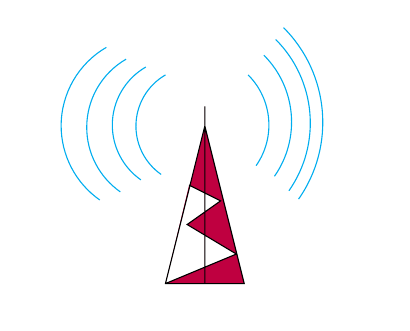
\begin{tikzpicture}[transform shape,scale=5]
			\clip (-0.9,-0.1) rectangle (0,.6);
			\begin{pgfinterruptboundingbox}
				%------------Cột phát
				\tikzset{cotphat/.pic={
						\begin{scope}
							\draw[fill=red!50!violet] (-1.45,-.1)--(-1.45,-.55) 
							(-1.55,-.55)--(-1.35,-.55)--(-1.45,-.15)--cycle
							(-1.49,-.3)--(-1.41,-.34)--(-1.495,-.4)--(-1.37,-.475)--(-1.55,-.55);
						\end{scope}
						\draw[cyan](-1.25,.1)arc(45:-35:.34 and .34);
						\draw[cyan](-1.27,.07)arc(45:-35:.3 and .3);
						\draw[cyan](-1.3,.03)arc(45:-35:.24 and .24);
						\draw[cyan](-1.34,-.02)arc(45:-35:.18 and .18);
						\draw[cyan](-1.7,.05)arc(120:235:.23 and .23);
						\draw[cyan](-1.65,.02)arc(120:235:.2 and .2);
						\draw[cyan](-1.6,0)arc(120:235:.17 and .17);
						\draw[cyan](-1.55,-0.02)arc(120:235:.15 and .15);
				}}
				\path pic[xshift=1cm,yshift=.5cm]{cotphat};
			\end{pgfinterruptboundingbox}
		\end{tikzpicture}
	}
	\loigiai{
		\begin{enumerate}
			\item Phương trình mặt cầu để mô tả ranh giới bên ngoài của vùng phủ sóng trong không gian là
			$$(x+3)^2+(y-2)^2+(z-7)^2=9.$$
			\item Ta có $\overrightarrow{IA}=(1;-1;1)$ nên $IA=\sqrt{1^2+(-1)^2+1^2}=\sqrt{3}<3$.\\
			Vì $IA<R$ nên điểm $A$ nằm trong mặt cầu. Vậy người dùng điện thoại ở điểm $A(-2;1;8)$ có thể sử dụng dịch vụ của trạm này.
			\item Ta có $\overrightarrow{IB} = (5;1;-3)$ nên $IB=\sqrt{5^2+1^2+(-3)^2}=\sqrt{35}>3$.\\
			Vì $IB>R$ nên điểm $B$ nằm ngoài mặt cầu. Vậy người dùng điện thoại ở điểm $B(2;3;4)$ không thể sử dụng dịch vụ của trạm này.
		\end{enumerate}
	}
\end{bt}

\begin{bt}%[2H5H3-3]
% nguon: Archive/2024/0. [LVH] BG - 12 New - 4in1-20240625T224301Z-001/0. [LVH] BG - 12 New - 4in1/data/data_C5/Bai-3-Dang-2-Vitrituongdoi.tex #1456
[KNTT]%[BG-12-New-4in1, Nguyễn Cường]
	Trong không gian $Oxyz$, cho mặt cầu $(S)$ có phương trình $$(x+2)^2+y^2+\left(z+\frac{1}{2}\right)^2=\frac{9}{4}.$$
	\begin{enumerate}
		\item Xác định tâm và bán kính của $(S)$.
		\item Hỏi điểm $M(2 ; 0 ; 1)$ nằm trong, nằm ngoài hay thuộc mặt cầu $(S)$?
	\end{enumerate}
	\loigiai{	
		\begin{enumerate}
			\item Ta viết lại phương trình của mặt cầu $(S)$ dưới dạng: $$\left[x-(-2)\right]^2+(y-0)^2+\left[x -\left(-\frac{1}{2}\right)\right]^2=\left(\dfrac{3}{2}\right)^2.$$ 
			Vậy mặt cầu $(S)$ có tâm $I\left(-2 ;0 ; -\dfrac{1}{2}\right)$ và bán kính $R=\dfrac{3}{2}$.
			\item Ta có $MI^2=(2+2)^2+(0+0)^2+\left(1+\dfrac{1}{2}\right)^2=\dfrac{73}{4}>\dfrac{3}{2}=R^2$.\\
			Do đó, điểm  $M(2 ; 0 ; 1)$ nằm ngoài mặt cầu $(S)$.
		\end{enumerate}
	}
\end{bt}

\begin{bt}%[2H5H3-3]
% nguon: Archive/2024/0. [LVH] BG - 12 New - 4in1-20240625T224301Z-001/0. [LVH] BG - 12 New - 4in1/data/data_C5/Bai-3-Dang-2-Vitrituongdoi.tex #1457
[CD]%[BG-12-New-4in1, Nguyễn Cường]
	Cho mặt cầu có phương trình $(x-1)^2+(y+2)^2+(z-7)^2=100$.
	\begin{enumerate}
		\item Xác định tâm và bán kính mặt cầu.
		\item Mỗi điểm $A(1;1;1)$, $B(9;4;7)$, $C(9;9;10)$ nằm trong, nằm ngoài hay nằm trên mặt cầu đó?
	\end{enumerate}
	\loigiai{
		\begin{enumerate}
			\item Mặt cầu có tâm $I(1;-2;7)$ và bán kính $R=10$.
			\item Ta có 
			\begin{itemize}
				\item $IA=\sqrt{(1-1)^2+(1+2)^2+(1-7)^2}=\sqrt{45}<R$ nên điểm $A$ nằm bên trong mặt cầu.
				\item $IB=\sqrt{(9-1)^2+(4+2)^2+(7-7)^2}=\sqrt{100}=R$ nên điểm $B$ nằm trên mặt cầu.
				\item $IC=\sqrt{(9-1)^2+(9+2)^2+(10-7)^2}=\sqrt{194}>R$ nên điểm $C$ nằm ngoài mặt cầu.
			\end{itemize}
		\end{enumerate}
	}
\end{bt}

\begin{bt}%[2H5H3-4]
% nguon: Archive/2024/0. [LVH] BG - 12 New - 4in1-20240625T224301Z-001/0. [LVH] BG - 12 New - 4in1/data/data_C5/Bai-3-Dang-2-Vitrituongdoi.tex #1458
[KNTT]%[BG-12-New-4in1, Nguyễn Cường]
	Trong không gian $Oxyz$, một thiết bị phát sóng đặt tại vị trí $A(2 ; 0 ; 0)$. Vùng phủ sóng của thiết bị có bán kính bằng $1$. Hỏi vị trí $M(2 ; 1 ; 1)$ có thuộc vùng phủ sóng của thiết bị nói trên hay không?
	\loigiai{
		Theo đề bài ta có thiết bị phủ sóng sẽ thuộc khối cầu tâm $A$ và bán kính $R = 1$, 
		suy ra trình mặt cầu là $(x-2)^2+y^2+z^2 = 1$.\\ 
		Ta có $AM = \sqrt{2} > R$.	Do vậy điểm $M$ không thuộc vùng phủ sóng.
	}
\end{bt}

\begin{bt}%[2H5V3-4]
% nguon: Archive/2024/0. [LVH] BG - 12 New - 4in1-20240625T224301Z-001/0. [LVH] BG - 12 New - 4in1/data/data_C5/Bai-3-Dang-2-Vitrituongdoi.tex #1459
[CKP]%[BG-12-New-4in1, Nguyễn Cường]
	Một sân hình chữ nhật $ABCD$ có chiều dài $AD=20$ m, chiều rộng $AB=15$ m. Người ta đặt một camera ở độ cao $5$ m trên một cây cột vuông góc với mặt sân tại $A$, biết camera có bán kính quan sát là $25$ m. Xét hệ trục toạ độ $Oxyz$ với gốc toạ độ $O$ trùng với điểm $A$ chân cột, các tia $Ox$, $Oy$ lần lượt chứa các cạnh $A B$, $AD$ của sân và tia $Oz$ chứa cây cột.
	\begin{center}
		\definecolor{brown(traditional)}{rgb}{0.59, 0.29, 0.0}
		\definecolor{darkpastelgreen}{rgb}{0.01, 0.75, 0.24}
		\begin{tikzpicture}[line join=round, line cap=round,scale=2,transform shape]
			%\clip (-3,-2.5) rectangle (3,2.5);
			\tikzset{san/.pic={
					\foreach \i in{0,1,2,3,4,5,6}{
						\draw[fill=brown(traditional)] (0+\i,-3.5)--(0+\i,-2)--(.2+\i,-1.7)--(.4+\i,-2)--(.4+\i,-3.5)--cycle
						;
						\draw[fill=brown(traditional)]  (-.5,-3.2) rectangle (7,-2.9)
						(-.5,-2.6) rectangle (7,-2.3);
					}
					
			}}
			\tikzset{co/.pic={
					
					\path 
					(-.6,.7) coordinate (A)
					(-2.8,-.5) coordinate (x)
					(2.85,-1.3) coordinate (y)
					(-.6,2) coordinate (z)
					($(A)!.85!(x)$) coordinate (B)
					($(A)!.9!(y)$) coordinate (D)
					($(B)+(D)-(A)$) coordinate (C)
					($(A)!.9!(x)$) coordinate (B')
					($(B')+(D)-(A)$) coordinate (C')
					($(A)!.1!(D)$) coordinate (E)
					($(B)!.1!(C)$) coordinate (F)
					;
					\foreach\p/\g in {A/-90,x/-90,y/-90, z/180, D/45, C/-45, B/140}
					\node at (\p) [shift=(\g:2mm)] {\tiny $\p$};
					\draw[->] (A)--(x) ; 
					\draw[->] (A)--(y);
					\draw[->] (A)--(z);
					\draw[fill=darkpastelgreen] (A)--(B)--(C)--(D);
					\draw[<->] (B')--(C') ; 
					\draw[<->] (E)--(F) ; 
					\draw[<->] (-1.8,.7)--(-1.8,1.6) ; 
					\draw[dashed] (-2,.7)--(-.6,.7) (-2,1.6)--(-.6,1.6) ; 
					\node at (-2.1,1.2) {\tiny $5$ m};
					\node at (-1,-1.5)[rotate=-30] {\tiny $20$ m};
					\node at (-.9,0)[rotate=30] {\tiny $15$ m};
					\node at (A) [below]{\tiny $A$};
			}}
			\path
			(0,0)pic[scale=1]{co}
			(.8,-1.3)pic[scale=.25,yslant=.6]{san}
			(-2.35,.75)pic[scale=.25,yslant=.6]{san}
			(1.5,.55)pic[xscale=-1,scale=.3,yslant=.6]{san}
			;
			\draw[fill=brown(traditional)]  
			(-.7,.7) rectangle (-.8,1.6);
			\draw[fill=brown(traditional)]  (-.7,.7)--(-.6,.8)--(-.6,1.7)--(-.7,1.6)--cycle
			(-.6,1.7)--(-.7,1.6)--(-.8,1.6)--(-.7,1.7)--cycle;
			\draw[fill=white,yslant=.3] (-.4,1.6) circle (1.8pt);
			\draw[fill=black,yslant=.3] (-.4,1.6) circle (.8pt);
			\draw (-.45,1.55)--(-.32,1.55)--(-.38,1.4)--(-.48,1.4)--cycle;
			\draw[fill=gray] (-.48,1.4)--(-.45,1.55)--(-.6,1.56)--(-.6,1.5)--cycle;
		\end{tikzpicture}
		
	\end{center}
	\begin{enumerate}
		\item Viết phương trình mặt cầu mô tả ranh giới bên ngoài và bên trong của vùng quan sát được.
		\item Hỏi camera có thể quan sát toàn bộ sân hay không? Vì sao?
	\end{enumerate}
	\loigiai{
		\begin{enumerate}
			\item Chọn hệ trục tọa độ $Oxyz$ với mỗi đơn vị độ dài trong hệ trục tương ứng với $1$ m trong thực tế.\\
			Mặt cầu mô tả ranh giới bên ngoài và bên trong của vùng quan sát được có tâm $ I(0;0;5) $, bán kính $ R=25 $.\\
			Vậy phương trình mặt cầu là $ x^2+y^2+(z-5)^2=25^2 \Leftrightarrow x^2+y^2+(z-5)^2=625$.
			\item Đặt $ f(x,y,z)=x^2+y^2+(z-5)^2 $.\\
			Xét các điểm $ A(0;0;0) $, $ B(15;0;0) $, $ C(15;20;0) $.\\
			Ta có $ f(A)=5^2=25<625 $, $ f(B)= 15^2+5^2=225<625$, $ f(C)=15^2+20^2+5^2=650>625 $.\\
			Suy ra $ A $, $ B $ nằm trong vùng quan sát được của camera; $ C $ không nằm trong vùng quan sát được của camera.\\
			Vậy camera không thể quan sát toàn bộ sân.
		\end{enumerate}	
	}
\end{bt}

\begin{bt}%[2H5V3-4]
% nguon: Archive/2024/TaiLieuGiangDay/5.HH Oxyz/VDC_TDM.tex #3164
%[Thành Đức Trung]
Trong không gian $Oxyz$, cho hai điểm $A(-2;4;2)$, $B(2;0;3)$ và mặt cầu $(S)\colon (x-1)^2+y^2+(z-2)^2=16$. Gọi $M$ là điểm chạy trên mặt cầu $(S)$. Hãy tìm giá trị nhỏ nhất của $P=AM+MB$ và giá trị lớn nhất của biểu thức $Q=MA-MB$.
\loigiai
{
\immini
{
Mặt cầu $(S)$ có tâm $I(1;0;2)$, bán kính $R=4$. \\
Ta có $IA=\sqrt{\left(1+2\right)^2+4^2+\left(2-2\right)^2}=5>R$, suy ra $A$ nằm ngoài $(S)$. \\
Ta có $IB=\sqrt{\left(1-2\right)^2+0^2+\left(2-3\right)^2}=\sqrt{2}$, suy ra $B$ nằm trong $(S)$. \\
Ta có $AB=\sqrt{\left(2+2\right)^2+\left(0-4\right)^2+\left(3-2\right)^2}=\sqrt{33}$.
}
{
\begin{tikzpicture}[scale=0.9, font=\footnotesize, line join=round, line cap=round, >=stealth]
\path
(0,0)coordinate(I)
(-4,1)coordinate(A)
(-0.5,0.5)coordinate(B)
(-1.17,1.62)coordinate(M)
(-1.87,0.7)coordinate(M_1)
(1.99,0.14)coordinate(M_2)
;
\draw
(I)circle(2cm)
(A)--(1.99,0.14)
(B)--(M)--(A)
;
\foreach \p/\q in {I/-90, A/180, B/90, M/135, M_1/-150, M_2/0} \fill[black] (\p) circle (2pt) ($(\p)+(\q:4mm)$) node{$\p$};
\end{tikzpicture}
}
\noindent
Gọi $M_1$ là giao điểm của đoạn thẳng $AB$ và mặt cầu $(S)$. \\
Ta có $P=AM+MB\geqslant AB=\sqrt{33}$. \\
Suy ra $P_{\min}=\sqrt{33}$ khi $M\equiv M_1$. \\
Gọi $M_2$ là giao điểm của tia đối tia $BA$ và mặt cầu $(S)$. \\
Ta có $Q=MA-MB\leqslant AB=\sqrt{33}$. \\
Suy ra $Q_{\max}=\sqrt{33}$ khi $M\equiv M_2$.
}
\end{bt}

\begin{bt}%[2H5C3-4]
% nguon: Archive/2024/TaiLieuGiangDay/5.HH Oxyz/VDC_TDM_Dot2.tex #3176

	Trong không gian $Oxyz$, cho mặt cầu $(S)\colon x^2+y^2+z^2-2 x-8=0$ và mặt phẳng $(\alpha)\colon x+2y-z-1=0$. Gọi $(C)$ là đường tròn giao tuyến của $(S)$ và $(\alpha)$. Gọi $M$ là điểm nằm trên $(C)$. Hãy tìm giá trị lớn nhất và giá trị nhỏ nhất tung độ của điểm $M$?
	\loigiai{
		Do $(C)$ là đường tròn giao tuyến của $(S)$ và $(\alpha)$ nên ta có $(C)\colon\heva{&x^2+y^2+z^2-2 x-8=0\\&x+2y-z-1=0.}$ \\
		Suy ra với mọi $M(x;y;z)\in (C)$ ta có 
		$x^2+y^2+(x+2y-1)^2-2x-8=0$ \\
		hay $2x^2+4x(y-1)+5y^2-4y-7=0$ (*). \\
		Do $M\in (C)$ nên phương trình (*) có nghiệm $x$. \\
		Suy ra 
		$4(y-1)^2-2\cdot \left(5y^2-4y-7\right)\ge 0\Leftrightarrow -6y^2+18\ge 0\Leftrightarrow -\sqrt{3}\le y\le \sqrt{3}$. \\
		Vậy tung độ lớn nhất và nhỏ nhất của của các điểm $M$ lần lượt là $\sqrt{3}$ và $-\sqrt{3}$.
	}
\end{bt}

\begin{bt}%[2H5C2-6]
% nguon: Archive/2024/TaiLieuGiangDay/5.HH Oxyz/VDC_TDM_Dot2.tex #3177

Trong không gian $Oxyz$, cho mặt cầu $(S)\colon  (x+2)^2 +(y-2)^2+(z-1)^2=21$ và hai mặt phẳng $
(\alpha)\colon  3x -y - z -2  = 0$,  $(\beta)\colon -2x + y +4z -19  = 0.$ 
Gọi $(C)$ là đường tròn giao tuyến của $(S)$ và $(\alpha)$. Gọi $M$ là điểm chạy trên $(C)$ và $N$ là điểm chạy trên $(\beta)$. 
Hãy xác định khoảng cách $MN$ nhỏ nhất và xác định tọa độ $M$, $N$?
\loigiai{
\immini{Ta có $(S)\colon \heva{& \text{tâm } I(-2;2;1)\\ &R=\sqrt{21}.}$\\
Đường tròn giao tuyến $(C)$ có tâm $J $ là hình chiếu của $I$ lên $(\alpha)$ và bán kính $r=\sqrt{R^2 - \mathrm {d}^2 (I, (\alpha))}$.\\
Trong đó $\mathrm d(I, (\alpha ))=\dfrac{|3\cdot (-2) -2 -1-2|}{\sqrt{9+ 1+ 1}}=\sqrt{11}$. Suy ra $r = \sqrt{10}$.\\
Ta có $IJ \colon \heva{& x= -2 + 3t\\ & y= 2-t \\&z=1-t}$ ($t \in \mathbb{R}$).}{	\begin{tikzpicture}[scale=0.7]
	
	% Lưới ô vuông (tuỳ chọn)
	\draw[step=1cm,gray!30,very thin] (-2,-1) grid (10,7);
	% Mặt phẳng alpha (hình bình hành dưới)
	\coordinate (A) at (-1,0);
	\coordinate (B) at (6,0);
	\coordinate (C) at (8,3);
	\coordinate (D) at ($(A)-(B)+(C)$);
	\coordinate (J) at (3,1.5);
	\coordinate (H) at (7,1.5);
	\coordinate (N) at (6,4);
	\draw[thick] (A) -- (B) -- (C) -- (D) -- cycle;
	\path[name path=JH] (J)--(H);
	% Elip nằm trong mặt phẳng alpha
	\draw[name path=elip, thick] (J) ellipse (2cm and 0.6cm);
	\path[name intersections={of=JH and elip, by=M}];
	
	% Mặt phẳng beta (hình thoi dựng đứng)
	\coordinate (F) at (5,4);
	\coordinate (E) at ($(C)-(B)+(F)$);
	\draw pic[draw,angle radius=2mm] {right angle = M--H--B}; B
	\draw pic[draw,angle radius=2mm] {right angle = M--N--H}; 
	\draw[thick] (B) -- (F) -- (E) -- (C);
	\draw[dashed, red] (J)--(H) (M)--(N);
	\foreach \p/\r in {J/8-90,H/0, M/-80, N/0}
	\fill (\p) circle (1.5pt) node[shift={(\r:3mm)}]{$\p$};
	\end{tikzpicture}}
\noindent	Suy ra $J(-2+3t; 2- t; 1-t)$. Mà $J \in (\alpha)$ nên $$3\cdot (-2+ 3t) - (2-t)-(1-t)-2=0 \Leftrightarrow t= 1.$$
\noindent Suy ra $J(1;1;0)$.\\
Gọi $d$ là giao tuyến của hai mặt phẳng $(\alpha)$ và $(\beta)$. Suy ra $d \colon \heva{& x= 3 + 3t \\ &y=1 +10t \\&z=6-t}$ ($ t \in \mathbb{R}$).\\
Gọi  $H$ là hình chiếu của $J$ lên $d$. 
Khi đó $MN$ ngắn nhất khi và chỉ khi $M$ là  giao điểm của đoạn thẳng $JH$ với $(C)$ và $N$ là hình chiếu của $M$ lên $(\beta)$.\\
Gọi $H(3+ 3t; 1+10t ; 6-t) \in d$.\\
Do  $\vec{JH} \perp \vec{u} $, với $\vec{u}= (3;10;-1)$ là một véc-tơ chỉ phương của $d$, nên $$ 3 \cdot (3t+2) +10 \cdot 10t  - 1 \cdot (6 - t)=0 \Leftrightarrow t= 0 \Rightarrow H \left(3;1; 6 \right).$$
\noindent 
Mặt khác $\vec{JM}= \dfrac{JM}{JH} \cdot \vec{JH}= \dfrac{\sqrt{10}}{\sqrt{\left( 3-1\right)^2+(1-1)^2)+ (6-0)^2   }} \cdot \vec{JN}$.\\
Suy ra $\vec{JM}= \dfrac{1}{2} \cdot \vec{JH} \Rightarrow M \left(2;1;3 \right)$.\\
Ta có $NM \colon \heva{& x= 2 -2t \\& y= 1+t \\ &z = 3 + 4t} $ ($t \in \mathbb{R}$).\\
Suy ra $N(2-2t;1+t ; 3+4t )\in (\beta) \Rightarrow -2\cdot (2-2t) + 1+t + 4\cdot (3+4t)-19=0 \Rightarrow t=\dfrac{10}{21}.$\\  Vậy $N\left(\dfrac{22}{21};\dfrac{31}{21};\dfrac{103}{21}\right)$ và độ dài ngắn nhất của $MN$ là $\mathrm d(M, (\beta))= \dfrac{|-2 \cdot 2 +1 + 4 \cdot 3-19|}{\sqrt{4+1+ 16}}= \dfrac{10\sqrt{21}}{21}$.}
\end{bt}

\begin{bt}%[2H5C1-5]
% nguon: Archive/2024/TaiLieuGiangDay/5.HH Oxyz/VDC_TDM_Dot2.tex #3179

	Trong không gian $O x y z$, cho ba điểm $A(1 ; 2 ; 0)$, $B(-1 ; 4 ; 2)$, $M(2 ; 2 ;-1)$. Hãy lập phương trình mặt phẳng $(P)$ đi qua $M$ sao cho biểu thức $T=\mathrm{d}(A,(P))+\mathrm{d}(B,(P))$ đạt giá trị lớn nhất?
	\loigiai{
		Gọi phương trình mặt phẳng $(P)$ có dạng $Ax+By+Cz+D=0$, (với $A^2+B^2+C^2=1$).\\
		Ta có $M(2;2;-1)\in (P)$ nên ta có $2A+2B-C+D=0\Rightarrow D=C-2A-2B$.\\
		Khi đó $(P)\colon Ax+By+Cz+C-2A-2B=0$.\\
		Ta có 
		\begin{eqnarray*}
			T=\mathrm{d}(A,(P))+\mathrm{d}(B, (P))&=& |A+2B+C-2A-2B|+|-A+4B+2C+C-2A-2B|\\
			&=& |-A+C|+|-3A+2B+3C|.
		\end{eqnarray*}
		\begin{itemize}
			\item $A$, $B$ nằm cùng phía mặt phẳng $(P)$ khi 
			\begin{eqnarray*}
				&&\left(Ax_A+By_A+Cz_A+D\right)\left(A x_B+B y_B+C z_B+D\right)>0\\
				&\Rightarrow& (-A+C)(-3A+2B+3C)>0. \quad (1)
			\end{eqnarray*}
			Khi đó \begin{eqnarray*}
				T&=&|-A+C-3A+2B+3C|\\
				&=&|-4A+2B+4C|\\
				&\leq& \sqrt{((-4)^2+2^2+4^2)(A^2+B^2+C^2)}\\
				&=& 6.
			\end{eqnarray*}
			\item   $A$, $B$ nằm khác phía mặt phẳng $(P)$
			khi
			$A$, $B$ nằm cùng phía mặt phẳng $(P)$ khi
			\begin{eqnarray*}
				&&\left(Ax_A+By_A+Cz_A+D\right)\left(A x_B+B y_B+C z_B+D\right)<0\\
				&\Rightarrow& (-A+C)(-3A+2B+3C)<0. \quad (2)
			\end{eqnarray*}
			Khi đó 
			\allowdisplaybreaks
			\begin{eqnarray*}
				T&=&|-A+C+3A-2B-3C|\\
				&=&|2A-2B-2C|\\
				&\leq&\sqrt{(2^2+(-2)^2+(-2)^2)(A^2+B^2+C^2)}\\
				&=&2\sqrt{3}.
			\end{eqnarray*}
		\end{itemize}
		So sánh hai giá trị lớn nhất của $T$, ta nhận thấy $\max T=6$.\\
		Dấu \lq\lq$=$\rq\rq\, xảy ra khi $\dfrac{A}{-4}=\dfrac{B}{2}=\dfrac{C}{4}=k$.\\
		Thay $A=-4k$, $B=2k$, $C=4k$ vào $A^2+B^2+C^2=1$ ta được
		$$16k^2+4k^2+16k^2=1\Rightarrow k=\pm \dfrac{1}{6}.$$
		Với $k=\dfrac{1}{6}$, ta kiểm tra $(1)$ (đúng).\\
		Với $k=-\dfrac{1}{6}$, ta kiểm tra $(1)$ (đúng).\\
		Dễ thấy $k=\pm \dfrac{1}{6}$ thì $\max T=6$ nên ta chọn $A=-\dfrac{2}{3}$, $B=\dfrac{1}{3}$, $C=\dfrac{2}{3}$.\\
		Vậy $(P)\colon -\dfrac{2}{3}x+\dfrac{1}{3}y+\dfrac{2}{3}z+\dfrac{4}{3}=0$.
	}
\end{bt}

\begin{bt}%[2H5H1-3]
% nguon: Archive/SP_KhoLatex/ID6_old/2-GHK2-17-THPTSo3BaoThang-LaoCai-22TN-TL.tex #3591
%[GHK2 THPT Số 3 Bảo Thắng - Lào Cai, 2022]%[Phan Quốc Trí, 12EX4-2022]
	Trong không gian $Oxyz$, cho ba điểm $A(0;1;2)$, $B(2;0;3)$ và $C(3;4;0)$. Viết phương trình mặt phẳng $(ABC)$.
	\loigiai{
		Ta có 	$\overrightarrow{AB}=(2;-1;1)$, $\overrightarrow{AC}=(3;3;-2)$ và $\left[\overrightarrow{AB},\overrightarrow{AC} \right]=\left(-1;7;9\right)$.\\
		Mặt phẳng $(ABC)$ đi qua điểm $A(0;1;2)$, có véc-tơ pháp tuyến $\overrightarrow{n}=\left(-1;7;9\right)$ nên có phương trình
		$$-x +7(y-1) +9(z-2) =0 \Leftrightarrow -x+7y+9z-25=0.$$
	}
\end{bt}

\begin{bt}%[2H5H1-3]
% nguon: Archive/SP_KhoLatex/ID6_old/2-GHK2-24-HuongHoa-QuangTri-22.tex #3649
%[Đề thi GHK2 - THPT Hướng Hóa, Quảng Trị - 2022]%[Hoàng Thanh Phương - 12-EX4]
	Trong không gian với hệ tọa độ $Oxyz$, cho hai điểm $A(2;0;-1)$, $B(1;-1;3)$, mặt phẳng $(P)\colon 3x+2y-z+5=0$. Viết phương trình mặt phẳng $(\alpha)$ đi qua hai điểm $A$, $B$ và vuông góc với mặt phẳng $(P)$.
\loigiai{
Vì $(\alpha)\perp (P)$ nên $\overrightarrow{n}_{(\alpha)}\perp \overrightarrow{n}_{(P)}$. \quad (1) \\
Mặt khác, $(\alpha)$ đi qua hai điểm $A$ và $B$ nên $\overrightarrow{n}_{(\alpha)}\perp \overrightarrow{AB}$. \quad (2) \\
Từ $(1)$ và $(2)$, ta có $[\overrightarrow{AB}, \overrightarrow{n}_{(P)}]$ là một véc-tơ pháp tuyến của mặt phẳng $(\alpha)$. \\
Ta có $[\overrightarrow{AB}, \overrightarrow{n}_{(P)}]=(-7;11;1)$. \\
Phương trình mặt phẳng $(\alpha)$ là
$$-7(x-2)+11y+(z+1)=0\Leftrightarrow -7x+11y+z+15=0.$$ 
}
\end{bt}

\begin{bt}%[2H5V1-3]
% nguon: Archive/SP_KhoLatex/ID6_old/2-GHK2-25-TXQuangTri-QuangTri-22.tex #3733
%[Thi giữa học kỳ 2- THPT TX Quảng Trị- Quảng Trị - 22]%[Lê Văn Toàn - EX4]
	Trong không gian $Oxyz$, viết phương trình mặt phẳng qua $A(1;2;3)$ và vuông góc với hai mặt phẳng $(P)\colon 3x-2y+z+4=0$, $(Q)\colon 5x-4y+3z+1=0$.	
	\loigiai{
	Gọi $(\alpha)$ là mặt phẳng cần tìm và $\overrightarrow{n}_{(\alpha)}$ là một véc-tơ pháp tuyến của mặt phẳng $(\alpha)$.\\
	Mặt phẳng $(P)\colon 3x-2y+z+4=0$ có véc-tơ pháp tuyến $\overrightarrow{n}_{P}=(3;-2;1)$; mặt phẳng $(Q)\colon 5x-4y+3z+1=0$ có véc-tơ pháp tuyến $\overrightarrow{n}_{Q}=(5;-4;3)$.\\
	Suy ra $\overrightarrow{n}_{(\alpha)}=\left[\overrightarrow{n}_{P};\overrightarrow{n}_{Q}\right]=(-2;-4;-2)$.\\
	Mặt phẳng $(\alpha)$ qua $A$ có véc-tơ pháp tuyến $\overrightarrow{n}_{(\alpha)}$ nên có phương trình là
	$$(\alpha)\colon -2(x-1)-4(y-2)-2(z-3)=0 \Leftrightarrow -2x-4y-2z+16=0 \Leftrightarrow x+2y+z-8=0.$$
}
	\end{bt}

\begin{bt}%[2H5H1-3]
% nguon: Archive/SP_KhoLatex/ID6_old/2-GHK2-19-THPTTanBinh-HCM-22.tex #3753
%[2-GHK2-19-THPTTanBinh-HCM-22]%[Lương Như Quỳnh, 12-EX4-2022]
	Trong không gian $ Oxyz $, viết phương trình mặt phẳng $ (P) $ đi qua hai điểm $ A(1;2;0) $, $ B(2;3;1) $ và song song với $ Ox $.
	\loigiai{
	Ta có $ \overrightarrow{AB}=(1;1;1) $; $ \overrightarrow{n}=\left[ \overrightarrow{AB},\overrightarrow{i}\right]=(0;1;-1)$.\\
	Phương trình mặt phẳng $ (P) $ đi qua hai điểm $ A(1;2;0) $ và nhận $ \overrightarrow{n}$ là một véc-tơ pháp tuyến là 
	\[0(x-1)+1(y-2)-1(z-0)=0\Leftrightarrow y-z-2=0.\]
	}	
\end{bt}

\begin{bt}%[2H5H2-8]
% nguon: Archive/SP-4Phan-Dot3/Data/CD_2-OTHK2-De05.tex #4378
%[Dự án Đề thi 4 phần-Đợt 3]%[Đắc Vũ]
	Trong không gian $Oxyz$, một cabin cáp treo xuất phát từ điểm $A(10;3;0)$ và chuyển động đều theo đường cáp có véc-tơ chỉ phương là $\overrightarrow{u}=(2;-2;1)$ với tốc độ là $4{,}5$ m/s (đơn vị trên mỗi trục tọa độ là mét). Sau thời gian $180$ giây, Cabin dừng ở điểm $B$. Tìm tọa độ điểm $B$.
	\begin{center}
		\begin{tikzpicture}[line join=round,line cap=round,>=stealth,scale=0.75,font=\footnotesize]
			\tikzset{every node/.style={outer sep=-0.5mm}}
			\foreach \x/\y/\n in {0/0/O,5/0/y,0/4/z,-4/-4/x,-5/2.5/B} \coordinate (\n) at (\x,\y);
			\coordinate (C) at ($(O)!0.1!(y)$);
			\coordinate (D) at ($(O)!0.15!(x)$);
			\coordinate (A) at ($(C)+(D)-(O)$);
			\coordinate (E) at ($(O)!0.8!(x)$);
			\coordinate (M) at ($(A)!0.65!(B)$);
			\coordinate (v) at ($(A)!0.15!(B)$);
			\coordinate (u) at ($(O)+(v)-(A)$);
			\draw[->] (O)--(x) node[right] {\normalsize$x$};
			\draw[->] (O)--(y) node[below left] {\normalsize$y$};
			\draw[->] (O)--(z) node[below left] {\normalsize$z$};
			\draw[dashed,thin](C)--(A)--(D) (B)node[above]{$B$}--(E)node[below right]{$550$};
			\draw (E) node[left]{$x_B$};
			\draw (O) node[above right]{$O$};
			\draw (C) node[below]{$3$};
			\draw (D) node[left]{$10$};
			\fill (A) circle (1.5pt) node[below right] {$A(10;3;0)$};
			\draw[very thick] (A)--(B);
			\draw[->,very thick,red] (O)--(u)node[above]{$\overrightarrow{u}$};
			\fill[red] (M) circle (2pt) node[above right] {$M$};
			\draw (M) .. controls ($(M)+(-0.2,-0.1)$) .. ($(M)+(0,-0.2)$) node[below,yshift=1mm]{{\large \faCube}};
			\draw ($(O)+(0,-4)$); %node[below]{\textit{Hình 35}};
		\end{tikzpicture}
	\end{center}
	\loigiai{
		Phương trình tham số của đường cáp là $\heva{&x=10+2t\\ &y=3-2t\\ &z=t}$ với $t\ge 0$.\\
		Sau $180$ giây, ta có $AB=4{,}5\cdot 180 =810$ mét.\\
		Gọi $B(10+2t;3-2t;t)$. \\
		Ta có $AB=810 \Leftrightarrow \sqrt{(2t)^2+(-2t)^2+t^2}=810 \Leftrightarrow 3t=810 \Leftrightarrow t=270$.\\
		Vậy $B(550;-537;270)$.
	}
\end{bt}

\begin{bt}%[2H5H3-4]
% nguon: Archive/SP-4Phan-Dot3/Data/CD_2-OTHK2-De05.tex #4380
%[Dự án Đề thi 4 phần-Đợt 3]%[Đắc Vũ]
	Trong không gian $Oxyz$ cho trước (đơn vị trên trục là mét), một trạm thu phát sóng $5$G có bán kính vùng phủ sóng của trạm ở ngưỡng $600$ m được đặt ở vị trí $I(200 ; 450 ; 60)$. Một người đang dùng điện thoại đang ở vị trí $M(a ; a ; 60)$. Hỏi có bao nhiêu vị trí điểm $M$ để người dùng điện thoại có thể nằm trong vùng phủ sóng của trạm dịch vụ này. Biết $M$ có tọa độ là những số nguyên dương.
	\loigiai{
		Phương trình mặt cầu $(S)$ mô tả ranh giới bên ngoài và bên trong của vùng phủ sóng có tâm $I( 200;450;60 )$ bán kính $ r=600$, có phương trình là 
		\[(S) \colon ( x-200 )^2+( y-450 )^2+( z-60 )^2=600^2.\]
		Để điểm $M$ nằm trong vùng phủ sóng của trạm dịch vụ thì
		\[IM \le 600 \Leftrightarrow \left(a-200\right)^2+(a-450)^2\le 600^2 \Leftrightarrow 2a^2-1\,300 a - 117\,500 \le 0.\]
		$\Rightarrow -80{,}4  \le a \le 730{,}4 \Rightarrow a\in\{1;2;3;\cdots;730\}$.\\
		Vậy có $730$ vị trí điểm $M$ thỏa yêu cầu.		
	}
\end{bt}

\begin{bt}%[2H5V3-4]
% nguon: Archive/SP-4Phan-Dot3/Data/CD_2-OTHK2-De01.tex #4420
%[Dự án đè thi 4 phần đợt 3]%[Trần Xuân Hòa]
	\immini[thm]{
		Người ta muốn thiết kế một quả địa cầu trong không gian $Oxyz$ bằng phần mềm 3D. Biết phương trình mặt cầu là $$(S)\colon (x-24)^2+(y-24)^2+(z-24)^2=100$$ và phương trình đường thẳng trục xoay là $$d\colon \dfrac{x-24}{1}=\dfrac{y-24}{1}=\dfrac{z-24}{3{,}25}.$$ 
	}
	{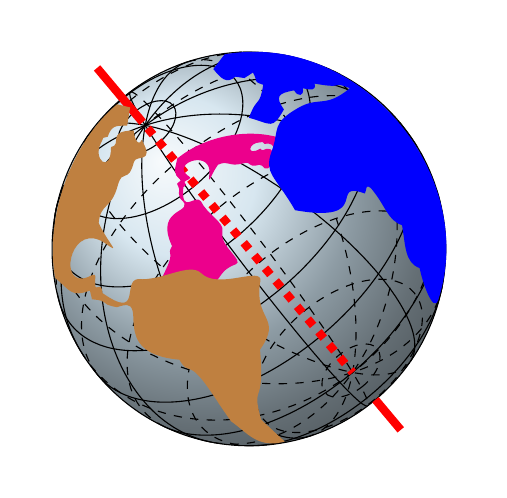
\begin{tikzpicture} [rotate=40] % "THE GLOBE"
			\newcommand\pgfmathsinandcos[3]{%
				\pgfmathsetmacro#1{sin(#3)}%
				\pgfmathsetmacro#2{cos(#3)}%
			}
			\newcommand\LongitudePlane[3][current plane]{%
				\pgfmathsinandcos\sinEl\cosEl{#2} % elevation
				\pgfmathsinandcos\sint\cost{#3} % azimuth
				\tikzset{#1/.style={cm={\cost,\sint*\sinEl,0,\cosEl,(0,0)}}}
			}
			\newcommand\LatitudePlane[3][current plane]{%
				\pgfmathsinandcos\sinEl\cosEl{#2} % elevation
				\pgfmathsinandcos\sint\cost{#3} % latitude
				\pgfmathsetmacro\yshift{\cosEl*\sint}
				\tikzset{#1/.style={cm={\cost,0,0,\cost*\sinEl,(0,\yshift)}}} %
			}
			\newcommand\DrawLongitudeCircle[2][1]{
				\LongitudePlane{\angEl}{#2}
				\tikzset{current plane/.prefix style={scale=#1}}
				% angle of "visibility"
				\pgfmathsetmacro\angVis{atan(sin(#2)*cos(\angEl)/sin(\angEl))} %
				\draw[current plane] (\angVis:1) arc (\angVis:\angVis+180:1);
				\draw[current plane,dashed] (\angVis-180:1) arc (\angVis-180:\angVis:1);
			}
			\newcommand\DrawLatitudeCircle[2][1]{
				\LatitudePlane{\angEl}{#2}
				\tikzset{current plane/.prefix style={scale=#1}}
				\pgfmathsetmacro\sinVis{sin(#2)/cos(#2)*sin(\angEl)/cos(\angEl)}
				% angle of "visibility"
				\pgfmathsetmacro\angVis{asin(min(1,max(\sinVis,-1)))}
				\draw[current plane] (\angVis:1) arc (\angVis:-\angVis-180:1);
				\draw[current plane,dashed] (180-\angVis:1) arc (180-\angVis:\angVis:1);
			}
			
			%% document-wide tikz options and styles
			
			\tikzset{%
				>=latex, % option for nice arrows
				inner sep=0pt,%
				outer sep=2pt,%
				mark coordinate/.style={inner sep=0pt,outer sep=0pt,minimum size=3pt,
					fill=black,circle}%
			}
			\def\N{
				(-.2,4.87)
				..controls +(180:1.52) and +(60:1.5) ..(-4.16,2.55)
				..controls +(-80:.5) and +(160:.5) ..(-3.7,1.75) --(-3.8,1.55)
				..controls +(-45:.5) and +(130:.5) ..(-3.45,1)
				..controls +(-20:1) and +(135:1.9) ..(-3.1,-1)
				..controls +(-100:.5) and +(85:.9) ..(-3,-2)
				..controls +(-95:.5) and +(85:.7) ..(-3.1,-3)
				..controls +(-75:.5) and +(155:.7) ..(-2.4,-4.25) --(-2.5,-3.45)
				..controls +(65:1) and +(-125:1.5) ..(-1.4,-2.1)
				..controls +(15:1) and +(-140:1) ..(-.3,-.8)
				..controls +(40:.4) and +(-85:.6) ..(-1.3,.3)
				..controls +(95:.4) and +(-45:.6) ..(-2.6,1.2)
				..controls +(145:.4) and +(-75:1.2) ..(-3.5,1.5)
				..controls +(55:.4) and +(-135:.5) ..(-3.4,1.9)
				..controls +(45:.2) and +(-35:.2) ..(-3.65,2.1)
				..controls +(145:.6) and +(105:1) ..(-2.65,2.4)
				..controls +(-75:.5) and +(-105:.6) ..(-2.45,2.9)
				..controls +(45:.5) and +(-145:.6) ..(-1.5,3.3)
				..controls +(35:.5) and +(-145:.6) ..(-.8,3.5)
				..controls +(35:.2) and +(-100:.7) ..(-.3,3.8)
				..controls +(-150:.2) and +(-130:.2) ..(-.3,4.1)
				..controls +(140:.7) and +(-30:.3) ..(-1,4.15)
				..controls +(-130:.7) and +(-160:.5) ..(-1.1,4.4)--(-1,4.45)--(-.9,4.4)
				..controls +(30:.3) and +(140:.3) ..(-.35,4.3)--(0,4.6)--cycle
				;
			}
			\def\M{
				(2.65,4.1)
				..controls +(-30:3.4) and +(32:3.3) ..(2.8,-4)
				..controls +(-148:.4) and +(-120:.3) ..(2.95,-3.1)
				..controls +(120:.4) and +(-120:.5) ..(3.3,-2)
				..controls +(120:.4) and +(-90:.6) ..(3.3,-.8)
				..controls +(100:.2) and +(20:.1) ..(3.1,-.8)
				..controls +(120:1) and +(-50:2) ..(1.5,0)
				..controls +(80:1) and +(-150:.6) ..(2,1.5)
				..controls +(30:.6) and +(170:.8) ..(3.2,1.9) %(4,1.5)
				..controls +(-10:.6) and +(180:.8) ..(4.5,1.45)
				..controls +(120:.6) and +(-50:.9) ..(3.9,2.1)
				..controls +(-120:.2) and +(-50:.2) ..(3.6,2.2)
				..controls +(-120:.2) and +(-100:.2) ..(3.4,2.3)
				..controls +(150:.4) and +(85:.4) ..(2.9,2.1)
				..controls +(-160:.6) and +(-55:.6) ..(2.1,2.5)
				..controls +(30:.6) and +(-140:.6) ..(2.9,2.9)
				..controls +(120:.3) and +(-100:.3) ..(2.9,3.3)--(2.65,3.33)--(2.5,3.5)
				..controls +(180:.3) and +(-90:.3) ..(2.2,4)--cycle
				;
			}
			\def\R{2.5} % sphere radius
			\def\angEl{35} % elevation angle
			\filldraw[ball color=blue!40!white!80!green!40!] (0,0) circle (\R);
			\foreach \t in {-80,-60,...,80} { \DrawLatitudeCircle[\R]{\t} }
			\foreach \t in {-5,-35,...,-175} { \DrawLongitudeCircle[\R]{\t} }
			\draw[line width=3pt,red, dashed](0,2)--(0,-2.05);
			\draw[line width=3pt,red](0,2.1)--(0,3) (0,-2.5)--(0,-3);
			\fill[magenta,scale=0.3,rotate=-60]\N;
			\fill[brown,scale=0.51] \N;
			\fill[blue,scale=0.51] \M;
		\end{tikzpicture}
	}	
	\noindent
	Gọi $M(a;b;c)$ là một giao điểm của $d$ và $(S)$, (biết $a>25$). Tính $T=a+b+c$. (Kết quả làm tròn đến hàng phần chục).
	\loigiai{
		Đường thẳng $d$ có phương trình tham số $\heva{&x=24+t\\&y=24+t\\&y=24+3{,}25t.}$\\
		Gọi $M$ là giao điểm của $d$ và $(S)$. Vì $M\in d$ nên $M(24+t;24+t;24+3{,}25t)$.\\
		Do $M\in (S)$ nên $$(24+t-24)^2+(24+t-24)^2+(24+3{,}25t-24)^2=100\Leftrightarrow t=\pm \dfrac{40\sqrt{201}}{201}.$$
		Vậy $d$ cắt $(S)$ tại hai điểm $M\left(24+\dfrac{40\sqrt{201}}{201};24+\dfrac{40\sqrt{201}}{201};24+\dfrac{130\sqrt{201}}{201}\right)$\\
		hoặc $N\left(24-\dfrac{40\sqrt{201}}{201};24-\dfrac{40\sqrt{201}}{201};24-\dfrac{130\sqrt{201}}{201}\right)$.\\
		Vậy $a+b+c=24+\dfrac{40\sqrt{201}}{201}+24+\dfrac{40\sqrt{201}}{201}+24+\dfrac{130\sqrt{201}}{201}\approx 86{,}8$.
	}
\end{bt}

\begin{bt}%[2H5V1-3]
% nguon: Archive/SP-4Phan-Dot3/Data/CD_2-OTGK2-De04.tex #4443
%[Dự án đề 4 phần]%[Đoàn Hùng]
	Trong không gian $Oxyz$, cho điểm $M(1;2;3)$. Mặt phẳng $(P)\colon ax+by+cz-14=0$ đi qua $M$ và cắt các trục tọa độ $Ox$, $Oy$, $Oz$ lần lượt tại các điểm $A$, $B$, $C$ không trùng với gốc tọa độ sao cho $M$ là trực tâm tam giác $ABC$. Tính giá trị biểu thức $S=2a+3b-4c$.
	\loigiai{
		Gọi $A(a;0;0)$, $B(0;b;0)$, $C(0;0;c)$ với $a, b, c\neq 0$. \\
		Phương trình mặt phẳng $(P)$ đi qua ba điểm $A$, $B$, $C$ là $\dfrac{x}{a}+\dfrac{y}{b}+\dfrac{z}{c}=1$.\\
		Do $M\in (P)$ nên $\dfrac{1}{a}+\dfrac{2}{b}+\dfrac{3}{c}=1.$\\
		Mặt khác, $M$ là trực tâm tam giác $ABC$ nên 
		\begin{align*}
			\heva{& AM\perp BC \\ & BM\perp AC}  \Leftrightarrow \heva{& \overrightarrow{AM}\cdot \overrightarrow{BC} =0 \\ & \overrightarrow{BM}\cdot \overrightarrow{AC}=0.}
		\end{align*}
		Lại có $\overrightarrow{AM}=(1-a;2;3)$, $\overrightarrow{BC}=(0;-b;c)$, $\overrightarrow{BM}=(1;2-b;3)$ và $\overrightarrow{AC}=(-a;0;c)$. 
		Khi đó
		\begin{align*}
			\heva{& -2b+3c=0 \\ & -a+3c=0 \\ &  \dfrac{1}{a}+\dfrac{2}{b}+\dfrac{3}{c}=1 }  \Leftrightarrow \heva{ & b=\dfrac{3}{2}c \\ & a=3c \\  & \dfrac{1}{3c}+\dfrac{4}{3c}+\dfrac{3}{c}=1}
			\Leftrightarrow \heva{& a=14 \\ & b=7 \\ & c=\dfrac{14}{3}.}
		\end{align*}
		Suy ra $(P)\colon \dfrac{x}{14}+\dfrac{y}{7}+\dfrac{3z}{14}=1 \Leftrightarrow x+2y+3z-14=0$.
		\\ Vậy $a=1$, $b=2$, $c=3$ và $S=-4$.
	}
\end{bt}

\begin{bt}%[2H5H2-5]
% nguon: Archive/SP-4Phan-Dot3/Data/KNTT_2-OTHK2_De01.tex #4448 
% KIEM_TRA: cần xem lại đáp số/dạng
%[Dự án soạn đề dự án đề GHK, HK 4 phần, Huỳnh Xuân Tín]
	Trong không gian với hệ tọa độ $Oxyz$, cho đường thẳng $d\colon  \heva{&x=5+t\\ &y=-2+t\\ &z=4+\sqrt{2}t},\, (t\in\mathbb{R})$ và mặt phẳng $(P)\colon x-y+\sqrt{2}z-7=0$. Hãy tính $\cos$ của góc giữa đường thẳng $d$ và mặt phẳng $(P)$.
	\loigiai{
		Đường thẳng $d$ có véc-tơ chỉ phương $\overrightarrow{u}(1;1;\sqrt{2})$.\\
		Mặt phẳng $(P)$ có véc-tơ pháp tuyến $\overrightarrow{n}(1;-1;\sqrt{2})$.\\
		Gọi $\varphi$ là góc giữa đường thẳng và mặt phẳng, khi đó ta có
		$$\sin\varphi=\dfrac{|\overrightarrow{u}\cdot\overrightarrow{n}|}{|\overrightarrow{u}|\cdot|\overrightarrow{n}|}=\dfrac{|1\cdot1+1\cdot(-1)+\sqrt{2}\cdot\sqrt{2}|}{\sqrt{1^2+1^2+\sqrt{2}^2}\cdot\sqrt{1^2+(-1)^2+\sqrt{2}^2}}=\dfrac{1}{2}.$$
		Từ đó suy ra $\varphi=30^\circ$.\\
		Vậy $\cos\varphi=\cos 30^\circ\approx 0{,}87$.
	}
\end{bt}

\begin{bt}%[2H5C1-7]
% nguon: Archive/SP-4Phan-Dot3/Data/CD_2-OTGK2-De01.tex #4454

	Một phần sân nhà bác An có dạng hình thang $ABCD$ vuông tại $A$ và $B$ với độ dài $AB=9$ m, $AD=5$ m và $BC=6$ m như Hình 5.9. Theo thiết kế ban đầu thì mặt sân bằng phẳng và $A$, $B$, $C$, $D$ có độ cao như nhau. Sau đó bác An thay đổi thiết kế để nước có thể thoát về phía góc sân ở vị trí $C$ bằng cách giữ nguyên độ cao ở $A$, giảm độ cao của sân ở vị trí $B$ và $D$ xuống thấp hơn độ cao ở $A$ lần lượt là $6$ cm và $3{,}6$ cm. Để mặt sân sau khi lát gạch vẫn là bề mặt phẳng thì bác An cần phải giảm độ cao ở $C$ xuống bao nhiêu cm so với độ cao ở $A$? (kết quả làm tròn đến hàng phần chục).
	\begin{center}
		\begin{tikzpicture}[scale=0.5, font=\footnotesize,line join=round, line cap=round, >=stealth]
			\path
			(0,0) coordinate (A) 
			(9,0) coordinate(B)
			(9,-6) coordinate(C)
			(0,-5) coordinate(D)
			;
			\draw[thick] (A)--(B)--(C)--(D)--cycle;
			\node [above] at ($(A)!0.5!(B)$) {$9$ m};
			\node [right] at ($(B)!0.5!(C)$) {$6$ m};
			\node [left] at ($(A)!0.5!(D)$) {$5$ m};
			\foreach \i/\g in {A/90,B/90,C/-90,D/-90}{\draw[fill=black](\i) circle (0pt) ($(\i)+(\g:4mm)$) node[scale=1]{$\i$};}
		\end{tikzpicture}
	\end{center}
	\loigiai{
		Tại vị trí ban đầu $A$, $B$, $C$, $D$ có độ cao như nhau, chọn hệ trục tọa độ có gốc tọa độ là điểm $A$ và các trục tọa độ lần lượt là $AD$, $AB$ và $Az$, với $Az \perp (ABCD)$.\\
		Khi đó $A(0; 0; 0)$, $D(5; 0; 0)$, $B(0; 9; 0)$, $C(6; 9; 0)$.\\
		Sau đó bác An thay đổi thiết kế để nước có thể thoát về phía góc sân ở vị trí $C$ bằng cách giữ nguyên độ cao ở $A$, giảm độ cao của sân ở vị trí $B$ và $D$ xuống thấp hơn độ cao ở $A$ lần lượt là $6$ cm và $3{,}6$ cm.\\
		Khi đó, $A(0; 0; 0)$, $D(5; 0; -3{,}6)$, $B(0; 9; -6)$.\\
		Ta có $\overrightarrow{AB}=(0; 9; -6)$, $ \overrightarrow{AD}=(5; 0; -3{,}6)$ là cặp véc-tơ chỉ phương của mặt phẳng $(ABD)$ nên một véc-tơ pháp tuyến của $(ABD)$ là $\left[\overrightarrow{AB}, \overrightarrow{AD}\right]=(-32{,}4; -30; -45)$.\\
		Vậy mặt phẳng $(ABD)$ qua $A(0; 0; 0)$ và có véc-tơ pháp tuyến $\vec{n}=(-32{,}4; -30; -45)$ nên có phương trình là
		$$-32{,}4 (x-2)-30(y+1)-45(z-3)=0 \qquad \text{hay } -32{,}4 x -30y -45z=0.$$
		Để mặt sân sau khi lát gạch vẫn là bề mặt phẳng thì bác An cần phải giảm độ cao ở $C$ xuống $k$ centimét so với độ cao ở $A$ nên suy ra $C(6; 9; -k)$.\\
		Ta có $A$, $B$, $C$, $D$ đồng phẳng	$\begin{aligned}[t]
			&\Leftrightarrow C \in (ABD)\\
			&\Leftrightarrow -32{,}4\cdot 6 -30 \cdot 9 -45\cdot (-k)=0\\
			&\Leftrightarrow k=10{,}3.
		\end{aligned}$\\
		Vậy bác An cần phải giảm độ cao ở $C$ xuống $10{,}3$ centimét so với độ cao ở $A$.
	}
\end{bt}

\begin{bt}%[2H5V1-3]
% nguon: Archive/SP-4Phan-Dot3/Data/CD_2-OTGK2-De01.tex #4455
  
	Trong không gian $Oxyz$, cho mặt phẳng $(P)$ song song với trục $Oz$ và đi qua hai điểm $A(2; 0; 1)$, $B(-1; 1; 4)$. Mặt phẳng $(P)$ cắt trục hoành $Ox$ tại điểm có hoành độ bằng bao nhiêu?
		\loigiai{Mặt phẳng $(P)$ song song với trục $Oz$ sẽ có phương trình tổng quát: $(P): ax+by+d = 0$\\
		Chắc chắn $d \ne 0 \Rightarrow$ có thể chọn $d=1 \Rightarrow (P): ax+by+1=0$}\\
		 Cho mặt phẳng $(P)$ đi qua hai điểm $A$ và $B$ suy ra hệ phương trình:\\
		 $\heva{&2a+1=0 \\ &-a+b+1=0} \Leftrightarrow \heva{&a=-\dfrac{1}{2} \\ &b=-\dfrac{3}{2} }\Rightarrow (P): -\dfrac{1}{2}x-\dfrac{3}{2}y+1=0 \Leftrightarrow (P): x+3y-2=0$.\\
		 Giao điểm của $(P)$ với trục hoành $Ox$ là điểm $M=(m;0;0) \in (P) \Leftrightarrow m-2=0 \Leftrightarrow m=2$.

\end{bt}

\begin{bt}%[2H5V1-7]
% nguon: Archive/SP-4Phan-Dot3/Data/KNTT_2-OTHK2_De02.tex #4463

	Một phần sân nhà bác An có dạng hình thang $ABCD$ vuông tại $A$ và $B$ với độ dài $AB=9$ m, $AD=5$ m và $BC=6$ m. Theo thiết kế ban đầu thì mặt sân bằng phẳng và $A$, $B$, $C$, $D$ có độ cao như nhau. Sau đó bác An thay đổi thiết kế để nước có thể thoát về phía góc sân ở vị trí $C$ bằng cách giữ nguyên độ cao ở $A$, giảm độ cao của sân ở vị trí $B$ và $D$ xuống thấp hơn độ cao ở $A$ lần lượt là $6$ cm và $3{,}6$ cm. Để mặt sân sau khi lát gạch vẫn là bề mặt phẳng thì bác An cần phải giảm độ cao ở $C$ xuống bao nhiêu centimét so với độ cao ở $A$ (làm tròn đến hàng phần mười)?
\begin{center}
	\begin{tikzpicture}[scale=0.5, font=\footnotesize,line join=round, line cap=round, >=stealth]
		\path
		(0,0) coordinate (A) 
		(9,0) coordinate(B)
		(9,-6) coordinate(C)
		(0,-5) coordinate(D)
		;
		\draw[thick] (A)--(B)--(C)--(D)--cycle;
		\node [above] at ($(A)!0.5!(B)$) {$9$ m};
		\node [right] at ($(B)!0.5!(C)$) {$6$ m};
		\node [left] at ($(A)!0.5!(D)$) {$5$ m};
		\foreach \i/\g in {A/90,B/90,C/-90,D/-90}{\draw[fill=black](\i) circle (0pt) ($(\i)+(\g:4mm)$) node[scale=1]{$\i$};}
	\end{tikzpicture}
\end{center}
	\loigiai{
		Tại vị trí ban đầu $A$, $B$, $C$, $D$ có độ cao như nhau, chọn hệ trục tọa độ có gốc tọa độ là điểm $A$ và các trục tọa độ lần lượt là $AD$, $AB$ và $Az$, với $Az \perp (ABCD)$.\\
		Khi đó $A(0 ; 0 ; 0)$, $D(5; 0 ; 0)$, $B(0; 9 ; 0)$, $C(6; 9 ; 0)$.\\
		Sau đó bác An thay đổi thiết kế để nước có thể thoát về phía góc sân ở vị trí $C$ bằng cách giữ nguyên độ cao ở $A$, giảm độ cao của sân ở vị trí $B$ và $D$ xuống thấp hơn độ cao ở $A$ lần lượt là $6$ cm và $3{,}6$ cm.\\
		Khi đó, $A(0 ; 0 ; 0)$, $D(5; 0 ; -3{,}6)$, $B(0; 9 ; -6)$.\\
		Ta có $\overrightarrow{AB}=(0 ; 9 ; -6)$, $ \overrightarrow{AD}=(5 ; 0 ; -3{,}6)$ là cặp véc-tơ chỉ phương của mặt phẳng $(ABD)$ nên một véc-tơ pháp tuyến của $(ABD)$ là $\left[\overrightarrow{AB}, \overrightarrow{AD}\right]=(-32{,}4 ; -30 ; -45)$.\\
		Vậy mặt phẳng $(ABD)$ qua $A(0 ; 0 ; 0)$ và có véc-tơ pháp tuyến $\vec{n}=(-32{,}4 ; -30 ; -45)$ nên có phương trình là
		\allowdisplaybreaks
		\begin{eqnarray*}
			-32{,}4 (x-2)-30(y+1)-45(z-3)=0 \qquad \text{hay } -32{,}4 x -30y -45z=0.
		\end{eqnarray*}
		Để mặt sân sau khi lát gạch vẫn là bề mặt phẳng thì bác An cần phải giảm độ cao ở $C$ xuống $k$ centimét so với độ cao ở $A$ nên suy ra $C(6; 9 ; -k)$.\\
		Ta có $A$, $B$, $C$, $D$ đồng phẳng\\
		$\Leftrightarrow C \in (ABD)$\\
		$\Leftrightarrow -32{,}4\cdot 6 -30 \cdot 9 -45\cdot (-k)=0$\\
		$\Leftrightarrow k=10{,}32$.\\
		Vậy bác An cần phải giảm độ cao ở $C$ xuống $10{,}3$ centimét so với độ cao ở $A$.
}\end{bt}

\begin{bt}%[2H5H2-8]
% nguon: Archive/SP-4Phan-Dot3/Data/KNTT_2-OTHK2_De02.tex #4464

	Trong không gian tọa độ $O x y z$, đài kiểm soát không lưu sân bay có tọa độ $O (0; 0; 0)$, đơn vị trên mỗi trục tính theo kilômét. Một máy bay chuyển động hướng về dài kiểm soát không lưu, bay qua hai vị trí $A \left(-500; -250; 150\right)$, $B \left(-200; -200; 100\right)$. Khi máy bay ở gần đài kiểm soát nhất, tọa độ của vị trí máy bay là $\left(a; b; c\right)$. Giá trị của biểu thức $-3a - b -c$ là bao nhiêu (làm tròn kết quả đến hàng đơn vị)? 
	\loigiai{
		Ta có $\overrightarrow{AB} = \left(300; 50; -50\right)$. \\
		Vậy vectơ $\overrightarrow{u} = \left(6; 1; -1\right)$ là một vectơ chỉ phương của đường thẳng $AB$. \\ 
		Phương trình tham số của đường thẳng $AB$ là $\heva{& x = -500 +6t \\ & y = -250 +t \\ & z = 150 -t}$ với $t \in \mathbb{R}$. \\ 
		Gọi $H$ là hình chiếu của điểm $O$ lên đường thẳng $AB$. Khi đó $OH$ chính là khoảng cách ngắn nhất từ máy bay đến đài kiểm soát không lưu. \\
		Do $H \in AB \Rightarrow H \left(-500+6t; -250 +t; 150 -t \right)$ với $t \in \mathbb{R}$. \\ 
		Khi đó $\overrightarrow{OH} = \left(-500+6t; -250 +t; 150 -t \right)$. \\ 
		Do $OH \perp AB$ nên $\overrightarrow{OH} \cdot \overrightarrow{u} =0 \Leftrightarrow (6t-500) \cdot 6 + \left(t-250 \right) + \left(t -150 \right) = 0 \Leftrightarrow t = \dfrac{1700}{19}$. \\ 
		Suy ra vị trí của máy bay khi đó là $\left(\dfrac{700}{19}; - \dfrac{3050}{19}; \dfrac{1150}{19}\right)$. \\
		Vậy, ta có kết quả $-3 a - b - c = -3 \cdot \dfrac{700}{19} + \dfrac{3050}{19} - \dfrac{1150}{19} = - \dfrac{200}{19} \approx -11$.
	}
\end{bt}

\begin{bt}%[2H5V2-7]
% nguon: Archive/SP-4Phan-Dot3/Data/KNTT_2-OTHK2_De02.tex #4465

	Khi gắn hệ tọa độ $O x y z$ (đơn vị trên mỗi trục tính theo mét) vào một căn nhà sao cho nền nhà thuộc mặt phẳng $(O x y)$, người ta coi mỗi mái nhà là một phần của mặt phẳng và thấy ba vị trí $A$, $B$, $C$ ở mái nhà bên phải lần lượt có tọa độ $(2;0;1)$, $(4;0;2)$ và $(4;5;3)$. Tính góc giữa mái nhà bên phải và nền nhà (làm tròn kết quả đến hàng đơn vị)?
	\begin{center}
		\begin{tikzpicture}[line join = round, line cap = round,>=stealth,font=\footnotesize,scale=.3,declare function={gx=30;gy=140;gop=atan(6/5);op=sqrt(5^2+6^2);}]
			\path 
			(0,0) coordinate (O)
			(0,9) coordinate (D)
			(gx:5) coordinate (P1)
			($(P1)+(0,6)$) coordinate (P)
			(gx:11) coordinate (A1)
			($(A1)+(0,9)$) coordinate (A)
			(gy:14) coordinate (C1)
			($(C1)+(0,9)$) coordinate (C)
			($(C)-(D)+(P)$) coordinate (Q)
			($(Q)-(P)+(A)$) coordinate (B)
			($(B)-(0,9)$) coordinate (B1)
			(gx:13) coordinate (x)
			(gy:17) coordinate (y)
			(0,20) coordinate (z)
			;
			\draw[->,>=stealth] (O)node[below]{$O$}--(x)node[below]{$x$};
			\draw[->,>=stealth] (O)--(y)node[left]{$y$};
			\draw[->,>=stealth] (O)--(z)node[right]{$z$};
			\draw (C1)--(C)--(Q)--(B)node[above]{$C(4;5;3)$}--(A)--(P)--(D)--(C) (A)node[right]{$B(4;0;2)$}--(A1) (Q)--(P)node[shift={(-0.2,-0.4)}]{$A\left(2;0;1\right)$};
			\draw[dashed] (C1)--(B1)--(A1) (B)--(B1);
		\end{tikzpicture}
	\end{center}
	\loigiai{
		Mặt phẳng $(A B C)$ có cặp véc-tơ chỉ phương là $\overrightarrow{AB}=(2;0;1)$, $\overrightarrow{AC}=(2;5;2)$.\\
		Ta có $[\overrightarrow{AC},\overrightarrow{AB}]= (5;2;-10)$. \\Suy ra mặt phẳng $(A B C)$ có véc-tơ pháp tuyến $\overrightarrow{n}=(5;2;-10)$.\\
		Mặt phẳng $(O x y)$ có véc-tơ pháp tuyến là  $\overrightarrow{k}=(0 ; 0 ; 1)$.\\
		Từ đó, góc có $\alpha$ giữa mái nhà bên phải và nền nhà có 
		$$\cos \alpha=\dfrac{\left|\overrightarrow{n}\cdot\overrightarrow{k} \right| }{\left|\overrightarrow{n}\right| \cdot \left| \overrightarrow{k} \right|}=\dfrac{\left|5\cdot 0+2\cdot 0-10\cdot 1 \right| }{\sqrt{5^2+2^2+(-10)^2}\cdot \sqrt{0^2+0^2+1^2}}=\dfrac{10}{\sqrt{129}}.$$
		Suy ra $\alpha \approx 28^{\circ}$.
	}
\end{bt}

\begin{bt}%[2H5H1-5]
% nguon: Archive/SP-4Phan-Dot3/Data/CD_2-OTGK2-De03.tex #4472

	Trong không gian $Oxyz$, cho $(P)\colon x - y + z - 3 = 0$ và $A(5;6;7)$. Gọi $H(a;b;c)$ là hình chiếu vuông góc của $A$ trên $(P)$. Tìm toạ độ của $H$.
	\loigiai{
		Mặt phẳng $(P)\colon x - y + z - 3 = 0$ có véc-tơ pháp tuyến $\overrightarrow{n}_{P} = (1;-1;1)$.\\
		Gọi $d$ là đường thẳng đi qua $A(5;6;7)$ và vuông góc với $(P)$. Khi đó đường thẳng $d$ nhận $\overrightarrow{n}_{P} = (1;-1;1)$ làm một véc-tơ chỉ phương nên $d$ có phương trình 
		$$ d\colon \heva{&x = 5 + t\\&y = 6 - t\\&z = 7 + t.} $$
		Vì $H(a;b;c)$ là hình chiếu vuông góc của $A$ trên $(P)$ nên $H \in d \Rightarrow H(5+t;6-t;7+t)$ và $H \in (P)$ do đó
		$$ (5+t) - (6-t) + (7+t) - 3 = 0 \Leftrightarrow t = -1. $$
		Vậy $H(4;7;6)$.
	}
\end{bt}

\begin{bt}%[2H5C1-7]
% nguon: Archive/SP-4Phan-Dot3/Data/CD_2-OTGK2-De03.tex #4473

	Trong không gian $Oxyz$, cho hai điểm $A(2;1;0)$, $B(1;2;0)$ và điểm $M$ di động trên tia $Oz$. Gọi $H$, $K$ lần lượt là hình chiếu vuông góc của $A$ lên $OB$ và $MB$. Đường thẳng $HK$ cắt trục $Oz$ tại điểm $N$. Tìm phương trình mặt phẳng $(AHK)$ để thể tích khối tứ diện $ABMN$ nhỏ nhất.
	\loigiai{
		\immini
		{Ta có $A(2;1;0)$, $B(1;2;0)$ $\Rightarrow A,~ B \in (Oxy)$.\\
			Có $\heva{&AK\perp MB\\&AH\perp OB;~AH\perp OM \Rightarrow AH \perp (OBM) \Rightarrow AH \perp MB}$ mà $AK\perp MB$ nên 
			$ MB \perp (AHK)$.\\
			Gọi $M(0;0;m)$, $(m>0)$ thuộc tia $Oz$ khi đó $\overrightarrow{MB}=(1;2;-m)$\\
			$\Rightarrow (AHK)\colon 1(x-2)+2(y-1)-mz=0$.\\
			$\Rightarrow N=HK \cap Oz =(AHK) \cap Oz \Rightarrow N\left(0;0;-\dfrac{4}{m}\right)$.\\
			Ta có
			\allowdisplaybreaks
			$\begin{aligned}[t]
				V_{ABMN}&=V_{M.OAB}+V_{N.OAB}=\dfrac{1}{3}S_{OAB}\cdot OM +\dfrac{1}{3}S_{OAB}\cdot ON\\
				&=\dfrac{1}{3}S_{OAB}(OM+ON)=\dfrac{1}{3}S_{OAB}\cdot MN
			\end{aligned}$\\
			Vì $S_{OAB}$ không đổi nên $V_{ABMN}$ nhỏ nhất khi và chỉ khi $MN$ nhỏ nhất.\\
			Ta có $MN=m+\dfrac{4}{m}\geq 2\sqrt{m\cdot \dfrac{4}{m}}=4$.\\
			Dấu bằng xảy ra khi $m=\dfrac{4}{m}\Rightarrow m=2$.\\
			Vậy $(AHK)\colon x+2y-2z-4=0$.}
		{\begin{tikzpicture}[scale=1, font=\footnotesize, line join=round, line cap=round,>=stealth]
				\def\xmin{-2};\def\ymin{-3};\def\xmax{6};\def\ymax{5};
				\coordinate (O) at (0,0);
				\coordinate (B) at (2,-1);
				\coordinate (A) at (3,0);
				\coordinate (M) at (0,2);
				\coordinate (K) at ($(M)+2/5*(B)-2/5*(M)$);
				\coordinate (H) at ($(O)+1/4*(B)-1/4*(O)$);
				\coordinate (N) at (intersection of M--O and K--H);
				\draw (A)--(B)--(O)--(M)--cycle (M)--(B)--(N) (A)--(K)--(N)--(O);
				\draw [dashed] (O)--(A)--(H) (A)--(N);
				\draw[black] pic[draw, angle radius=2mm, angle eccentricity=1.5]{right angle=B--K--A};
				\draw[black] pic[draw, angle radius=2mm, angle eccentricity=1.5]{right angle=B--H--A};
				\foreach \t/\g in {O/180,B/-90,A/0,M/70,K/90,H/200,N/-90}{\draw[fill=white] (\t) circle (1pt) node[shift={(\g:7pt)},font=\scriptsize]{$\t$};}
		\end{tikzpicture}}
	}
\end{bt}

\begin{bt}%[2H5V1-5]
% nguon: Archive/SP-4Phan-Dot3/Data/CD_2-OTGK2-De02.tex #4480
% Câu 3
	Trong không gian $Oxyz$, Cho hình chóp $S.ABC$ có toạ độ các đỉnh là $S(3;6;-3)$, $A(1;4;3)$, $B(-1;7;-2)$, $C(3;-6;4)$. Tính chiều cao của chóp $S.ABC$.
	\loigiai{ 
		Mặt phẳng $(ABC)$ nhận $\vec{AB}=(-2;3;-5)$, $\vec{AC}=(2;-10;1)$ làm cặp véc-tơ chỉ phương nên có vectơ pháp tuyến là
		$\vec{n}=\left[\vec{AB}, \vec{AB}\right]=(-47;-8;14)$.\\
		Mặt phẳng $(ABC)$ đi qua điểm $A(1;4;3)$ và nhận $\vec{n}=(-47;-8;14)$ làm một véc-tơ pháp tuyến nên có phương trình là\\ 
		\hspace*{1cm}$-47(x-1)-8(y-4)+14(z-3)=0 \Leftrightarrow -47x-8y+14z+37=0$.\\ 
		Suy ra phương trình mặt phẳng $(ABC)$ là $-47x-8y+14z+37=0$.\\ 
		Chiều cao $h$ của chóp chính là khoảng cách từ điểm $S$ đến mặt phẳng $(ABC)$.\\ 
		Ta có $h=\mathrm{d}(S,(ABC))=\dfrac{|-47\cdot (3)-8\cdot (6)+14\cdot (-3)+37|}{\sqrt{(-47)^2+(-8)^2+(14)^2}}=\dfrac{194 \sqrt{2469}}{2469}$.\\ 
		Vậy chiều cao của chóp $S.ABC$ là $h=\dfrac{194 \sqrt{2469}}{2469}$.}
\end{bt}

\begin{bt}%[2H5H2-3]
% nguon: Archive/SP-4Phan-Dot3/Data/CD_2-OTHK2_De04.tex #4496
%[Nguyễn Tuấn, sáng tác đề GHK2, HK2 lần 6]
	Trong không gian với hệ toạ độ $Oxyz$, cho mặt phẳng $(P) \colon x+y+z-3=0$ và đường thẳng  $d \colon \dfrac{x}{1}=\dfrac{y+1}{2}=\dfrac{z-2}{-1}$. Tìm hình chiếu của $d$ trên $(P)$
	
	\loigiai{
			Gọi $(\alpha)$ là mặt phẳng chứa $d$ và vuông góc với mặt phẳng $(P)$.\\
			Khi đó $\overrightarrow{n}_{\alpha}=[\overrightarrow{u}_d;\overrightarrow{n}_P]=(3;-2;-1)$. Chọn $M(0;-1;2) \in d \subset (\alpha)$.\\
			Phương trình của mặt phẳng $(\alpha)$ là $3x-2(y+1)-(z-2)=0 \Leftrightarrow 3x-2y-z=0$.\\
			Hình chiếu vuông góc của $d$ lên $(P)$ là $\Delta=(\alpha) \cap (P)$ nên xét $\heva{&3x-2y-z=0\\&x+y+z-3=0.}$\\
			Chọn $x=1+t$ ta có  $\heva{&3x-2y-z=0\\&x+y+z-3=0} \Leftrightarrow \heva{&x=1+t\\&y=1+4t\\&z=1-5t.}$\\
			Vậy phương trình đường thẳng $\Delta$ là $\heva{&x=1+t\\&y=1+4t\\&z=1-5t.}$

	}
\end{bt}

\begin{bt}%[2H5N3-2]
% nguon: Archive/SP-4Phan-Dot3/Data/CD_2-OTHK2_De04.tex #4497
%[Nguyễn Tuấn, sáng tác đề GHK2, HK2 lần 6]
	Trong không gian $Oxyz$, cho mặt cầu $(S)\colon x^2+y^2+z^2+4x-2y+8z-4=0$. Viết phương trình mặt phẳng $(Q)$ song song với mặt phẳng $(P)\colon x-2y+2z-4=0$ và tiếp xúc với mặt cầu $(S)$
	
	\loigiai{
		Mặt cầu $(S)$ có tâm $I(-2;1;-4)$ và bán kính $R=\sqrt{(-2)^2+1^2+(-4)^2+4}=5$.\\
		Vì $(Q)$ song song với $(P)$ nên $(Q)\colon x-2y+2z+D=0$, với $D\ne -4$\\
		Để $(Q)$ tiếp xúc với mặt cầu $(S)$ khi  $\mathrm{d}\left(I,(Q)\right)=R \Leftrightarrow \dfrac{\left|-2-2\cdot1+2\cdot (-4)+D\right|}{\sqrt{1^2+2^2+(-2)^2}}=5$.\\
		$\Leftrightarrow \left|D-12\right| = 15$ $\Leftrightarrow D=27$ hoặc $D=-3$.\\
		Vậy có 2 mặt phẳng cần tìm là $(Q) \colon x-2y+2z+27=0$ hoặc $(Q) \colon x-2y+2z-3=0$.
		
	}
\end{bt}

\begin{bt}%[2H5V1-6]
% nguon: Archive/SP-4Phan-Dot3/Data/CTST_2-OTGK2-De05.tex #4509

Trong không gian $Oxyz$, cho ba điểm $A(1;0;0)$, $B(0;2;0)$, $C(0;0;3)$. Mặt phẳng $(P)$ chứa $BC$ và cùng tạo với hai mặt phẳng $(ABC)$, $(OBC)$ một góc $\alpha>45^\circ$ có một vectơ pháp tuyến $\overrightarrow{n}=(a;b;c)$ với $a$, $b$, $c$ là các số nguyên và $c$ là một số nguyên tố. Tính giá trị biểu thức $ab+bc+ca$.
\loigiai
{
Ta có $(P)$ là $1$ trong $2$ mặt phẳng phân giác của góc tạo bởi hai mặt phẳng $(ABC)$ và $(OBC)$. \\
Ta có $\heva{ & (ABC)\colon 6x+3y+2z-6=0 \\ & (OBC)\colon x=0} \Rightarrow \heva{ & \left(\alpha_1\right)\colon x-3y-2z+6=0 \\ & \left(\alpha_2\right)\colon 13x+3y+2z-6=0.}$ \\
Ta có $\cos\big((ABC),\left(\alpha_2\right)\big)=\dfrac{\left|\overrightarrow{n}_{ABC}\cdot\overrightarrow{n}_{\alpha_2}\right|}{\left|\overrightarrow{n}_{ABC}\right|\cdot\left|\overrightarrow{n}_{\alpha_2}\right|}=\dfrac{\sqrt{182}}{14} \Rightarrow \big((ABC),\left(\alpha_2\right)\big)\approx15{,}5^\circ$: không thỏa mãn. \\
Suy ra $(P)\colon x-3y-2z+6=0 \Rightarrow \overrightarrow{n}=(1;-3;-2)=-1\cdot(-1;3;2) \Rightarrow \heva{ & a=-1 \\ & b=3 \\ & c=2} \Rightarrow ab+bc+ca=1$.
}
\end{bt}

\begin{bt}%[2H5V1-7]
% nguon: Archive/SP-4Phan-Dot3/Data/CTST_2-OTGK2-De01.tex #4519
%[Dự án đè thi 4 phần đợt 3]%[Đoàn Văn Mùi]
	\immini
	{Trong không gian với hệ tọa độ $Oxyz$ (đơn vị trên mỗi trục toạ độ là km), một máy bay đang ở vị trí $A(3;-2{,}5; 0{,}5)$ và sẽ hạ cánh ở vị trí $B(3; 7{,}5; 0)$ trên đường băng (hình bên). Có một lớp mây được mô phỏng bởi một mặt phẳng $(\alpha)$ đi qua ba điểm $M(9;0;0)$, $N(0;-9;0)$, $P(0;0;0{,}9)$. Tính độ cao của máy bay khi máy bay xuyên qua đám mây để hạ cánh.}
	{\begin{tikzpicture}[line join = round, line cap = round,>=stealth,font=\footnotesize,scale=.5]
			\path 
			(0,0) coordinate (O)
			(-9,0) coordinate (N)
			($(O)!1!40:(N)$) coordinate (M)
			(0,0.9) coordinate (P)
			($(O)!1.2!(M)$) coordinate (x)
			(-5,0.8) coordinate (A)
			(4,-1.5) coordinate (B)
			($(A)!2.1cm!(B)$) coordinate (C)
			(intersection of A--B and O--M) coordinate (B1)
			;
			\draw[line width=0.3mm,red] (A)--(C) (B1)--(B);
			\draw[line width=0.3mm,red,dashed] (C)--(B1);
			\draw[->,>=stealth,line width=0.3mm,blue] (0,0)--(x) node[right=0.2cm]{$x$};
			\draw[->,>=stealth,line width=0.3mm,blue] (-10,0)--(-9,0) (0,0) node[above right]{$O$}--(7,0) node[below]{$y$};
			\draw[line width=0.3mm,blue,dashed] (-9,0)--(0,0);
			\draw[->,>=stealth,line width=0.3mm,blue] (0,0)--(0,3) node[left]{$z$};
			\draw[line width=0.3mm,blue] (N)--(P)--(M) (N)--(M);
			\foreach \x/\gm in {N/90,P/140} \fill (\x) circle (1pt) ($(\x)+(\gm:5mm)$)node[blue]{$\x$};
			\filldraw[red] (N)node[below left,blue]{$-9$} (P)node[blue,above right]{$0{,}9$} (M)node[blue,right=0.1cm]{$9$}node[blue,left=0.1cm]{$M$} (C) circle (3pt) node[below=0.2cm,blue]{\scriptsize $C$} (A) circle (3pt)node[above left,red,blue]{$A$} (B)circle (3pt) node[below,blue]{$B$};
	\end{tikzpicture}}
	\loigiai{
		Giả sử điểm $C\left(x_C;y_C;z_C\right)$ là vị trí mà máy bay xuyên qua đám mây để hạ cánh, suy ra $C\in (\alpha)$. Áp dụng phương trình mặt phẳng theo đoạn chắn, ta thấy mặt phẳng $(\alpha)$ có phương trình là
		$$\dfrac{x}{9}-\dfrac{y}{9}+\dfrac{z}{0{,}9}=1 \Leftrightarrow x-y+10z=9 \Rightarrow x_C-y_C+10z_C=9.$$
		Mặt khác, vì $\overrightarrow{AC}$, $\overrightarrow{AB}$ là hai véc-tơ cùng hướng nên tồn tại số thực $t>0$ sao cho $\overrightarrow{AC}=t\cdot \overrightarrow{AB}$.\\
		Ta có $\overrightarrow{AC}=\left(x_C-3;y_C+2{,}5;z_C-0{,}5\right)$; $\overrightarrow{AB}=\left(3-3;7{,}5+2{,}5;0-0{,}5\right)=\left(0;10;-0{,}5\right)$.\\
		Suy ra $\heva{&x_C-3=0t\\&y_C+2{,}5=10t\\&z_C-0{,}5=-0{,}5t} \Leftrightarrow \heva{&x_C=3\\&y_C=10t-2{,}5\\&z_C=-0{,}5t+0{,}5.}$\\
		Vì $C\in(\alpha)$ nên $3-(10 t-2{,}5)+10(-0{,}5 t+0{,}5)=9 \Leftrightarrow t=0{,}1$. Suy ra $C(3;-1{,}5;0{,}45)$.\\
		Vậy tại vị trí $C$, độ cao của máy bay là $0{,}45$ km.
	}
\end{bt}

\begin{bt}%[2H5V1-7]
% nguon: Archive/SP-4Phan-Dot3/Data/CTST_2-OTGK2-De02.tex #4529

	\immini{
		Hình bên minh họa cho một nhà kho trong không gian với hệ trục tọa độ $Oxyz$ (đơn vị trên mỗi trục là mét) và hai mái $EFIK$, $HGIK$ có kích thước bằng nhau. Biết rằng chiều cao của nhà kho là $9$\,m và các bức tường của nhà kho tạo thành hình hộp chữ nhật $ABCD.EFGH$ với $AB=10$\,m, $AC=24$\,m, $AE=7$\,m. Lập phương trình mặt phẳng $(EFIK)$.}{
		\begin{tikzpicture}[line join=round,line cap=round,>=stealth,scale=0.7,font=\footnotesize]
			\tikzset{every node/.style={outer sep=-0.5mm}}
			\foreach \x/\y/\n in {0/0/O,5/0/y,-3/-3/x,0/5/z} \coordinate (\n) at (\x,\y);
			\coordinate (A) at (0,0);
			\coordinate (B) at ($(O)!0.6!(x)$);
			\coordinate (D) at ($(O)!0.7!(y)$);
			\coordinate (E) at ($(O)!0.4!(z)$);
			\coordinate (C) at ($(B)+(D)$);\coordinate (F) at ($(B)+(E)$);
			\coordinate (H) at ($(E)+(D)$);\coordinate (G) at ($(C)+(E)$);
			\coordinate (M) at ($(A)!0.5!(D)$); 
			\coordinate (K) at ($(A)!0.5!(D)+(0,3)$);
			\coordinate (I) at ($(B)!0.5!(C)+(0,3)$);
			\fill[gray!25] (E)--(K)--(I)--(F)--cycle; \fill[gray!10] (K)--(H)--(G)--(I)--cycle;
			\draw [->, line width = 1pt] (E)--(z) node[right]{$z$};
			\draw [->, line width = 1pt] (B)--(x) node[below]{$x$};
			\draw [->, line width = 1pt] (D)--(y) node[below]{$y$};
			\draw[dashed] (B)--(A)--(D) (0,0)--(E)--(H);
			\draw (F)--(G)--(C)--(B)--(F)--(E)--(K)--(I)--(F) (B)--(C)--(D)--(H)--(G)--(I)--(K)--(H);
			\foreach \t/\g in {B/-50,C/0,D/60,H/0,G/0,F/180,E/180,I/0,K/90,A/180}{
				\fill (\t) circle (1pt) node[shift={(\g:10pt)}]{$\t$};}
			\fill (A) circle (1pt) node[shift={(-40:8pt)}]{$O$};
			%\draw (3.5,-2) node[below]{$\text{Hình 9}$};
		\end{tikzpicture}
	}
	\loigiai{
		Vì $AB=10$, $AC=24$, $AE=7$ ta xác định được $E(0;0;7)$, $F(10;0;7)$, $I(10;12;9)$.\\
		Ta có mặt phẳng $(EFIK)$ nhận hai vectơ không cùng phương $\overrightarrow{EF}=(10;0;0)$ và \break $\overrightarrow{EI}=(10;12;2)$ làm vectơ chỉ phương.\\
		Do đó mặt phẳng $(EFIK)$ nhận vectơ $\overrightarrow{n}=\big[\overrightarrow{EF},\overrightarrow{EI}\big]=(0;1;-6)$.\\
		Mặt phẳng $(EFIK)$ đi qua $E(0;0;7)$ và có vectơ pháp tuyến $\overrightarrow{n}=(0;1;-6)$.\\
		Suy ra phương trình mặt phẳng $(EFIK)$ là $y-6z+42=0$.
	}
\end{bt}

\begin{bt}%[2H5V1-6]
% nguon: Archive/SP-4Phan-Dot3/Data/CTST_2-OTGK2-De03.tex #4537

	Trong không gian $Oxyz$, cho các điểm $A(1;0;0)$, $B(0;2;0)$, $C(0;0;m)$. Để mặt phẳng $(ABC)$ hợp với mặt phẳng $(Oxy)$ một góc $60^\circ$ thì tổng các giá trị của $m$ là
	\loigiai{
		Mặt phẳng $Oxy$ có vectơ pháp tuyến là $ \overrightarrow{k}=(0;0;1)$.\\
		Ta có $\overrightarrow{AB}=(-1;2;0)$ và $ \overrightarrow{AC}=(-1;0;m)$.\\
		Suy ra vectơ pháp tuyến của mặt phẳng $(ABC)$ là $ \overrightarrow{n}=\left[ \overrightarrow{AB}, \overrightarrow{AC}\right]=(2m;m;2)$.\\
		Theo bài ra ta có
		$$\cos60^\circ=\dfrac{\left| \overrightarrow{k}\cdot \overrightarrow{n}\right|}{\left|\overrightarrow{k}\right| \cdot\left|\overrightarrow{n}\right|}$$
		$$\Leftrightarrow \sqrt{5m^2+4}=4\Leftrightarrow m^2=\dfrac{12}{5}\Leftrightarrow m=\pm\sqrt{\dfrac{12}{5}}.$$
		Vậy tổng các giá trị $m$ thỏa bài toán là $0$.
	}
\end{bt}

\begin{bt}%[2H5V1-7]
% nguon: Archive/SP-4Phan-Dot3/Data/CTST_2-OTHK2-De05.tex #4545

Trong không gian $Oxyz$, cho ba điểm $A(2;-1;0)$, $B(3;1;2)$ và mặt phẳng $(P)\colon x+2y+3z-1=0$. Viết phương trình mặt phẳng $(\alpha)$ chứa $A$, $B$ và vuông góc với mặt phẳng $(P)$.
\loigiai{
Mặt phẳng $(\alpha)$ có vectơ pháp tuyến $\overrightarrow{v}=(1;2;3)$.\\
Gọi $\overrightarrow{n}$ là vectơ pháp tuyến của mặt phẳng $(\alpha)$.\\
Vì $(\alpha)$ chứa hai điểm $A$, $B$ nên $\overrightarrow{AB}\perp \overrightarrow{n}$.\\
Mà $(\alpha)\perp (P)$ nên $\overrightarrow{n}\perp \overrightarrow{v}$.\\
Suy ra $\overrightarrow{n}=\left[\overrightarrow{AB},\overrightarrow{v}\right]=(2;-1;0)$.\\
Mặt phẳng $(\alpha)$ chứa điểm $A(2;-1;0)$ và nhận vectơ $\overrightarrow{n}=(2;-1;0)$ là vectơ pháp tuyến có phương trình $2(x-2)-1(y+1)+0(z-0)=0\Leftrightarrow (\alpha)\colon 2x-y-5=0$.
}
\end{bt}

\begin{bt}%[2H5H2-3]
% nguon: Archive/SP-4Phan-Dot3/Data/CTST_2-OTHK2-De05.tex #4546

Trong không gian $Oxyz$ cho điểm $A(1;0;2)$, $B(1;1;0)$ và đường thẳng $d$ có phương trình $\dfrac{x-1}{1}=\dfrac{y}{1}=\dfrac{z+1}{2}$. Viết phương trình đường thẳng $\Delta$ đi qua $A$, vuông góc và cắt $d$.
\loigiai{
Gọi $d\cap \Delta=B\Rightarrow B(1+t;t;-1+2t)$ và $\overrightarrow{AB}=\left(t;t;-3+2t\right)$.\\
Đường thẳng $d$ có vectơ chỉ phương là $\overrightarrow{u}_d=(1;1;2)$.\\
Vì $d\perp \Delta$ nên $\overrightarrow{AB}\perp \overrightarrow{u}_d\Leftrightarrow \overrightarrow{AB}\cdot \overrightarrow{u}_d=0\Leftrightarrow t+t+2(-3+2t)=0\Leftrightarrow t=1$.\\
Suy ra $\overrightarrow{AB}=\left(1;1;-1\right)$.\\
Ta có đường thẳng $\Delta$ đi qua $A(1;0;2)$ và nhận vectơ $\overrightarrow{AB}=\left(1;1;-1\right)$ là vectơ chỉ phương, có dạng $\Delta\colon \dfrac{x-1}{1}=\dfrac{y}{1}=\dfrac{z-2}{-1}$.
}
\end{bt}

\begin{bt}%[2H5H2-7]
% nguon: Archive/SP-4Phan-Dot3/Data/CTST_2-OTHK2-De05.tex #4548

Có hai bức tường hình vuông cạnh $5$m, vuông góc với nhau và cùng vuông góc với mặt đất, hai mặt tường giao nhau tại cột $d$. Trên cột $d$ có một điểm $A$ cách mặt đất $2$m. Có một chiếc cột cao $1$m đặt vuông góc với mặt đất, khoảng cách từ chân cột đến mỗi bức tường là $1$m. Người ta muốn căng một chiếc bạt phẳng hình tam giác đi qua điểm $A$ và đầu cột, hai đầu mút $M$, $N$ thuộc hai chân tường sao cho diện tích bạt bé nhất. Hỏi phải căng chiếc bạt hợp với mặt đất góc bao nhiêu độ (Kết quả làm tròn đến hàng phần chục).
\loigiai{
\immini{Đặt hệ trục $Oxyz$ như hình vẽ.\\
Ta có $A(0;0;2)$, $I(1;1;1)$.\\
Gọi $M(m;0;0)$; $N(0;n;0)$ với $m>0$, $n>0$.\\
Phương trình mặt phẳng $(AMN)\colon\dfrac{x}{m}+\dfrac{y}{n}+\dfrac{z}{2}=1$.\\
Vì mặt phẳng $(AMN)$ đi qua điểm $I(1;1;1)$ nên ta có \[\dfrac{1}{m}+\dfrac{1}{n}+\dfrac{1}{2}=1\Rightarrow \dfrac{1}{m}+\dfrac{1}{n}=\dfrac{1}{2}.\]
Mặt phẳng $(AMN)$ có vectơ pháp tuyến $\overrightarrow{n}_{(AMN)}=\left( \dfrac{1}{m};\dfrac{1}{n};\dfrac{1}{2} \right)$.\\
Mặt phẳng $(OMN)$ có vectơ pháp tuyến $\overrightarrow{n}_{(OMN)}=( 0;0;1)$.\\
Ta có $\cos\big((AMN),(OMN)\big)=\dfrac{\dfrac{1}{2}}{\sqrt{\dfrac{1}{m^2}+\dfrac{1}{n^2}+\dfrac{1}{4}}}$.}{	\begin{tikzpicture}[scale=0.5, font=\footnotesize,line join=round, line cap=round, >=stealth]
\path
(0:0) coordinate (D)
(0:4) coordinate (C)
(-135:4) coordinate (A)+(C) coordinate (B)
\foreach \x in {A,B,C,D}{(\x)+(90:5.5) coordinate (\x')}
($(D)!0.8!(C)$) coordinate (N)
($(D)!0.5!(C)$) coordinate (T1)
($(D)!0.8!(A)$) coordinate (M)
($(D)!0.5!(A)$) coordinate (T2)+(T1) coordinate (E)
(E)+(90:2.5) coordinate (I) (D)+(90:4) coordinate (T3);
\foreach \x/\g in {M/135,N/90,I/90}\draw[fill=white] (\x) circle (.03) +(\g:.4) node{$\x$};
\draw (T1)--(E)--(T2) (I)--(E);
\draw [->](D)--(C);
\draw [->](D)--(A);
\draw [->](D)--(D');
\draw[right] (C) node{$y$} (D') node{$z$} (A) node{$x$} ;
\draw[fill=white] (T3) circle (.03) +(180:.4) node{$A$};
\end{tikzpicture}}
Mà 
\begin{eqnarray*}
& &{S_{\triangle AMN}}\cdot \cos\big((AMN),(OMN)\big)=S_{\triangle OMN}\\
&\Rightarrow& S_{\triangle AMN}=mn\sqrt{\dfrac{1}{m^2}+\dfrac{1}{n^2}+\dfrac{1}{4}}=\dfrac{\sqrt{\dfrac{1}{m^2}+\dfrac{1}{n^2}+\dfrac{1}{4}}}{\dfrac{1}{m}\cdot\dfrac{1}{n}}.
\end{eqnarray*}
Đặt $\dfrac{1}{m}=a$, $\dfrac{1}{n}=b$ thì $a+b=\dfrac{1}{2}$ và ${S_{\triangle AMN}}=\sqrt{\dfrac{a^2+b^2+\dfrac{1}{4}}{a^2b^2}}=\sqrt{\dfrac{2a^2+2b^2+2ab}{a^2{b^2}}}$.\\
Theo bất đẳng thức cosi ta có $2a^2+2b^2+2ab\ge 3\sqrt[3]{8a^3{b^3}}=6ab$.\\
Suy ra ${S_{\triangle AMN}}\ge \sqrt{\dfrac{6}{ab}}$.\\
Mà $a+b\ge 2\sqrt{ab}\Rightarrow \dfrac{1}{2}\ge 2\sqrt{ab}\Rightarrow ab\le \dfrac{1}{16}$ nên ${S_{\triangle AMN}}\ge \sqrt{96}$.\\
Dấu bằng xảy ra khi $a=b=\dfrac{1}{4}$.\\ 
Thay vào (*) ta có $\cos\big((AMN),( OMN)\big)=\dfrac{1}{\sqrt{3}}$ nên $\big((AMN),(OMN)\big)\approx 54{,}7^\circ$.
	}
\end{bt}

\begin{bt}%[2H5H3-2]
% nguon: Archive/SP-4Phan-Dot3/Data/CTST_2-OTHK2-De04.tex #4555
 
	Cho mặt cầu $\left(S\right)$ có phương trình $(S)\colon\left( x-3 \right)^2+\left( y+2 \right)^2+\left( z-1 \right)^2=100$ và mặt phẳng $\left(\alpha\right)$ có	phương trình $2x-2y-z+9=0$. Tính bán kính của đường tròn là giao tuyến của mặt phẳng $\left(\alpha\right)$ và
	mặt cầu $\left(S\right)$.
	\loigiai{
		\immini{	Gọi $I$ là tâm mặt cầu $(S)$, $H$ là hình chiếu vuông góc của $I$ lên mặt phẳng $(\alpha)$ và $AB$ là một đường kính của đường tròn $(C)$.\\
			Dễ thấy $I(3 ;-2 ; 1)$, $IA=10$, I $H=\mathrm{d}(I,(\alpha))=6$.\\ Suy ra $HA=\sqrt{IA^2-IH^2}=8$.\\
			Vậy bán kính đường tròn $(C)$ bằng $8$.	}{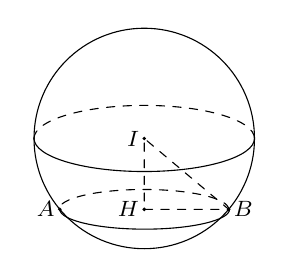
\begin{tikzpicture}[scale=0.7, font=\footnotesize,line join=round, line cap=round, >=stealth]
				\def\r{2}
				\def\a{1}
				\def\b{0.6}
				\pgfmathsetmacro\m{sin(40)}
				\pgfmathsetmacro\n{cos(40)}
				\path
				(0,0) coordinate (O)
				(\r*\n,-\r*\m) coordinate (M)
				(-\r*\n,-\r*\m) coordinate (N)
				(0,-\r*\m) coordinate (H)
				(0,\r) coordinate (A')
				(0,-\r) coordinate (A)
				;
				\draw	(O) circle (\r);
				\node at (O) [left] {$I$};
				\node at (M) [right] {$B$};
				\node at (N) [left] {$A$};
				\node at (H) [left] {$H$};
				%\node at (A') [above] {$A'$};
				%\node at (A) [below] {$A$};
				
				\fill (O) circle (1pt); 
				\fill (M) circle (1pt); 
				\fill (N) circle (1pt); 
				\fill (H) circle (1pt); 
				%\fill (A') circle (1pt); 
				%\fill (A) circle (1pt); 
				
				\draw	(180:\r) arc (180:360:{\r} and	{.3*\r});
				\draw[dashed]	(180:\r) arc (180:0:{\r} and	{.3*\r}) (H)--(M)--(O)--(H);
				
				\draw	(N) arc (180:360:{0.77*\r} and	{0.18*\r});
				\draw [dashed]	(M) arc (0:180:{0.77*\r} and	{0.18*\r});
		\end{tikzpicture}}
	}	
\end{bt}

\begin{bt}%[2H5H3-3]
% nguon: Archive/SP-4Phan-Dot3/Data/CTST_2-OTHK2-De06.tex #4563

	Lập phương trình mặt cầu $(S)$ biết mặt cầu $(S)$ có tâm $O(0;0;0)$ và tiếp xúc với mặt phẳng $(P)\colon 16x-15y-12z+75=0$.
	\loigiai{
		Phương trình mặt cầu $(S)$ có tâm $O(0;0;0)$ bán kính $R$ có dạng: $x^2+y^2+z^2=R^2$.\\
		Vì mặt cầu $(S)$ tiếp xúc với mặt phẳng $(P)$ nên
		\[R=\mathrm{d}\left(O;(P)\right)=\dfrac{|16\cdot0-15\cdot0-12\cdot0+75|}{\sqrt{16^2+(-15)^2+(-12)^2}}=3.
		\]
		Phương trình mặt cầu $(S)$ là $x^2+y^2+z^2=9$.
	}
\end{bt}

\begin{bt}%[2H5V3-3]
% nguon: Archive/SP-4Phan-Dot3/Data/CTST_2-OTHK2-De03.tex #4572

	Trong không gian $Oxyz$, cho các điểm: $A(2;3,0)$, $B(-2;1;0)$, $C(3;0;-2)$, $D(-2;3;0)$. Viết phương trình mặt cầu $(S)$ ngoại tiếp tứ diện $ABCD$.
	\loigiai{
		Phương trình mặt cầu $(S)\colon (x-a)^2+(y-b)^2+(z-c)^2=R^2$.\\
		Lần lượt thay tọa độ của $A, B, C, D$ vào $(S)$ ta giải hệ phương trình và tìm được $a=0$; $b=2$; $c=-3$; $R^2=14$.\\
		Vậy phương trình mặt cầu $(S)$ là $x^2+(y-2)^2+(z+3)^2=14$.
	} 
\end{bt}

\begin{bt}%[2H5H3-3]
% nguon: Archive/SP-4Phan-Dot3/Data/CTST_2-OTHK2-De02.tex #4584

    Trong không gian $Oxyz$, cho các điểm $A(-3; 0; 1), B(0;-2;-3), C(0; 0; 3), D(-3; 1; 1)$. Gọi $(S)$ là mặt cầu ngoại tiếp tứ diện $ABCD$. Viết phương trình mặt cầu $(S)$.
    \loigiai{
        Phương trình tổng quát của mặt cầu là $(S)\colon x^2+y^2+z^2-2ax-2by-2cz+d=0$.\\
        $(S)$ đi qua $A(-3; 0; 1), B(0;-2;-3), C(0; 0; 3), D(-3; 1; 1)$ nên ta có hệ phương trình \[\heva{&6a-2c+d=-10\\&4b+6c+d=-13\\&-6c+d=-9\\&6a-2b-2c+d=-11}\Leftrightarrow\heva{&a=\dfrac{1}{6}\\&b=\dfrac{1}{2}\\&c=-\dfrac{1}{2}\\&d=-12.}\]
        Suy ra phương trình mặt cầu $(S)$ là $$(S)\colon x^2+y^2+z^2-\dfrac{1}{3}x-y+z-12=0.$$
    }
\end{bt}

\begin{bt}%[2H5H3-3]
% nguon: Archive/SP-4Phan-Dot3/Data/CTST_2-OTHK2-De01.tex #4591

	Trong không gian $Oxyz$, cho hai điểm $A(4; 6; 8)$ và $B(2; 4; 4)$.	Gọi $(S)$ là mặt cầu đường kính $AB$. Viết phương trình mặt cầu $(S)$.
	\loigiai{
		Trung điểm của $AB$ là điểm $I(3;5;6)$. \\
		Tọa độ vectơ $\overrightarrow{AB}=(-2;-2;-4)$.\\
		Ta có $AB=\sqrt{4+4+16}=2\sqrt{6}$.\\
		Suy ra, mặt cầu $(S)$ có bán kính $R=\dfrac{AB}{2}=\sqrt{6}$.\\
		Với $I(3;5;6)$ là trung điểm của $AB$ và là tâm của mặt cầu $(S)$.\\
		Phương trình mặt cầu $(S)$ là $(x-3)^2+(y-5)^2+(z-6)^2=6$.
	}
\end{bt}
